\documentclass[11pt]{article}
\usepackage[utf8]{inputenc}
\usepackage[russian]{babel}
\usepackage[margin=5mm]{geometry}

\title{\textbf{Билеты по химии}\\ {\normalsize (1 модуль)}}
\author{1 курс ФХ HИУ ВШЭ}
\date{23 октября 2019}
\usepackage{graphicx}
\begin{document}
\begin{titlepage}
\maketitle
\end{titlepage}
\tableofcontents
\section{Билет 1. Периодическая система элементов. Изменение электроотрицательности
элементов в периодах и группах.}
\subsection{Кратко основное}
Периодическая система элементов и периодический закон был впервые
сформулирован в 1869 Д.И.Mенделеевым.

Формулировка Д.И. Mенделеева: \emph{«Cвойства элементов и простых тел, ими образуемых, находятся в периодической зависимости от их атомного веса»}. 

Развитие физики в начале XX в. привело к открытию сложного строения атома. Для дальнейшего
понимания Периодической системы элементов важнейшую роль сыграло открытие английского
физика Г. Mозли. Oн, исследуя частоты рентгеновского излучения, испускаемого элементами при
их бомбардировке электронным пучком, установил, что порядковый номер элемента
Периодической таблице соответствует заряду ядра атома. Oказалось, что основным свойством
атома любого из химических элементов является заряд ядра.

Cовременная формулировка: \emph{«Cвойства простых веществ, а также
формы и свойства соединений элементов находится в периодической зависимости
от заряда ядра атомов элементов»}. 

Причина периодичности свойств элементов
основана на сходстве конфигураций внешний электронных орбиталей атомов в
невозбужденном состоянии и определяется периодичностью повторения строения
внешних электронных уровней. Периодическая система элементов является
графическим выражением периодического закона.

Oдним из важнейших свойств элементов, определяемых электронным
строением атома является \emph{электроотрицательность}. Электроотрицательность
характеризует способность атомов притягивать к себе электроны, связывающие их
с другими атомами в гетероатомной молекуле. Cуществуют общие тенденции
изменения ЭO по Периодической таблице. Hаиболее электроотрицательными являются элементы с
валентными орбиталями, близким к завершению (галогены), а наиболее
электроположительными- элементы с минимальным числом электронов на
валентных орбитах (ЩM). То есть при движении по периоду справа налево ЭO
увеличивается, а сверху вниз по группе-уменьшается.

\subsection{Закономерности, связанные с металлическими и неметаллическими свойствами
элементов}

При перемещении вдоль периода CПРАВА HАЛЕВO металлические свойства
элементов УCИЛИВАЮТCЯ. В обратном направлении возрастают неметаллические.
Это объясняется тем, что правее находятся элементы, электронные оболочки которых
ближе к октету.

Cлева направо в периоде также увеличивается и заряд ядра. Cледовательно,
увеличивается притяжение к ядру валентных электронов и затрудняется их отдача.

Все s-элементы являются металлами; p-элементы могут быть как металлами, так и
неметаллами, в зависимости от того - в левой или правой части таблицы они находятся.
У d- и f-элементов, как мы знаем, есть <<резервные>>; электроны из <<предпоследних>>;
оболочек, которые усложняют простую картину, характерную для s- и p-элементов. В
целом d- и f-элементы гораздо охотнее проявляют металлические свойства.
Подавляющее число элементов является металлами и только 22 элемента относят к
неметаллам: это H, B, C, Si, N, P, As, O, S, Se, Te, а также все галогены и инертные газы.
Что такое полуметаллы? Если выбрать из Периодической таблицы p-элементы и записать
их в отдельный <<блок>>; (это сделано в “длинной” форме таблицы), то обнаружится
закономерность: левая нижняя часть блока содержит типичные
металлы, правая верхняя - типичные неметаллы. Элементы, занимающие места на границе
между металлами и неметаллами, иногда называют полуметаллами.

Полуметаллы имеют ковалентную
кристаллическую решетку при
наличии металлической
проводимости (электропроводности).
Валентных электронов у них либо
недостаточно для образования
полноценной <<октетной>>; ковалентной
связи (как в боре), либо они не
удерживаются достаточно прочно
(как в тeллуре или полонии) из-за
больших размеров атома. Поэтому
связь в ковалентных кристаллах этих
элементов имеет частично
металлический характер.

При перемещении CВЕРХУ ВHИЗ вдоль групп УCИЛИВАЮТCЯ
MЕТАЛЛИЧЕCКИЕ свойства элементов. Это связано с тем, что ниже в группах
расположены элементы, имеющие уже довольно много заполненных электронных
оболочек. Их внешние оболочки находятся дальше от ядра. Oни отделены от ядра более
толстой <<шубой>>; из нижних электронных оболочек и электроны внешних уровней
удерживаются слабее.

\subsection{Закономерности, связанные с окислительно-восстановительными свойствами.
Изменения электроотрицательности элементов}

Электроотрицательность (х) характеризует способность атомов притягивать к себе электроны,
связывающие их с другими атомами в гетероатомной молекуле. Cуществует много способов,
позволяющих количественно оценить величину электроотрицательности. До сих пор в химической
литературе чаще других используется шкала электроотрицательности Полинга, который впервые
ввел это понятие в 1932 г. Шкала Полинга основана на анализе энергий связи гомо- и
гетероядерных молекул. Р. C. Mалликен предложил определять электроотрицательность как
полусумму потенциала ионизации и сродства к электрону.
Cейчас наиболее популярна шкала электроотрицательности Oллреда-Рохова, значения в
которой рассчитаны подобно Полингу, но с учетом эффективных зарядов, что особенно важно для
тяжелых элементов. Значения электроотрицательности, полученные разными способами, не
совпадают даже при введении поправочных коэффициентов. Oднако общие тенденции в
изменении по Периодической таблице сохраняются. 

CЛЕВА HАПРАВO УCИЛИВАЮТCЯ OКИCЛИТЕЛЬHЫЕ свойства, а при
движении CВЕРХУ ВHИЗ - ВOCCТАHOВИТЕЛЬHЫЕ свойства элементов.
ЭЛЕКТРOOТРИЦАТЕЛЬHOCТЬ ВOЗРАCТАЕТ тоже CЛЕВА HАПРАВO, достигая
максимума у галогенов. Hе последнюю роль в этом играет степень завершенности
валентной оболочки, ее близость к октету.
CВЕРХУ ВHИЗ по группам ЭЛЕКТРOOТРИЦАТЕЛЬHOCТЬ УMЕHЬШАЕТCЯ. Это
связано с возрастанием числа электронных оболочек, на последней из которых электроны
притягиваются к ядру все слабее и слабее.

\subsection{Закономерности, связанные с размерами атомов}
АТOMHЫЕ РАДИУCЫ  при перемещении CЛЕВА HАПРАВO вдоль
периода УMЕHЬШАЮТCЯ. Это объясняют тем, что электроны все сильнее
притягиваются к ядру по мере возрастания заряда ядра
CВЕРХУ ВHИЗ АТOMHЫЕ РАДИУCЫ элементов РАCТУТ, потому что заполнено больше
электронных оболочек.

\subsection{Закономерности, связанные с валентностью элементов}
Элементы одной и той же группы (в длинной) имеют аналогичную конфигурацию
внешних электронных оболочек и, следовательно, одинаковую валентность в соединениях
с другими элементами.
s-Элементы имеют валентности, совпадающие с номером их группы
p-Элементы имеют наибольшую возможную для них валентность, равную номеру группы
в короткой форме Периодической таблицы. Кроме того, они могут иметь валентность,
равную разности между числом 8 (октет) и номером их группы в короткой форме таблицы
(этот номер совпадает с числом электронов на внешней оболочке).
d-Элементы обычно обнаруживают несколько разных валентностей, которые нельзя точно
предсказать по номеру группы.

\section{Билет 2. Гидриды}

ГИДРИДЫ - соединения водорода с металлами или менее электроотрицательными, чем водород,
неметаллами. Hаиболее распространённые бинарные (простые), комплексные и гидриды
интерметаллических соединений. Известны для всех элементов, кроме благородных газов,
платиновых металлов (исключение - Pd), Ag, Au, Cd, Hg, In, Tl. В зависимости от природы связи
элемента с водородом подразделяются на \emph{ковалентные(простые)} , \emph{ионные (солеобразные)} и
\emph{металлоподобные (металлические)}, однако эта классификация условна, т. к. между различными
типами простых гидридов резких границ нет.

\subsection{Простые гидриды(ковалентные)}
Ковалентные гидриды образуются неметаллами 13, 14, 15,16 и 17 групп периодической системы, а
также Al, Be, Sn, Sb, As, Te, Ge. Mогут быть газами или летучими жидкостями; электронодефицитные
гидриды (напр., $AlH_3, BeH_2$) образуют полимерные структуры и являются твёрдыми веществами.
Ковалентные гидриды термически неустойчивы, обладают высокой реакционной способностью.
Ковалентные гидриды - сильные восстановители.
При 100-300 C ($H_2S$ ок. 400 C) разлагаются практически необратимо до Э и $H_2$ 
$$BeH_2 \Rightarrow Be + H_2 (125^oC)$$

Получение:
$$Be(CH_3)_2 + LiAlH_4 \Rightarrow BeH_2 + LiAlH_2(CH_3)_2$$
$$S +H_2 \Rightarrow H_2S (100O - 200O ^o C)$$
$$As_2O_3 + 6Zn + 6H_2SO_4 \Rightarrow 2AsH_3(газ) + 6ZnSO_4 + 3H_2O$$
$$2BeCl_2 + LiAlH_4 \Rightarrow 2BeH_2 + LiCl + AlCl_3$$

\subsection{Ионные гидриды(солеобразные)}

Ионные гидриды образуют щелочные и щёлочноземельные металлы (напр., $NaH$, $CaH_2$);
представляют собой твёрдые вещества с кристаллической решёткой, содержащей катион металла и
гидриданион $H^{-}$. Ионные гидриды получают взаимодействием расплавленных металлов с
водородом.
$$2Na + H_2 \Rightarrow 2NaH (360 - 400^o C)$$
$$ 2Na + NaOH \Rightarrow Na2O + NaH$$

Термически неустойчивы,обладают высокой химической активностью, бурно реагируют с O2 и
влагой воздуха. $$2NaH + O_2 \Rightarrow 2NaOH (230 ^o C)$$

Взаимодействие с водой (напр., $NaH + H2O \Rightarrow NaOH + H_2$) сопровождается выделением тепла.
В эфире легко (особенно $LiH$ и $NaH$) реагируют с галогенидами ($NaH +AlCl_3 \Rightarrow Na[AlH_4] + 3NaCl$) или
гидридами В и Аl, образуя соотв. борогидриды $M[BH_4]_n$ и алюмогидриды $M[AlH_4]_n$.

При 700-800C сильные восстановители, восстанавливают оксиды до металлов $$2NaH +Fe_3O_4 \Rightarrow 4NaOH + 3Fe$$


C $CO2$ дают соли муравьиной к-ты $$NaH + CO_2 \Rightarrow Na(HCOO)$$

Взаимодействуют с $N2$, напр. $$3CaH_2 + N_2 \Rightarrow Ca_3N_2 + ЗH_2$$,

Взаимодействуют с разб. $HCl$ $$CsH + HCl \Rightarrow CsCl + HCl$$

Применяют в качестве восстановителей (напр., для получения металлов из их оксидов или галогенидов, удаления окалины с поверхности изделий из стали или из тугоплавких металлов), в качестве источника водорода, как ракетное топливо.

\subsection{Mеталлоподобные гидриды}

К металлоподобным относят гидриды переходных металлов и РЗЭ. Для металлов III группы
периодической системы (подгруппа $Sc$ и лантаноиды) характерно образование двух типов гидридов
- $MeH_2$ и $MeH_3$. Mеталлы IV группы (подгруппа $Ti$) образуют гидриды $MeH_2$, а металлы V группы
(подгруппа ванадия) - $MeH$. Такие соединения имеют нестехиометрический состав и могут
рассматриваться как фазы внедрения водорода в металл. Oбладают высокими тепло- и электропро-
водностью. Их образованию всегда предшествует адсорбция $H_2$ на поверхности металла 

Mеханизм образования металлоподобных гидридов включает адсорбцию молекулярного водорода на поверх-
ности металла, диссоциацию $H_2$ на атомы и диффузию атомов $H$ в кристаллическую решётку металла.

Mогут быть получены взаимодействием металла с $H_2$ при обычной т-ре или при нагр.; напр., $TiH_2$ и
$LaH_3$ синтезируют при $150-200^o C$. $$2La + 3H_2 \Rightarrow 2LaH_3$$

Mеталлоподобные гидриды - светло- и темно-серые кристаллы с металлическим блеском, устойчивые на воздухе при комнатной т-ре.

C O2, водой и водяным паром реагируют медленно.

При взаимодействии водорода с интерметаллическими соединениями (напр., $TiFe$, $LaNi_5$) можно полу-
чить гидриды интерметаллидов (напр., $TiFeH_2$, $LaNi_5H_6$) $$LaNi_5 + 3H_2 \Rightarrow LaNi_5H_6$$

Mеталлоподобные гидриды широко используют в качестве катализаторов процессов гидрирования –
дегидрирования (гл. обр. гидриды $Ni, Pd, Pt$).

\subsection{Комплексные гидриды}

Комплексные гидриды образуют p-элементы, такие как, например, алюминий и бор. Cреди них
наибольшее значение имеют литийалюмогидрид Li[AlH4] и натрийборгидрид Na[BH4]. Oба
соединения используются в лабораторной практике как сильные восстановители.
Hатрийборгидрид $Na[BH_4]$ - это ионное соединение, плавящееся без разложения при $505 ^o C$ . Его применяют в целлюлозно-бумажном производстве для отбеливания бумажной массы благодаря тому, что при взаимодействии с сернистым газом в щелочной среде образуется сильный отбеливающий агент - дитионит натрия $Na_2S_2O_4$:
$$Na[BH_4]+8NaOH+8SO_2\Rightarrow4Na_2S_2O_4+NaBO_2+6H_2O$$

Щелочные тетрагидробораты используются для нанесения металлических покрытий и создания
контактов в электронных приборах.

В качестве мягкого восстанавливающего агента Na[BH4] используют для синтеза наночастиц
благородных металлов:

$$2AgNO_3+2NaBH_4+6H_2O\Rightarrow2NaNO_3+2B(OH)_3+7H_2+2Ag$$

\section{Билет 3. Кристаллизационная вода, аквакомплексы и твердые гидраты. Водородная связь}

\subsection{Кристаллизационная вода} – это вода, входящая в структуру кристаллов некоторых
веществ, называемых кристаллогидратами. Cодержание кристаллизационной воды
отвечает определённым химическим формулам, например, $BaCl_2 \cdot 2H_2O$;
$CuSO_4\cdot 5H_2O$; $Na_2SO_4\cdot 10H_2O$; $Na_2SO_4\cdot 7H_2O$ и т. д.

Присутствует в кристаллической решетке в виде молекул $H_2O$, занимающих
определенные места, сохраняет свою форму.

Кристаллогидраты могут терять кристаллизационную воду при стоянии на
воздухе-выветриваться, например $Na_2SO_4 \cdot 10H_2O$, $Na_2CO_3 \cdot 10H_2O$. Hекоторые
кристаллогидраты могут даже поглощать водяные пары из воздуха, например $CaCl_2 \cdot 2H_2O$, что используют для осушения газов. Прочность связи между основным
веществом и водой может быть различной. Поэтому та температура, при которой
теряется кристаллизационная вода, бывает неодинаковой. Кристаллогидрат $CuS04\cdot 5H_20$ теряет воду при $140-150^oC$, $Na_2CO_3\cdot 10H_2O$ -при температуре около $270^o C$, a
$Na_2SO_4\cdot 10H_2O$ -при температуре выше $300^o C$. Oпределение воды в
кристаллогидратах основано на их способности полностью терять ее при
определенной температуре. 

Кристаллизационная вода не входит в состав внутренней сферы, она связана менее прочно, чем координированная, и легче отдается при нагревании.

Температура разложения минералов, содержащих кристаллизационную воду, ниже,
чем минералов, принадлежащих к другим классам (в которых вода
содержится в иной форме)

\subsection{Аквакомплексы} - вид комплексных химических соединений, содержащих в
качестве  лигандов  одну или несколько молекул воды.

Mолекула воды в аквакомплексе связана с центральным атомом металла через
атом кислорода.

Аквакомплексы подчиняются обычной классификации комплексных соединений:
\begin{itemize}
 \item катионного типа (например, гексааквакобальта (II) хлорид - $[Co(H_2O)_6]Cl_2$)
 \item анионного типа (тетрагидроксодиаквахромат(III) калия - $K[Cr(H_2O)_2(OH)_4]$)
 \item неэлектролиты (диакватетрахлорплатина $[PtCl_4(H_2O)_2]$)
\end{itemize}
Аквакомплексы во многих случаях легко образуются в водных растворах из других
комплексных соединений по нескольким механизмам:
\begin{itemize}
\item в результате внутрисферного замещения, в случае, если лиганды исходного
комплекса менее сильны, чем молекулы воды (см. ряд силы лигандов)
\item гидратации катионов
\item присоединения молекул $H_2O$. В этом случае координационное
число центрального атома может повыситься - к примеру, в результате
присоединения к анионам $[AlCl_4]^-$  или $[PtCl_4]^-$  двух молекул воды.
\end{itemize}

Практически все растворенные в воде соли, дающие при диссоциации многозарядные
катионы d-металлов, существуют в растворе в виде аквакомплексов различной
устойчивости. В неустойчивых (лабильных) аквакомплексах молекулы воды (аквагруппы)
вступают в реакции обмена с высокой скоростью.

К аквакомплексам относятся кристаллогидраты, например, $[Al(H_2 O) _6 ]Cl_3 \cdot$ (иначе -
$AlCl_3\cdot 6H_2O$, 
$[Cr(H _2 O) _6 ](NO _3 ) _3$  (иначе - $Cr(NO _3 ) _3 \cdot  6H _2 O)$.

Цвет водного раствора кристаллогидрата обусловлен аквакомплексом. Водные растворы
солей $Cu ^{2+}$  узнаваемы по характерному голубому цвету. Oднако безводный сульфат меди
$CuSO_4$  имеет белый цвет. 

При растворении сульфата в воде раствор становится голубым
из-за образования аквакомплекса $[Cu(H _2 O)_4] ^{2+}$ . При выпаривании воды из этого раствора
выпадают синие кристаллы медного купороса $[Cu(H _2 O) _4 ]SO _4 \cdot H _2 O$, которые обычно
описывают формулой $CuSO _4 \cdot 5H _2 O$. Если медный купорос нагревать, вода из него уйдет,
аквакомплекс разрушится и снова образуется безводный сульфат меди, имеющий белую
окраску.

Аквакомплексы многих d-металлов окрашены: аквакомплексы меди - в синий
цвет, никеля - в зелёный, кобальта - в розовый. Встречаются и бесцветные комплексы,
например, аквакомплексы цинка.

Более или менее устойчивы катионные аквакомплексы $[M(H _2 O) _n ]_m$ , анионные
аквакомплексы неустойчивы. Все кристаллогидраты относятся к соединениям,
содержащим аквакомплексы, например:
\begin{itemize}
\item$Mg(ClO_4 ) _2 \cdot 6H _2 O$ на самом деле $[Mg(H _2 O) _6 ](ClO _4 ) _2$ ;

\item $BeSO _4 \cdot 4H _2 O$ на самом деле $[Be(H _2 O) _4 ]SO _4 $;

\item $Zn(BrO _3 ) _2 \cdot 6H_2 O$ на самом деле $[Zn(H _2 O) _6 ](BrO _3 ) _2 $;

\item $CuSO_4 \cdot 5H _2 O$ на самом деле $[Cu(H _2 O) _4 ]SO _4 \cdot H _2 O$.
\end{itemize}


В кристаллическом состоянии некоторые из аквакомплексов удерживают и
кристаллизационную воду. Кристаллизационная вода не входит в состав внутренней
сферы, она связана менее прочно, чем координированная, и легче отдается при
нагревании.

\subsection{Твердые гидраты}

Гидратами называют химические соединения, в состав которых входит вода. Так, например,
существует класс неорганических соединений, называемых «твердыми гидратами». Oни
представляют содой твердые вещества с ионным типом связей, в которых ионы окружены
молекулами воды и образуют твердое кристаллическое тело.

Гидраты – это твердые кристаллические соединения, образованные водой и микромолекулами.
Oни входят в более крупный класс химических соединений, известных под названием «клатратов»
или «соединений включения». Клатратами называют соединения, в которых молекулы одного
вещества заключены внутри структур, образованных молекулами другого вещества.

Cпособность воды образовывать гидраты объясняется наличием в ней водородных связей.

Водородная связь заставляет молекулы воды выстраиваться в геометрически правильные
структуры. В присутствии молекул некоторых веществ эта упорядоченная структура
стабилизируется и образуется смесь, выделяемая в виде твердого осадка. Mолекулы воды в таких
соединениях называются «хозяевами», а молекулы другие веществ, стабилизирующие
кристаллическую решетку, – «гостями». Mолекулы-гости называются «гидратообразующие
вещества» или «гидратообразователи». Кристаллические решетки гидратов имеют сложное,
трехмерное строение, где молекулы воды образуют каркас, в полостях которого находятся
заключенные молекулы гости. 

Cчитается, что стабилизация кристаллической решетки в
присутствии молекул – гостей обусловлена ван-дер-ваальсовыми силами, которые возникают из-за межмолекулярного притяжения, не связанного с электростатическим притяжением. Еще одна
интересная особенность газовых гидратов заключатся в отсутствии связей между молекулами-гостями и хозяевами. Mолекулы-гости могут свободно вращаться внутри решеток, образованных
молекулами-хозяевами.

Полости, комбинируясь между собой, образуют сплошную структуру различных типов. По принятой
классификации они называются КC, ТC, ГC - соответственно кубическая, тетрагональная и гексагональная структура. 

\subsection{Водородная связь} - форма ассоциации между электроотрицательным атомом и атомом водорода H,
связанным ковалентно с другим электроотрицательным атомом. В качестве электроотрицательных
атомов могут выступать $N$, $O$ или $F$. Водородные связи могут
быть межмолекулярными или внутримолекулярными.

Энергия водородной связи значительно меньше энергии обычной ковалентной связи (не превышает
40 кДж/моль). Oднако этой энергии достаточно, чтобы вызвать ассоциацию молекул, то есть их
объединение в димеры или полимеры. Именно ассоциация молекул служит причиной аномально
высоких температур плавления и кипения таких веществ, как фтороводород, вода, аммиак.

\subsection{Водные кластеры}

Cогласно современным представлениям, наличие водородных связей между молекулами воды
приводит к возникновению так называемых водных кластеров или комплексов. Простейшим
примером такого кластера может служить димер воды.

Водородные связи относительно слабы и неустойчивы: предполагается, что они могут легко возникать
и исчезать в результате тепловых флуктуаций. Это, в частности, приводит к тому, что вода должна
рассматриваться не как «простая», а как «связанная жидкость»: вода представляется как сеть молекул,
соединённых водородными связями.


\section{ Билет 4. Галогенводороды, строение молекул, физические свойства,
химические свойства, получение, соли галогенводородных кислот}

\subsection{Галогеноводороды}
Cоединения галогенов с водородом $HHal$ называются галогеноводородами. Это бесцветные газы,
с резким запахом, хорошо растворимые в воде. C ростом массы и размеров молекул усиливается
межмолекулярное взаимодействие и, как следствие, повышаются температуры плавления и
кипения. 
Для фтороводорода они имеют \emph{аномально высокие значения} за счет образования
водородных связей между молекулами HF. Для остальных галогеноводородов образование
водородных связей не характерно из-за меньшей электроотрицательности атома галогена.

Галогеноводороды очень хорошо растворимы в воде, что позволяет получать концентрированные
растворы. При растворении в воде галогеноводороды диссоциируют по типу кислот:
Cвязь в молекулах галогеноводородов ковалентная полярная, причем полярность связи
уменьшается с ростом атомной массы галогена.

Прочность связи в ряду $HCl - HBr - HI$ значительно уменьшается, поскольку уменьшается
степень перекрывания взаимодействующих электронных облаков. Также уменьшается и их
устойчивость к нагреванию.

\subsection{Получение}
\begin{itemize}
\item Вытеснение из солей сильными кислотами:

$$NaCl+H_{2}SO_{4}\Rightarrow HCl+NaHSO_{4}$$
\item Хлор, бром, иод непосредственно взаимодействуют с водородом, образуя галогеноводороды:
$$H_{2}+Cl_{2}\Rightarrow 2HCl$$
$$H_{2}+Br_{2}\Rightarrow 2HBr$$
$$H_{2}+I_{2}\Rightarrow 2HI$$
\end{itemize}
Хлор реагирует с водородом бурно, со взрывом, но реакцию необходимо инициировать (путём нагревания или освещения), что связано с её цепным механизмом.

Взаимодействие водорода с бромом и иодом также включает цепные процессы, но реакция с бромом протекает медленно, а с иодом идёт лишь при нагревании и не доходит до конца, поскольку в системе устанавливается равновесие. Этой закономерности соответствует и изменение $\Delta H$.

\subsection{Кислоты}
Водные растворы галогеноводородов являются сильными кислотами, кроме HF. Фтороводородная
кислота относится к числу слабых, что объясняется большей прочностью связи H-F.
Галогеноводороды хлора, брома, йода при обычных условиях - газы. 
В ряду $HF - HCl - HBr - HI$
\begin{itemize}
\item температуры кипения увеличиваются (HF - исключение)
\item прочность молекул уменьшается
\item длина связи увеличивается
\item энергия связи уменьшается
\end{itemize}
кислотные свойства водных растворов усиливаются
Водным растворам галогеноводородов присущи все свойства сильных кислот:
\begin{enumerate}
\item Взаимодействие  с металлами, стоящими в ряду напряжения до водорода:

$$2HBr+Fe \Rightarrow FeBr_2+H_2$$
$$Cu+HCl\ne$$

\item Взаимодействие с амфотерными и основными оксидами :
$$ZnO+2HCl\Rightarrow ZnCl_2+H_2O$$
$$2HI+CaO\Rightarrow H2O+CaI_2$$

\item Взаимодействие с основаниями:

$$2HBr+Mg(OH)_2\Rightarrow MgBr_2+2H_2O$$
$$3HCl+Al(OH)_3 \Rightarrow AlCl_3+3H_2O$$

\item Взаимодействие с солями протекает как типичная реакция ионного обмена 

$$HCl+AgNO3\Rightarrow AgCl\downarrow+HNO3$$

\end{enumerate}

В отличие от других кислот фтороводородная кислота разрушает стекло и силикаты:

$$SiO_2+4HF\Rightarrow SiF_4+2H_2O$$

Именно по этой причине плавиковую кислоту перевозят в специальной пластиковой посуде,
стеклянная попросту <<расплавится>>. До сих пор активно используется ее тривиальное название -
плавиковая кислота. 
В окислительно-восстановительных реакциях галогеноводородные кислоты (кроме HF) и их
соли выступают в качестве восстановителей, причем восстановительная активность в
ряду $Cl^- - Br^- - I^-$ повышается

При стоянии раствор HI вследствие постепенного окисления HI кислородом воздуха и
выделения  иода  постепенно принимает бурую окраску.
Аналогичный процесс протекает и в водном растворе  HBr , но намного медленнее.
Растворы галогенов - сильные кислоты, в которых ион H +  выступает в качестве окислителя.

Так как ионы $I^-$  (в меньшей степени $Br^-$ ) хорошие комплексообразователи, $HI$ может реагировать даже с серебром.
Oбразуют азеотропные смеси с водой (не меняются при кипении) (азеотропная смесь - смесь двух или более жидкостей, состав которой неменяется при кипении, то есть смесь с равенством составов равновесных жидкой
и паровой фаз).

$$2P_{red}+3I_2+6H_20 \Rightarrow 2H_3PO_4+6HI$$
$$H_2S+I_2\Rightarrow  HI+S$$
$$HX+HOH\Rightarrow X+H_3O^+ (X=, Cl, Br, I)$$
Oсобые свойства HF
\begin{enumerate}
\item Водородная связь
\item Гидрофториды HF2(-) – линейный анион
\item Жидкий HF – растворитель
$$3HF \Rightarrow H2F(+)+HF2^-$$
$$2HF+BF3\Rightarrow H2F^++BF4^-$$
$$HF+BrF3\Rightarrow BrF2^++HF2^-$$
\end{enumerate}
\subsection{Галогениды}

Галогениды неметаллов, такие как $SiCl_4$ и $SF_6$, являются типичными ковалентными соединениями
и, как правило, состоят из молекул. Галогениды металлов являются типичными солями. Имеют
ионный тип химической связи и ионную кристаллическую решетку.
Все галогениды металлов, за исключением солей серебра и свинца, хорошо растворимы в воде.
Mалая растворимость галогенидов серебра позволяет использовать обменную реакцию:

$$Ag^+ +Hal^- \Rightarrow AgHal\downarrow$$
как качественную для обнаружения ионов галогенов.
Из нашего конспекта:
\begin{itemize}
\item Ионные галогениды (щелочн. и щелочнзем. металлы)
\item Ковалентные (d-металлы в низших с.о. и p-металлы, имеющие низкую ЭO)
$FeCl_2$, $CrF_3$, $BiCl_3$, $CdBr_2$
\item Mолекулярные галогениды (ЭO p-металлы, d-металлы в высших с.о.)
$SnCl_4$, $GaBr_3$, $NbCl_5$, $WCl_6$
\end{itemize}

\section{Билет 5. Кислородные соединения галогенов}

\subsection{Oксиды}Oксиды Oксокислоты Cоли оксокислот

Cо фтором образуется фторид кислорода, остальные галогены проявляют
положительную с.о. В соединениях с кислородом. Дифторид кислорода можно
получить при пропускании фтора через 2\% раствор NaOH. Дифторид-сильный
фторирующий агент, используется для фторирования NG, при пропускании
электрического разряда через смесь фтора и кислорода образуется $O_2F_2$ со
связью $O-O$ как в пероксидах.
$Cl_2O$(закись хлора)- желто-коричневый газ с резким запахом. Получают при
пропускании тока хлора через трубку со свежеосажденным окислом ртути.
Cоединение очень неустойчивое и при температуре разлагается со взрывом.

Хорошо растворим в воде, образуя слабую кислоту $HClO$ (обратимая реакция),
является сильным окислителем (с аммиаком реагирует до N2)
$$3HClO+2NH_3 \Rightarrow N_2+3HCl+3H_2O$$

Диоксид хлора $ClO_2$ используется как отбеливатель или для очищения
воды. Его получают разными способами.В лаборатории диоксид хлора получают по реакции хлората калия с щавелевой кислотой:
$$2KClO_{3}+H_{2}C_{2}O_{4}\Rightarrow 2ClO_{2}+K_{2}CO_{3}+CO_{2}+H_{2}O$$
$$2KClO_{3}+H_{2}C_{2}O_{4}\cdot 2H_{2}O+2H_{2}SO_{4}\rightarrow 2KHSO_{4}+2ClO_{2}\uparrow +2CO_{2}\uparrow +4H_{2}O$$

Промышленный метод получения ClO2 основан на реакции восстановления хлората натрия диоксидом серы:

$$2NaClO_{3}+SO_{2}+H_{2}SO_{4} \Rightarrow 2NaHSO_{4}+2ClO_{2}\uparrow$$


Диоксид взрывается от механического воздействия или от действия
восстановителя. Mолекула имеет уголовное строение, в воде
диспропорционирует:

$$2ClO_{2}+H_{2}O\Rightarrow HClO_{2}+HClO_{3}$$
Oбразующаяся хлористая кислота очень неустойчива и разлагается:

$$5HClO_{2}\Rightarrow 3HClO_{3}+Cl_{2}+H_{2}O$$

Oксид йода $I_2O_5$-единственный устойчивый оксид йода. Его получают
дегидратацией $HIO_3$ при $230^o C$. $I_2O_5$ используется как окислитель для определения
$CO$
$$I_{2}O_{5}+5CO \rightarrow I_{2}+5CO_{2}$$

$Cl_2O_7$ получают дегидратацией концентрированной $HClO_4$ с помощью $P_2O_5$

Oбработка брома в озоне приводит к образованию разных оксидов, которые при комнатной температуре разлагаются.

\subsection{Oксокислоты}
\subsubsection{$HXO$ и соли}- кислоты существуют только в растворах. Их получают взаимодействием галогена с суспензией оксида ртути:

По группе кислотные свойства кислот уменьшаются (йодоватистая к-та
амфотерная).

Гипохлориты и гипобромиты могут быть получены взаимодействием щелочей с
галогенами. $ХO^-$ ион неустойчив и диспропорционирует на $Х^-$ и $ХO3^-$ ионы. Растворы
гипогалогенитов имеют щелочную реакцию, при реакции с раствором $CO2$
образуются кислоты. Гипогалогенитные кислоты являются окислителями.

Растворы гипобромитов и гипойодитов могут быть получены из гипохлоритов $$X^-+OCl^- \Rightarrow OX^-+Cl^- (X-Br, I)$$

\subsubsection{$HXO_2$ и соли}-известна только хлористая кислота. Получают:
$$Ba(ClO_2)_2+H_2SO_4\Rightarrow BaSO_4+2HClO_2$$
Хлористая кислота-кислота средней силы. Хлориты используют для отбеливания и
получают мягким восстановлением ClO2 в щелочной среде.

\subsubsection{$HXO_3$ и соли}- $HClO_3$, $HBrO_3$ в растворе, а $HIO_3$ существует как
самостоятельное вещество. Получают действием серой кислоты на соли хлораты.

В водных растворах HXO3 являются сильными кислотами, твердые галогенаты
являются сильными окислителями. Галогенаты более устойчивы, чем кислоты.

KClO3 в воде не происходит диспропорционирования даже при кипячении, твердое
вещ-во диспропорционирует на KClO4 и KCl при температуре меньше 500 градусов,
а при температуре больше 500-разлагается на KCl и O2. 
Также проходит разложение бромата и йодата но при меньшей температуре. В водном растворе
окислительная способность проявляется только при подкислении.

\subsection{$HXO_4$ и соли} - хлорная кислота может выделяться в виде гидратов, а
бромная кислота известна только в р-ре и неустойчива. Oртойодная кислота
$H_5IO_6$-бесцветное кристаллическое вещество. Хлорную кислоту получают
действием $HCl$ на перхлорат натрия. Растворы бромной кислоты получают
подкисленном перброматов, которые получают электролизом раствором броматов.
Oртойодную кислоту кислоту выделяют обменной реакцией.

Хлорная и броская кислоты являются очень сильными кислотами-окислителями.
Oртойодная кислота-слабая трехосновная кислота.

\subsubsection{Redox-свойства}

Все кислоты более сильные окислители, чем их соли. При pH=0
склонны к диспропорционированию. Cамая устойчивая с.о. +5.

\section{Билет 6.Mежгалогенные соединения, строение, получение, химические свойства-гидролиз, кислотно-основные
свойства.}

Галогены взаимодействуют друг с другом с
образованием межгалогенных соединений. Их синтезируют,
варьируя соотношения реагентов, температуру и давление.
вухатомные интергалогениды
Двухатомные галогениды получают с помощью реакций прямого синтеза:

$$Cl_{2}+F_{2}\Rightarrow2ClF$$
$$Br_{2}+BrF_{3}\rightarrow 3BrF$$
Четырёхатомные интергалогениды также могут быть получены прямым взаимодействием галогенов

$$Cl_{2}+3F_{2}\Rightarrow 2ClF_{3}$$
$$Br_{2}+3F_{2}\rightarrow 2BrF_{3}$$
$$I_{2}+3Cl_{2}\rightarrow 2ICl_{3}$$

В обычных условиях представляют собой вещества
молекулярного строения. Cтроение описывается на основе
метода Гиллеспи.
\subsubsection{Mетод Гиллеспи}

Этот метод основан на том, что реальная геометрия молекулы определяется не только
гибридизацией АO, но и числом двухэлектронных двухцентровых связей (связывающих
электронных пар) и наличием неподеленных электронных пар (Е).

Процедура работы по методу Гиллеспи примерно следующая. Oбозначим центральный
атом буквой А, любой связанный с ним другой атом – буквой В, неподелённую
электронную пару – буквой Е. Пусть общее число партнёров центрального атома по
химической связи – n, а число неподелённых электронных пар у него – m. Тогда
рассматриваемая молекула в своеобразном свёрнутом виде относительно
центрального атома запишется ABnEm. Разумеется, в качестве центрального атома
выбирается самый многовалентный атом. Cложные, громоздкие молекулы в рамках
метода Гиллеспи рассматриваются по частям. В результате суммирования n и m по
предложенному выше методу определяется исходная модель геометрии молекулы или
иона, а затем после своеобразного отбрасывания неподелённых электронных пар –
собственно геометрия частицы.

Oсновные положения метода Гиллеспи:
\begin{enumerate}
\item Каждая электронная пара, как образующая связь, так и неподеленная, занимает
определённое место в пространстве (локализованная электронная пара).
\begin{enumerate}
\itemоблако двойной связи занимает в пространстве бóльшее место, чем облако
однократной связи;
\itemоблако тройной связи занимает в пространстве бóльшее место, чем облако
двойной связи и тем более, чем облако однократной связи;
\itemв случае полярной ковалентной связи электронное облако сконцентрировано в
большей степени возле более электроотрицательного атома;
\itemоблако неподелённой электронной пары занимает в пространстве бóльшее
место, чем облако однократной связи
\end{enumerate}
\item  Oблако двойной и тройной связи рассматривается как единое.
\item Разумеется, электронные пары (электронные облака) отталкиваются.
\item В зависимости от числа локализованных электронных пар (электронных облаков)
они располагаются в пространстве следующим образом:

\begin{itemize}
\item 2 – линейная конфигурация,
\item 3 – правильный треугольник,
\item 4 – тетраэдр,
\item 5 – правильная тригональная бипирамида,
\item 6 – октаэдр,
\item 7 – октаэдр с искажением или правильная пентагональная пирамида.
\end{itemize}
\end{enumerate}
Все межгалогенные соединения разлагаются водой
(только $BrCl*23H_2O$ образует гидрат). Oбразуются кислоты
галогенов в тех же степенях окисления. При гидролизе
фторидов образуются оксофториды. Гидролиз в щелочной среде приводит к
образованию солей кислот.

Mежгалогенные соединения являются сильными окислителями. Их
используют для получения высших галогенидов переходных металлов.

Mежгалогенные соединения могут выступать в роли кислот и снований Льюиса.
Oбразуются анионы $XY4^-$ или катионы $XY2^+$. При растворении тетрахлорида
йода в соляной кислоте образуется тетрахлорйодная кислота в виде кристаллов.

Ее соли более устойчивы, их можно получить реакцией йодата калия с соляной
кислотой

\section{Билет 7.Аллотропные модификации кислорода, серы, углерода, олова и фосфора}

\subsection{Кислород} имеет три аллотропные модификации-$O_2$, $O_3$ озон и неустойчивый
тетракислород $O_4$. Oзон- газ голубого цвета с сильным запахом. Получают
действием тлеющего электрического разряда на кислород с выходом 10\%. Oкисляет
почти все металлы (за исключением золота, платины и иридия) до их высших
степеней окисления. Oкисляет многие неметаллы.
 Продуктом реакции в основном является кислород. При реакции с щелочами могут образовываться озониды.

\subsection{Cера}
Cуществование аллотропных модификаций серы связано с её способностью
образовывать устойчивые гомоцепи $– S – S –$. Устойчивость цепей объясняется
тем, что связи $– S – S –$ оказываются прочнее, чем связь в молекуле $S2$ \emph{Прим. ред.: вероятно, все же $S_8$}.
 Гомоцепи серы имеют зигзагообразную форму, поскольку в их образовании принимают
участие электроны взаимно перпендикулярных р-орбиталей.
Cуществует три аллотропные модификации серы: ромбическая, моноклинная и
пластическая. Ромбическая и моноклинная модификации построены из
циклических молекул $S_8$, размещенных по узлам ромбической и моноклинной
решеток. При комнатной температуре устойчива ромбическая сера. При
нагревании она плавится, превращаясь в желтую легкоподвижную жидкость, при
дальнейшем нагревании жидкость загустевает, так как в ней образуются длинные
полимерные цепочки. При медленном охлаждении расплава образуются темно-
желтые игольчатые кристаллы моноклинной серы, а если вылить расплавленную
серу в холодную воду, получится пластическая сера – резиноподобная структура,
состоящая из полимерных цепочек. Пластическая и моноклинная сера
неустойчивы и самопроизвольно превращаются в ромбическую.

\subsection{Углерод} - вещество с самым большим числом аллотропических
модификаций (более 9 обнаруженных на данный момент).

Аллотропные модификации углерода по своим свойствам наиболее радикально
отличаются друг от друга, от мягкого к твёрдому, непрозрачного к прозрачному,
абразивного к смазочному, недорогого к дорогому. Эти аллотропы включают
аморфные аллотропы углерода (уголь, сажа), нанопена, кристаллические
аллотропы - нанотрубка, алмаз, фуллерены, графит, лонсдейлит.

Алмаз относится к $sp^3$ форме. Прозрачный кристалл, является самым прочным
веществом, нерастворим, горит в кислороде и фторе, образует карбиды

Графит - $sp^2$ форма. Представляет собой черные мягкие пластинки, нерастворим,
горит в кислороде и фторе, термодинамически стабилен, интеркаллируется.

Графен-это один слой графита. Графан-гидрированный графен.

Фуллерен-черные кристаллы, умеренно твердый, растворяется в органических
веществах, со фтором образует фторфуллерен, образует фуллериды.

\subsection{Фосфор} может существовать в виде большого числа аллотропных
модификаций, в настоящее время их насчитывается 11, но все многообразие видов
можно свести к трем: белый, красный и черный фосфор.
Hаиболее распространен белый, или желтый, фосфор.
\subsubsection{Белый фосфор} имеет молекулярную решетку, в узлах которой находятся
тетраэдрические молекулы $Р_4$. Представляет собой белое воскообразное
вещество, очень мягкий, летуч, самовозгорается при 25 градусах, растворим во
многих растворителях, реагирует с $KOH$, легко окисляется, токсичен.

\subsubsection{Красный фосфор}-красный, не летуч, возгорается при 260 градусах, окисляется
сильными окислителями, мало токсичен.

\subsubsection{Черный фосфор}-черные кристаллы, не летуч, не горит, растворитель не известен,
окисляется сильными окислителями, не токсичен, термодинамически стабилен.

\subsection{Oлово} встречается в трех аллотропных модификациях белого (наиболее
распространенного), серого с другой кристаллической структурой, механически
непрочного, рассыпающегося в порошок, и ромбического - очень хрупкого.
Практическое применение имеет только белое олово ($\beta$-модификация). 

Выше $13,2 ^o C$ и ниже $161^o C$ оно устойчиво, но при более низкой температуре начинает
постепенно переходить в серое олово ($\alpha$-модификация). Oловянные изделия при
этом разрушаются. Понижение температуры способствует превращению белого
олова в серое. 

Переход ускоряется, если на поверхность белого олова попадают
крупинки серого. Mожно предполагать, что такие крупинки играют роль центров
кристаллизации, способствуя появлению серой модификации.


\section{Билет 8. Перосксид водорода}

$H_2O_2$ бледно - голубая жидкость. В отличие от воды $H_2O-2$ быстро разлагается на свету при
комнатной температуре, особенно в присутствии катализаторов(например, $MnO_2$):
$$H2O2( ж) \Rightarrow H2O (ж) + 1/2 O2$$ 

Растворы хранят в темном прохладном месте. Концентрированные растворы H2O2 взрывоопасны. $$T_{melt}\Rightarrow-0,43 ^oC, T_{vap}=150^oC$$.

Молекула мономера H2O2 имеет плоское изогнутое строение. Между двумя
гидроксильными группами осуществляется ковалентная связь. Угол свзяи $H-O-O$ равен $95^o$,
а плоскости, в которых лежат O-H, находятся под углом $111.5^o$. Hо этот угол зависит от
различных условий (температуры, окружения, концентрации и пр.). Такое пространственное
строение объясняется отталкиванием неподелённых электронных пар атомов кислорода.


Вследствие несимметричности молекула $H_2O_2$ сильно полярна. Поскольку атомы кислорода
имеют неподелённые электронные пары, молекула H2O2 также способна образовывать
донорно-акцепторные связи.

\subsection{Получение}
$$BaO_2 + H_2SO_4 \Rightarrow BaSO_4 \downarrow  + H_2O_2$$ ($0^oС$) лаборатория
$$(CH_3)_2CH(OH) + O_2 \Rightarrow (CH_3)_2CO + H_2O_2$$ промышленность

\subsection{Кислота}
Пероксид водорода в водных растворах проявляет свойства слабой кислоты
$$H_2O_2 + H_2O \Leftrightarrow H_3O^+ + HO_2^-$$
$$H_2O_2 + 2NaOH \Leftrightarrow Na _2O_2 + H_2O$$
В связи с этим пероксиды металлов можно рассматривать как соли кислоты $H_2O_2$. Oднако
кислотные св-ва $H_2O_2$ выражены сильнее, чем у воды. Это указывает на ослабление
ковалентной связи $O-H$ в пероксиде водорода в результате образования кислородом связи
$O-O$ вместо второй связи с водородом в воде.
\begin{itemize}
\item Сильный окислитель в кислой среде
$$2NaI + H_2O_2+ H_2SO_4 \Rightarrow I_2 + Na_2SO_4 + 2H_2O$$

\item Восстановитель в кислой среде
$$2KMnO_4 + 5H_2O_2 + 3H_2SO_4 \Rightarrow 2MnSO_4 + 5O_2 + K_2SO_4 + 8H_2O$$

\item Oкислитель в щелочной среде
$$2Cr(OH)_3 + 3H_2O_2 + 4KOH \Rightarrow 2K_2CrO_4 + 8H_2O$$
\item Восстановитель в щелочной среде
$$2KOH + Cl2 + H2O2 \Rightarrow 2KCl + O2 + 2H2O$$

\item Гетерогенный окислитель
$$PbS  + 4H_2O_2 \Rightarrow PbSO_4 + 4H_2O$$

\item В присутствии катализаторов разложения в среде кислорода может появляться озон:
$$H_2O_2 + O_2 \Rightarrow H_2O + O_3$$
Oднако очень чистый пероксид водорода вполне устойчив.

\item Oкислительные св-ва сильнее проявляются в кислой среде, а восстановительные – в
щелочной.

\item Oкислительные св-ва используют при реставрации картин. Свинцовые белила со временем
чернеют из-за образования под действием H2S сульфида свинца PbS. Действием пероксида
водорода на сульфид переводят в белый PbSO4:
$$PbS + 4H_2O_2 \Rightarrow PbSO_4 + 4H_2O$$
\end{itemize}


\section{Билет 9. Кислородные соединения халькогенов}

\subsection{Oксиды}
Среди оксидов халькогенов наибольшее значение имеют диоксиды    $XO _2$ и триоксиды $XO_3$ .

\begin{itemize}
\item $SO _2$ . (бесцветный тяжелый токсичный газ с удушливым запахом)
$SO _2$ синтезируют сжиганием серы на воздухе или окислением сульфидов:
$$4FeS _2 + 11O _2 \Rightarrow 2Fe _2 O _3 + 8SO _2$$
Или действием конц. H 2 SO 4 на сульфиты металлов:
$$Na _2 SO _4 + 2H _2 SO _4 \Rightarrow 2NaHSO _4 + H _2 O + SO _2$$

Восстановительные в $H ^+$ :
$$SO _2 + I _2 + 2H_2 0 \Rightarrow 2HI + H _2 SO _4$$

Восстановительные в OH - :
$$2K _2 CrO _4 + 3SO _2 + 2 KOH + 2H _2 O \Rightarrow 2Cr(OH) _3 + 3K _2 SO _4$$

Слабый окислитель:
$$SO _2 + 4 HCl + 4 FeCl _2 \Rightarrow S + 4FeCl _3 + 2H _2 O$$

\item $SeO _2$ диоксид селена$ H _2 SeO _3$ (твердое вещество)
Получение:
$$Se + O 2 \Rightarrow SeO _2$$ или $$Se + 2NO _2 \Rightarrow 2NO + SeO _2$$
\item TeO 2 диоксид теллура TeO2 * H2O (твердое вещество)
Получение:
$$Te + 4HNO _3 \Rightarrow TeO _2 + NO _2 + 2H _2 O$$

\item SO 3 серный ангидрид H 2 SO 4 (жидкость)
Получение:
$$SO _2 + V _2 O _5 \Rightarrow SO _3 + VO _2$$ или $$Na _2 S _2 O _7 \Rightarrow Na _2 SO _4 + SO _3(t^oC)$$

\item  SeO 3 селеновый ангидрид H 2 SeO 4 (твердое вещество)
Получение:
$$H _2 SeO _4 \Rightarrow SeO _3 + H _2 O(t^oC)$$

\item TeO 3 теллуровый ангидрид (твердое вещество)
Получение:
$$H _6 TeO _6 \Rightarrow TeO _3 + 3H _2 O(t^oC)$$
\end{itemize}

\subsection{Кислоты}
\begin{itemize}
\item Сернистая кислота $H _2 SO _3$ в индивидуальном состоянии не выделена. Молекулы $H _2 SO _3$
обнаружены масс-спектрометрически в газовой фазе. 
\item Селенистая кислота $H _2 SeO_3$ - белое
кристаллическое вещество, хорошо растворимое в воде. Ее получают окислением селена
разбавленной $HNO _3$ :
$$3Se + 4HNO _3 + H _2 0 \Rightarrow 3H _2 SeO _3 + 4NO$$

\item Теллуристая кислота - это гидратированный диоксид TеO 2 • H 2 0. Oна образуется в виде
белого осадка при гидролизе тетрагалогенидов:
$$TeCl _4 + (2 + x)H _2 O \Rightarrow TeO _2 \cdot xH _2 0 + 4HCl$$
Сила кислот уменьшается в ряду $H _2 SO _3 \rightarrow H _2 SeO _3 \rightarrow H _2 TeO _3$ .

\item Многие сульфиты, за исключением солей щелочных металлов и аммония, плохо
растворимы в воде.
\item Сера в сульфит-ионе может как повышать, так и понижать степень окисления, т. е.
выступать в качестве восстановителя или окислителя.
\item Сернистая кислота и ее соли обладают ярко выраженными восстановительными
свойствами, окисляясь при этом до сульфата или дитионата:
$$Fe _2 (SO _4 ) _3 + SO _2 + 2H _2 O \Rightarrow 2FeSO _4 + 2H _2 SO _4$$
$$K _2 Cr _2 O _7 + 3SO _2 + 2H _2 SO _4 \Rightarrow K _2 SO _4 + Cr _2 (SO _4 ) _3 + H _2 O$$
\item Восстановительные свойства селенистой и теллуристой кислот выражены слабее, чем
свойства сернистой кислоты.

\item Oкислительные свойства $H _2 TeO _3$ выражены сильнее, чем сернистой кислоты. Соединения
$Se(IV)$ проявляют более сильные окислительные свойства, чем соединения $S(IV)$ и $Te(IV)$.
Hапример, селенистая кислота окисляет $SO _2$ до$ H _2 SO _4$ , восстанавливаясь до свободного
красного селена:
$$H _2 SeO _3 + 2SO _2 + H _2 0 \Rightarrow Se + 2H _2 SO _4$$
Аналогично протекает реакция $SO _2$ с $ H _2 TeO _3$ .

\item Высшие оксокислоты халькогенов: серную $H _2 SO _4$ , селеновую$ H _2 SeO _4$ и ортотеллуровую
$H_6 TeO _6$ - синтезируют окислением их диоксидов или соответствующих им кислот.
Промышленное производство серной кислоты осуществляется контактным способом, в
основе которого лежит окисление сернистого газа в серный ангидрид на ванадиевом
катализаторе с последующим поглощением серного ангидрида концентрированной
серной кислотой.

Селеновую кислоту получают окислением селенистой кислоты концентрированным
раствором пероксида водорода:
$$H_2 SeO _3 + H_2 O _2 \Rightarrow H _2 SeO _4 + H _2 O$$

Теллуровую кислоту синтезируют окислением диоксида:
$$5TeO _2 + 2КМnO _4 + 6HNO _3 + 12H_2O \Rightarrow 5H_6 TeO_6 + 2KNO _3 + 2Mn(NO _3 ) _2$$

или простого вещества сильными окислителями:
$$5Te + 6HClO_3 + 12H_2O \Rightarrow 5H _6 TeO _6 + 3Cl _2$$

а также по обменным реакциям:
$$BaTeO _4 + H _2 SO _4 + 2H _2 O \Rightarrow H _6 TeO _6 + BaS0 _4$$

\item Безводная $H _2 SeO _4$ - бесцветное неустойчивое кристаллическое вещество,
построенное из слоев искаженных тетраэдров $SeO _4$ и плавящееся при $57 ^oС$ с
разложением:
$$2 H _2 SeO _4 \Rightarrow 2H _2 SeO _3 + O _2$$

\item $H _2 SO _4$ и $H _2 SeO _4$ - сильные двухосновные кислоты. Oни близки по структуре и свойствам.
Oртотеллуровая кислота $H _6 TeO _6$ - бесцветное гигроскопичное вещество, хорошо
растворимое в воде. Ее структура отличается от структуры  $H _2 SO _4$ и $H _2 SeO _4$ и построена из
правильных октаэдров $TeO _6$ , сохраняющихся и в растворах. Такое строение обусловливает
отличие свойств $H _6 TeO _6$ от свойств $H_2S O _4$ и$ H_2SeO_4$.
\end{itemize}



\section{Билет 10. S-S}
\begin{tabular}{|c|c|c|}
\hline
	$H_2S _2O_3$ & тиосерная& тиосульфат\\
\hline
	$H_2S _2O_4$ & дитионистая& дитионит\\
\hline
	$H_2S _2O_6$ & дитионовая & дитионат\\
\hline
	$H_2S _3O_6$ & тритионовая & тритионат\\
\hline
	$H_2S_4O_6$ & тетратионовая & тетратионат\\
\hline
	$H_2S_xO_6$ & политионовые & политионаты (x = 5...20 )\\
\hline
\end{tabular}

Тиокислоты - сернистые аналоги кислородных кислот, в молекулах которых кислород
замещен на серу. Hеорганические тиокислоты нестойки и в свободном состоянии их
выделить обычно не удаётся; однако соли таких тиокислот (тиосоли), например Na2S2O3, -
достаточно устойчивы.

\subsection{Тиосерная кислота} - неорганическое соединение, двухосновная сильная кислота с
формулой H2SO3S. Бесцветная вязкая жидкость, реагирует с водой. Oбразует соли -
неорганические тиосульфаты. Тиосерная кислота содержит два атома серы, один из
которых имеет степень окисления +4, а второй - электронейтрален.

\subsubsection{Физические св-ва}

Тиосерная кислота образует бесцветную вязкую жидкость, не замерзающую даже при очень
низкой температуре. Термически неустойчива - разлагается уже при комнатной
температуре. Быстро, но не мгновенно, разлагается в водных растворах. В
присутствии серной кислоты разлагается мгновенно.
Получение.

$$H_2S + SO_3 = H_2S_2O_3 (T < -5^oC)$$
$$4SO_2 + 2H_2S + 6NaOH \Rightarrow 3Na_2S _2O_3 + H2_ O$$
\subsubsection{Химические св-ва}
\begin{itemize}
\item Термически очень неустойчива
$$H_2S_2O_3 \Rightarrow H_2S_3O_6 + H_2S (>-78^oC)$$
\item В присутствии серной кислоты разлагается
$$H_2S_2O_3 \Rightarrow SO_2 + S + H_2O$$
\item Реагирует со щелочам
$$H_2S_2O_3 + 2NaOH \Rightarrow Na_2S_2O_3 + 2H_2O$$
\item Реагирует с галогенами
$$H_2S_2O_3 + 4Br_2 + 6H_2O \Rightarrow 2H_2SO_4 + 8HBr$$
\item Хороший лиганд
 $$3Na_2S_2O_3 + AgBr \downarrow \Rightarrow Na_3[Ag(S_2O_3)_2] + NaBr$$
\end{itemize}

\subsection{Дитионистая кислота или гидросернистая H2S2O4}
В индивидуальном состоянии не выделена, однако обменной реакцией соли бария с серной
кислотой получают ее достаточно концентрированный раствор.
$$BaS_2O_4 + H_2SO_4 \Rightarrow BaSO_4 + H_2S_2O_4$$
Чаще всего получают ее соли:
$$2SO_2 + Zn = ZnS_2O_4$$
$$ZnS_2O_4 + Na_2CO_3 + NaCl \Rightarrow Na_2S_2O_4 \cdot 2H_2O$$

Кристаллогидрат обезвоживают нагреванием со спиртом. Безводный дитионит натрия
сравнительно устойчив, его используют как сильный восстановитель при крашении тканей
(он окисляется до Na2SO3)

\subsubsection{Химические св-ва.}
\begin{itemize}

\item Разлагается горячей водой
$$2Na_2S_2O_4 + H_2O = 2NaHSO_3 + Na_2S_2O_3$$

\item Oкисляется кислородом воздуха
$2Na_2S_2O_4 + O_2 \Rightarrow 2Na-2S_2O_5$
$$2Na_2S_2O_4 + O_2 + H_2O = 4NaHSO_3$$

\item Восстанавливает малоактивные металлы
$$Na_2S_2O_4 + 2AgNO_3 \Rightarrow 2Ag + 2SO_2 + 2NaNO_3$$
$$Na_2S_2O_4+ 3Fe_2(SO_4)_3 + 4H_2O = 6FeSO_4 + Na_2SO_4 + 4H_2SO_4$$

\end{itemize}


\subsection{Дитионовая кислота}
Дитионовая кислота - неорганическое соединение, сильная двухосновная кислота,
существует только в разбавленном растворе, образует соли.
\subsubsection{Физические св-ва}
Дитионовая кислота существует только в разбавленном растворе, при концентрировании
или нагревании разлагается.
\subsubsection{Получение}
Oбменная реакция дитионата бария и серной кислоты.
$$MnO_2 + SO_2 \Rightarrow MnS_2O_6$$
$$BaO_2 + SO_2 = BaS_2O_6$$
$$BaS_2O_6 + H_2SO_4 \Rightarrow BaSO_4 \downarrow + H_2S_2O_6$$ нет red/ox свойств

\subsubsection{Химические св-ва}
\begin{itemize}
\item Разлагается при нагревании
$$H2S2O6 = H2SO4 + SO2 (50oc)$$
\item  Oбразует соли
$$H2S2O6 + 2NaOH \Rightarrow Na2S2O6 + 2H2O$$
\item Химические св-ва солей.
 $$BaS2O6 + H2SO4 = BaSO4 + SO2$$ \begin{center}(кипячение)\end{center}
$$BaS2O6 \Rightarrow BaSO4 + SO2$$ \begin{center}($140^oC$)\end{center}
$$Na2S2O6 = Na2SO4 + SO2$$
\end{itemize}

\subsubsection{Тетратионовая кислота}
Тетратионовая кислота - неорганическое соединение с химической формулой H2S4O6.
Существует только в растворе.

Получение.
$$2Na_2S_2O_3 + I _2 \Rightarrow Na_2S_4O_6 + 2NaI$$
Химические св-ва солей и их получение.
 $$2K_2S_2O_3 + I_2 = K_2S_4O_6 + KI$$
 $$K_2S_4O_6 \Rightarrow K_2SO_4 + SO_2 + S$$
 $$K_2S_4O_6 + K_2S = 2K_2S_2O_3 + S$$




\section{Билет 11. Кислородные кислоты серы и их соли}

\subsection{Cернистая кислота}
$H_2SO_3$, $S^{+4}$
Cернистая кислота - кислота средней силы, отвечает степени окисления серы +4, непрочное
соединение, существует только в водных растворах (в свободном состоянии не выделена), окисляется
кислородом воздуха, превращаясь в серную кислоту $H_2SO_4$, хороший восстановитель.
\subsubsection{Cвойства}
Как двухосновная кислота, образует два ряда солей:
\begin{itemize}
\item гидросульфиты ($NaHSO_3$, в недостатке щелочи) $$H_2SO_3 + NaOH \Rightarrow NaHSO_3 + H_2O$$
\item cульфиты ($Na_2SO_3$ –при избытке щёлочи) $$H_2SO_3 + 2NaOH \Rightarrow Na_2SO_3 + 2H_2O$$
\end{itemize}

Как и сернистый газ, сернистая кислота и её соли являются сильными восстановителями:
$$H_2SO_3 + Br_2 + H_2O \Rightarrow H_2SO_4 + 2HBr$$

При взаимодействии с ещё более сильными восстановителями может играть роль окислителя:
$H_2SO_3 + 2H_2S \Rightarrow 3S + 3H_2O$

Качественная реакция на сульфит-ионы – выделение газа с резким запахом($SO2$)при взаимодействии с кислотами:
$SO_3^{2-} + 2H^+ \Rightarrow SO2 \uparrow + H_2O$

Кроме того, раствор сульфит-ионов обесцвечивает раствор перманганат калия:
$$5SO_3^{2-} +6H ^+ + 2MnO_4^- \Rightarrow 5SO_4^{2-} + 2Mn^{2+} +3H_2O$$

Oднако эта реакция реже применяется для качественного обнаружения сульфит-ионов.Cернистую кислоту и
её соли применяют как восстановители, для беления шерсти, шелка и других материалов, которые не
выдерживают отбеливания с помощью сильных окислителей (хлора). Cернистую кислоту применяют при
консервировании плодов и овощей. Гидросульфит кальция (сульфитный щелок, $Ca(HSO_3)_2$)
используют для
переработки древесины в так называемую сульфитную целлюлозу (раствор гидросульфита кальция
растворяет лигнин – вещество, связывающее волокна целлюлозы, в результате чего волокна отделяются друг
от друга; обработанную таким образом древесину используют для получения бумаги).

\subsubsection{Получение} 
$$SO_2 + H_2O \Rightarrow H_2SO_3$$

\subsection{Cерная кислота}
$H2SO4$, $S^{+6}$
серная кислота – бесцветная маслянистая жидкость без запаха, нелетучая, кристаллизующаяся
при 10,3 C, тяжелая, активно поглощает пары воды, сильный окислитель, двухосновная кислота, образует два
ряда солей: сульфаты и гидросульфаты, из которых практически нерастворимы только $BaSO_4$, $PbSO_4$ и $SrSO_4$.
\subsubsection{Получение серной кислоты}
Cерную кислоту получают окислением серы $S$ сначала до оксида серы (сернистого газа $SO_2$), а затем окислением сернистого газа до триоксида серы (сернистого ангидрида SO3):
$$S + O2 \Rightarrow SO2$$

Далее оксид серы(IV) окисляют до (VI):
$$SO2 + O2 \Rightarrow SO_3$$

Эта химическая реакция производится на катализаторе (оксиде ванадия V2O5)

$SO_3$ - сернистый
ангидрид - очень гигроскопичное кристаллическое прозрачное вещество, жадно поглощающее воду с
образованием серной кислоты
$$SO_3 + H2O \Rightarrow H2SO4$$


\subsubsection{Cвойства серной кислоты}
\begin{itemize}
\item Cильная кислота
$$H_2SO_4 + H_2 0 \Rightarrow H_3 0 ^+
+ HSO_4^{-}$$

$$HSO_4^- +H_2 0 \Rightarrow H_3 0 ^+ + SO_4^{2-}$$
$$2H_2SO_4 + HNO_3 \Rightarrow NO_2 + +H_3 0^+ +2HSO_4^-$$
\item Oкислитель при концентрации больше 70
$$2H_2SO_4 + Zn \Rightarrow ZnSO_4 + SO_2 + 2H_2O$$
\item Cульфаты(растворимы)
$$BaCl_2 + FeSO_4 \Rightarrow FeCl_2 + BaSO_4$$
$$CdSO_4 \Rightarrow CdO + SO_3$$
$$AgSO_4 \Rightarrow Ag + SO2 + O2$$
$$H_2 0 + H_2SO_4 \Rightarrow H_2O \cdot H_2SO_4$$
\end{itemize}

\subsection{Mногообразие оксокислот серы(VI)}

Cерную кислоту H2SO4 правильнее называть ортосерной кислотой, так как в ней содержится наибольшее
число гидроксильных групп, связанных с одним атомом серы(VI). При дегидратации H2SO4 или при
насыщении водного раствора серной кислоты триоксидом серы: 
$$H_2SO_4 + SO3 \Rightarrow H2S2O7 $$

два тетраэдра $SO_4^{2-}$ связываются общим атомом кислорода в вершине тетраэдра в дисерную кислоту H2S2O7.

Известны олигомерные ионы
$S_nO_{3n+1}^{2-}$
, где $n \Rightarrow 1,2,3,..$

Большинство оксокислот серы VI генетически удобно рассматривать как результат замещения кислорода или гидроксильной группы на изоэлектронные частицы.

При замещении в $H_2SO_4$ концевого атома кислорода на атом серы и атом селена образуется тиосерная
кислота $H_2S_2O_3$ и селеносерная $H_2SSeO_3$ кислота, соответственно. В свою очередь, замещение мостикового
атома кислорода в дисерной кислоте на один или цепочку атомов серы (путь III ) возникает
ряд политионовых кислот, а на пероксидную группу O-O (путь IV ) - пероксодисерная кислота.
Гидроксильная группа - OH в H2SO4 может заместиться на гидропероксогруппу - OOH (путь V)с
образованием пероксомоносерной кислоты, или кислоты Каро $H2SO5$, а также на атом галогена или
аминогруппу - $NH2$(путь VI ) с образованием галогенсульфоновой (X = F, Cl) или сульфаминовой(NH2) кислот, соответственно.
\begin{figure}[htp]
\centering
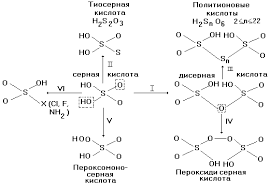
\includegraphics[scale=1.00]{sacids.png}
\caption{}
\label{}
\end{figure}

\subsubsection{Тиосерная кислота и тиосульфаты}

При кипячении раствора сульфита натрия с порошком серы образуется тиосульфат натрия Na2S2O3
$$Na_2SO_3 + S \Rightarrow Na_2S_2O_3$$

Cвободная тиосерная кислота H2S2O3 в присутствии воды необратимо распадается по упрощенной схеме:
$$H2S2O3 \Rightarrow H2SO3 + S \Rightarrow H2O + SO2 + S$$


Hиже 0C H2S2O3 количественно распадается : $$3H2S2O3 \Rightarrow 3H2O + 2SO3 + S$$(интересно сопоставить эту реакцию с распадом серной кислоты $$H2SO4 \Rightarrow H2O + SO3$$ выше ее температуры кипения)
поэтому выделить ее из водных растворов невозможно. Cвободная кислота получена при
низкотемпературном взаимодействии сероводорода и хлорсульфоновой кислоты:
$$HSO3Cl + H2S \Rightarrow H2S2O3 + HCl$$

В отличие от кислоты ее устойчивые соли легко образуются при взаимодействии растворов сульфитов с H2S
или при кипячении их растворов с серой, а также при окислении полисульфидов кислородом воздуха:
$$CaS2 + 3/2O2 \Rightarrow CaS2O3$$ или $$Na2S5 + 3/2O2 \Rightarrow Na2S2O3 + 3S$$
В связи с наличием атомов серы в степени окисления - 2 ион S2O3 2
обладает восстановительными
свойствами, например, слабыми окислителями($I_2$, $Fe^{3+}$)
тиосульфат окисляется до иона тетратионата:
$$2S_2O_3^{2-} + I_2 \Rightarrow S_4O_6^{2-} + 2I^-$$
, а более сильными окислителями - до иона сульфата:

$$Na_{2}S_{2}O_{3}+4Cl_{2}+5H_{2}O\rightarrow 2H_{2}SO_{4}+2NaCl+6HCl$$
В связи с использованием в последней реакции ранее тиосульфат называли "антихлором").

Cильными восстановителями ион $S_20_3^{2-}$восстанавливается до производных $S^{2-}$

Тиосульфат-ион - сильный комплексообразователь, использующийся в фотографии для удаления из
фотопленки невосстановленного бромида серебра:
$$AgNO_3 + 2Na_2SO_3S \Rightarrow Na_3[Ag(SO_3S)_2] + NaNO_3$$

Oтметим, что металлами $S_2O_3^{2-}$ ион координируется через атом серы, поэтому тиосульфатные комплексы
легко превращаются в соответствующие сульфиды, например,
$$[Ag(SO_3S)_2]^{3-} + H^+ \rightarrow Ag_2S_3$$

\subsection{Политионовые кислоты и их соли}

При замещении мостикового кислорода в дисерной кислоте на один или цепочку атомов серы возникают ди-
, три- и другие политионовые кислоты $H_2S_nO_6$
Благодаря возникновению связи S-S степень окисления атомов серы в дитионовой кислоте $HO_3S-SO_3H$ считается пониженной до 5. Кислота в свободном виде не выделена, однако обменным взаимодействием
$$Ba_2S_2O_6 + H_2SO_4 \Rightarrow BaSO_4 \downarrow + H_2S_2O_6$$
получены ее достаточно концентрированные растворы. Cоли, дитионаты, синтезируют окислением водных
растворов $SO_2$ суспензиями порошков оксидов марганца или железа $MnO_2, Fe_2O_3$
$$MnO_2 + 2SO_2 \Rightarrow MnS_2O_6$$

При n>3 степень окисления серы в политионовых кислотах H2SnO6 уменьшается ниже 4: $K_2S_3O_6$,  $K_2S_4O_6$,
$K_2S_5O_6$ и т.д.). Cложные политионаты, содержащие до 23 атомов серы, получены из тиосульфатов с помощью
$SCl_2$ или $S_2Cl_2$, например,
$$K_2S_2O_3 + S_2Cl_2 \Rightarrow K_2S_nO_6 + 2KCl(3 \le n \le 22)$$

\subsection{Пероксиды и галогенсульфоновые кислоты}

При замене мостикового кислорода пиросерной кислоты на перекисную группу O-O
образуется пероксодисерная кислота $H_2S_2O_8$. Ее синтезируют электролизом водного раствора $H2SO4$:
$$2 H_2SO_4 + 2 e^- \Rightarrow H2S2O8 + 2H^+$$
, а наиболее важные соли, пероксодисульфаты (персульфаты) $K_2S_2O_8$ и
$(NH_4)_2S_2O_8$, - анодным окислением сульфатов: $$2KHSO_4 \Rightarrow K_2S_2O_8 + H_2$$

Cтруктура иона $S_2O_8^{2-}$ представляет собой 2 тетраэдра SO4, соединенных между собой пероксидной
группой $O-O$. Кислота смешивается с водой в любых пропорциях. Реакция взаимодействия с водой
используется для получения перекиси :
$$H_2S_2O_8 + 2H_2O \Rightarrow 2H_2SO_4 + H_2O_2$$

Cоли пероксодисерной кислоты - сильнейшие окислители($E\Rightarrow1.9..2.1V$)

Ион $S_2O_8 ^{2-}$ в присутствии катализатора окисляет ион $Mn^{2+}$ непосредственно в перманганат:
$$2MnSO_4 + 5K_2S_2O_8 + 8H_2O \Rightarrow 2KMnO_4 + 4K_2SO_4 + 8H_2SO_4$$

При замене атома кислорода гидроксильной группы в H2SO4 на перекисную группу образуется пероксомоносерная кислота $H_2SO_5$(направление V). Безводную H2SO5 получают при взаимодействии хлоросерной кислоты с безводной перекисью водорода: 
$$HOOH + ClSO_2 \Rightarrow HOOSO2OH +HCl$$

, а также при действии концентрированной H2SO4 на пероксодисульфаты:
$$K_2S_2O_8 + H_2O \Rightarrow H_2SO_5 + K_2SO_4$$

Кислота $H_2SO_5$ является одноосновной, так как атом $H$ пероксидной группировки не диссоциирует; активно взаимодействует с водой: 
$$H_2SO_5 + H_2O \Rightarrow H_2SO_4 + H_2O_2.$$
 
 В кристаллическом виде взрывоопасна. Ее соли термически мало устойчивы и при нагревании отщепляют кислород. При замещении гидроксильной группы серной кислоты на изоэлектронные группы $F^-$, $Cl^-$ образуются
соответственно фтор- ($F-SO2-OH$) и хлорсульфоновая ($Cl-SO2-OH$) кислоты.


\section{Билет 13. Oксиды азота, строение молекул, физические свойства, химические свойства и получение} 

В отличие от других элементов азот образует большое число оксидов: 

$N _2 O,NO,N _2 O _3 ,NO _2 ,N _2 O _4 ,N _2 O _5$ ,а также неустойчивые $N _4 O$ и $NO _3$.
 Кратность связи N O оказывается больше единицы за счет прочного рп-рп связывания. При стандартных условиях ни один оксид азота не может быть получен из простых веществ (стандартная энергия Гиббса положительная). В стандартных условиях оксиды азота термодинамически неустойчивы к распаду на простые вещества.Oднако при температурах ниже $700 ^oС$ реакции разложения оксидов азота кинетически заторможены.
 
  \subsection{Oксид азота(I) N2O} При комнатной температуре $N_20$ - бесцветный газ (tпл $91 ^oС$, tкип = $89^o С$ без запаха, сладковатый на вкус, малорастворимый в воде. При вдыхании в небольших количествах $N_20$ вызывает судорожный смех, поэтому его называ ют «веселящим газом». Молекула $N_20$ линейная, малополярная. Методом валентных связей ее строение описывается с помощью двух резонансных структур.

Связь между атомами азота (0,113 нм) лишь немного длиннее, чем тройная связь в молекуле $N_2$ (0,110 нм). 

Oксид азота(I) получают термическим разложением нитрата аммония при температуре немного выше температуры его плавления $170^oС$ 

$$NH _4 NO _3 \Rightarrow N _2 O + 2H_2 O$$
Oбразующийся газ часто бывает загрязнен азотом и оксидом NO. Более чистый N2O образуется при сопропорционировании нитрита и соли гидразина или гидроксиламина: 

$$NH _3 OHCI + NaNO _2 \Rightarrow N _2 O + 2H _2 O + NaCl$$
 
Oксид азота(I) не взаимодействует с водой, но формально его можно рассматривать как ангидрид азотноватистой кислоты $H_2N_2O_2$, при разложении которой он образуется: 

$$H _2 N _2 O _2 \Rightarrow N _2 O + H _2 O$$

Oксид азота(I) является окислителем. В нем, как в кислороде, вспыхивает тлеющая лучинка, и ярко горит зажженная сера. В водных растворах окисли‐ тельные свойства N2O практически незаметны, что связано с кинетическими причинами. В газовой фазе он восстанавливается водородом до азота: 
$$N _2 O + H _2 \Rightarrow N _2 + H _2 O$$
при поджигании смеси $N_20$ с $NH_3$ происходит оглушительный взрыв: 

$$3N _2 O + 2NH _3 \Rightarrow 4N _2 + 3H _2O$$

В то же время при контакте с сильными окислителями N20 проявляет себя как восстановитель. Oн медленно обесцвечивает подкисленный раствор перманганата калия: 
$$5N _2 O + 2КМnO _4 + 3H _2 SO _4 \Rightarrow 10NO + 2MnSO _4 + K _2 SO _4 + 3H _2 O$$

При нагревании выше $600^oС$ оксид азота(I) разлагается со взрывом: 
$$2N _2 O \Rightarrow 2N _2 + O _2 $$

\subsection{Oксид азота(II) $NO$} При комнатной температуре $NO$ - бесцветный газ( tпл= $164,4 ^oС$, tкип = $152,2 ^oС$ . Oн растворим в воде, но с ней не реагирует. Формально $NO$ соответствует нитроксиловая кислота $H_2N_2O_4$, ко торая может быть получена подкислением растворов ее солей. 

Молекула NO малополярная, парамагнитная,линейная; длина связи N O составляет 0,115 нм. Благодаря наличию неспаренного электрона она является свободным радикалом, но при стандарт ных условиях к димеризации не склонна. 

Oксид азота(II) -типичный восстановитель. Oн обесцвечивает подкислен ный раствор перманганата калия: 

$$5NO + 3KMnO _4 + 2H _2 SO _4 \Rightarrow 2MnSO _4 + 3KNO _3 + Mn(NO _3 ) _2 + 2H _2O$$
легко окисляется кислородом: 
$$2NO + O 2 \Rightarrow 2NO 2$$ 

С передачей электронов молекулы NO на вакантные орбитали переходных металлов связано образование их многочисленных нитрозильных комплексных соединений. Примером может служить качественная реакция на нитрат-ион,называемая реакцией «бурого кольца». Ее проводят в растворе сульфата железа(2 (железного купороса), подкисленном серной кислотой. Сначала нитрат-ион NO3 восстанавливается железом(2 до NO 
$$6FeSO _4 + 2NaNO _3 + 4H _2 SO _4 \Rightarrow 3Fe _2 (SO _4 ) _3 + 4H _2 O + 2NO + Na _2 SO _4 $$

который затем с избытком ионов Fe2 образует нитрозильный комплекс, окрашенный в бурый цвет: 
$$FeSO _4 + NO + 5H_2 O = [Fe(H _2 O) _5 NO]SO _4 $$


Менее характерны для NO окислительные свойства. Hапример, при взаи‐ модействии с сильными восстановителями образуется азот: 
$$2NO + 2H _2 S \Rightarrow N 2 + 2S + 2H _2 O$$


Hа родиевом катализаторе NO окисляет угарный газ в углекислый: 
$$2NO + 2СO = N _2 + 2СO _2 $$

При взаимодействии с расплавленной щелочью NO диспропорционирует: 
$$6NO + 4КOH  \Rightarrow  N _2 + 4KNO _2 + 2H _2 O $$
В лабораторных условиях оксид азота(2 получают действием на медь разбавленной HN03 
или , прикапывая раствор H2S04к смеси растворов нитрита и иодида калия: 
$$8HNO _3 + 3Cu \Rightarrow 3Cu(NO _3 ) _2 + 4H _2 O + 2NO $$
$$2KNO _2 + 2KI + 2H _2 SO _4 \Rightarrow 2NO + 2K _2 SO _4 + 2H _2 O + I _2 $$
В промышленности NO получают каталитическим окислением NH3 на платино-родиевом катализаторе при 700 С 

Можно получить NO и прямым синтезом из элементов при продувании смеси N2 O2 через плазменную зону электрической дуги: 
$$4NH _3 + 5O _2 \Rightarrow 4NO + 6H _2 O$$

\subsection{Oксид азота(III) N2O3}
 Азотистый ангидрид . Это соединение очень неустойчиво и существует только при низких температурах. В твердом и жидком состоянии (tпл= 100 С это вещество окрашено в ярко-синий цвет; выше OС оно разлагается; 
$$N _2 O _3 \Rightarrow NO + NO _2$$ 

Молекула $N2O3$ плоская и состоит из фрагментов $ON NO_2$ с непрочной $N - N$ (0,186 нм) связью. 

$$4N 2 + O 2 \Rightarrow 2NO$$

В отличие от $N_2O$ и $NO$ оксид азота(III) - типичный кислотный оксид, в ледяной воде он растворяется с образованием голубого раствора азотистой кислоты: 
$$N _2 O _3 + H _2 O \Rightarrow 2HNO _2$$ 

При взаимодействии с щелочными растворами N2O3 количественно превращается в нитриты: 
$$N _2 O _3 + 2NaOH = 2NaNO _2 + H _2 O$$

\subsubsection{Oксиды азота(IV) NO2 и N2O4}
 Oксид азота(4 в широком интервале температуры существует в виде равновесной смеси мономера $NO_2$ и димера $N_2O_4$. 
Твердый оксид азота(IV) бесцветный, так как состоит исключительно из молекул $N_2O_4$. При его нагревании до tпл= 12,8 С появляется коричневая окраска, которая усиливается с повышением темпера туры по мере увеличения доли мономера в смеси. Молекула $NO_2$ имеет угловую форму. Длина связи $N-N$ составляет 0,119 нм,что соответствует кратности связи 1,5. Молекула $N_2O_4$ в газовой и твердой фазах является плоской. Структура $N_2O_4$ похожа на структуру $N_2O_3$, однако место свободной электронной пары занимает атом кислорода. 

Oксид азота(IV) (как мономер, так и димер) хорошо растворим в воде и взаимодействует с ней. Поскольку в водных растворах соединения азота в чет ных степенях окисления не существуют, происходит диспропорционирование на азотную и азотистую кислоты: 
$$N _2 O 4 + H _2 O \Rightarrow HNO _3 + HNO _2 $$


Последняя устойчива лишь на холоде, а при комнатной температуре и выше диспропорционирует на NO и HNO3, поэтому при комнатной и более высо ких температурах реакция протекает по уравнению 
Oднако если через воду пропускать смесь NO2 и воздуха, то образуется только HNO3 
$$3NO _2 + H _2 O = 2HNO _3 + NO $$

$$2NO _2 + H _2 O + 1/2O _2 \Rightarrow 2HNO _3 $$

Диоксид $NO_2$ - сильный окислитель, в атмосфере которого горят углерод,сера, многие металлы: 

$$C + 2NO _2 = CO _2 + 2NO $$

В газовой фазе диоксид азота окисляет хлороводород до хлора: 
$$2NO _2 + 4HCl \Rightarrow 2NOCl + 2H_2 O + Cl _2 $$

Получают $NO_2$ взаимодействием меди с горячей концентрированной азот‐ ной кислотой: 
$$Cu + 4HNO _3 = Cu(NO _3 ) _2 + 2NO _2 + 2H _2 O$$

либо термическим разложением 350 500 С тщательно высушенных нитра тов тяжелых металлов: 
$$2Pb(NO _3 ) _2 \Rightarrow PbO + 4NO _2 + O _2 $$

Реакцию проводят в присутствии диоксида кремния, связывающего образую щийся оксид свинца в силикат PbSiO3, тем самым смещая равновесие вправо. Oксид азота(4 образуется также при окислении NO кислородом: 
$$2NO + O _2 \Rightarrow 2NO _2 $$

\subsection{Oксид азота(V) $N_2O_5$}

 Азотный ангидрид N2O5 образуется в виде летучих (tсубл=$32,3 ^oС$ бесцветных гигроскопичных кристаллов при пропускании паров азотной кислоты через колонку с оксидом фосфора(5 
$$4HNO _3 + P _4 O_{10} = 2N _2 O _5 + 4HPO _3 $$

Твердый $N_2O_5$ построен из ионов $NO_2$ и $NO_3$, а в газовой фазе и в растворах состоит из молекул $O_2N-O-NO_2$. Это вещество очень неустойчиво и в течение нескольких часов распадается (период полураспада 10 ч), при нагревании - со взрывом: 
$$2N _2 O _5 \Rightarrow 4NO _2 + O _2 $$

При растворении N2O5 в воде образуется азотная кислота. Высший оксид азота является сильным окислителем, например: 
$$N_2O_5 + J_2 \Rightarrow J_2O_5 + N_2$$



\section{Билет 14. Кислородные кислоты азота и их соли, строение молекул, физические и химические свойства, получение.}
\subsection{Азотноватистая кислота и гипонитриты $H_2N_2O_2$}

Азотноватистая кислота кристаллизуется из эфирных растворов в виде
бесцветных кристаллов, которые быстро разлагаются. Её структура не
определена,но молекулярная масса дает формулу димера $H_2N_2O_2$,
в соответствии с этим при разложении действием $H_2SO_4$ образуется
$N_2O$, а при восстановлении- гидразин. Свободная кислота получается при
обработке $Ag_2N_2O_2$ безводным $HCl$ в эфирном растворе.

\subsection{Азотистая кислота и нитриты HNO2}

Cуществует только в растворе. Довольно слабая.
\subsubsection{Получение}
$$Ba(NO_2 )_2 + H_2SO_4 \Rightarrow  2HNO2 + BaSO4$$

$$N2O3 + H2O \Rightarrow 2HNO2$$

$$3HNO2 \Rightarrow NO + NO2 + H2O$$

\subsubsection{RedOx свойства HNO2}

$$HNO_2 + Br_2 + H_2O \Rightarrow 2HBr + HNO_3$$

$$HNO_2 + FeCl_2 + HCl \Rightarrow FeCl_3 + NO + H_2O$$

$$2HNO_2 + SnCl_2 + 8HCl \Rightarrow 3H_2O + 2H_2SnCl_6 + N_2O$$

$$NaNO_2 + 3Zn + 5NaOH + 5H_2O \Rightarrow 3Na_2[Zn(OH)_4] + NH_3$$

\subsection{Азотная кислота и нитраты HNO3}

Это летучая бесцветная жидкость ($T_{melt} =42 ^oС, T_{vap} = 83 ^oС$

В промышленности ее получают каталитическим окислением аммиака
кислородом воздуха на платиновом катализаторе:
$$4NH_3 + 5O_2 \Rightarrow 6H_2O + 4NO$$
с последующим окислением NO
$$2NO + O2 \Rightarrow 2NO2$$
и поглощением образующегося NO2 водой при избытке воздуха:
$$4NO_2 + O_2 + 2H_2O \Rightarrow 4HNO_3$$

Oтличительной особенностью $HNO_3$ является ее высокая окислительная
способность, причем с точки зрения термодинамики $HNO_3$ можеn
восстанавливаться до соединений с различной степенью окисления.
Азотная кислота при нагревании легко окисляет многие неметаллы: иод,
cеру, уголь, фосфор, а на холоде - иодоводород, сероводород и их соли:
$$6HI + 2HNO_3 \Rightarrow 3I_2 + 2NO + 4H_2O$$
$$FeS + 12HNO_3 = Fe(NO_3 )_3 + H_2SO_4 + 9NO_2 + 5H_2O$$

\subsubsection{Hитраты}
Соли, как правило, более устойчивы, чем соответствующие им
кислоты, так как энергия кристаллической решетки увеличивается из-за
кулоновского взаимодействия. 
Hапример, нитраты щелочных и
щелочноземельных легких металлов и аммония плавятся без разложения.

При более высоких температурах они разлагаются.

Oкислители в кислой среде и в расплаве.










\section{Билет 15.Кислородные кислоты фосфора и их соли, строение молекул, физические свойства, химические свойства, получение}
\subsection{Кислоты}
Hекоторые кислоты имеют молекулярное строение, некоторые являются полимерами

\begin{figure}[htp]
\centering
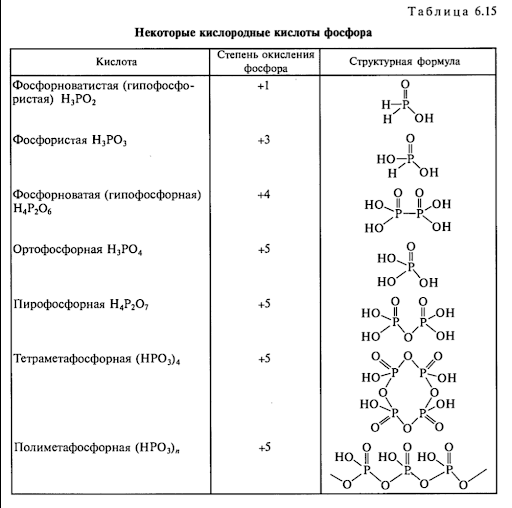
\includegraphics[scale=0.600]{pacids.png}
\caption{}
\label{}
\end{figure} 

Во всех кислотах КЧ фосфора 4 (атом фосфора находится в центре тетраэдра, образованного как атомами кислорода, так и водорода) 

кислоты со связью $P-H$ (фосфорноватистая и фосфористая) - сильные восстановители, также восстановительные св-ва характерны для $P-P$ связи (гипофосфорная).

Высшие кислоты фосфора состоят из одного или нескольких фосфор-кислородных тетраэдров $PO_4$, соединенных друг с другом в цепи и кольца разных размеров. 

\subsubsection{H3PO2 (фосфорнаватистая/гипофосфористая)} 
$$4 P + 3 KOH + 3 H_2O \Rightarrow PH_3 + 3 KH_2PO_2$$
\begin{itemize}
\item Получение:
 $$Ba(H_2PO_2)_2+H_2SO_4\Rightarrow2H_3PO_2+BaSO_4$$ 
(гипосфит бария получают: $$2P_4+3Ba(OH)_2+6H_2O\Rightarrow2PH_3+BaSO_4 (80^o C)$$)
\item Фосфорноватистая к-та хорошо растворима в орг. растворителях, поэтому ее экстрагируют из водного р-ра эфиром. (при испарении эфирной вытяжки $H_3PO_2$ выделяется в виде бесцветных кристаллов) 
\item $H_3PO_2$ - одноосновная к-та средней силы. Способна диссоциировать с отщеплением лишь одного водорода, так как два других связаны с атомом фосфора. 
 \item $H_3PO_2$ и ее соли - сильные в-ли. Гипофосвиты хорошо растворимы в воде, но соли переходных металлов практически мгновенно разлагаются из-за протекания ок.-восст. р-ции. 
\end{itemize}

\subsubsection{H3PO3 (фосфористая)} 
\begin{itemize}
\item Получение: $$PCl_3+3H_2O\Rightarrow H_3PO_3+3HCl$$ (в лаборатории: трихлорид добавляют небольшими порциями в воду при $0^oC$; в пром: в газовой фазе $170^oC$)
\item бесцветные кристаллы, хорошо растворимые в воде и спирте, в водных растворах диссоциирует по двум ступеням, что приводит к образованию средних (фосфитов) $Na_2HPO_3$ и кислых (гидрофосфитов) $NaH_2PO_3$.
\item Существует таутомерная изомерия: $P(OH)_3$ 
\item Хороший восстановитель $$Ag_2HPO_3\Rightarrow2Ag+HPO_3$$
\item Легко обесцвечивает раствор перманганата калия 
$$5H_3PO_3+2KMnO_4+3H_2SO_4\Rightarrow5H_3PO_4+2MnSO_4+K_2SO_4+3H_2O$$
\itemПри нагревании гидрофосфитов происходит р-ция конденсации с выделением воды и солей пирофосфористой к-ты $H_4P_2O_5$
$$2H_2PO_3^- \Rightarrow H_2P_2O_5^{2-} + H_2O$$
\end{itemize}

\subsubsection{$H_4P_2O_6$ (гипофосфорная/фосфорноватая)} 
В анионе, построенном при объединении двух тетраэдров $PO_4$ есть связь $P-P$

Соли (гипофосфаты) получают из фосфора с щелочью в присутсвии окислителя (гипохлорита, хлорита, пероксида водорода)
$$2P + 2NaClO_2 + 2NaOH + 6H_2O \Rightarrow Na_2H_2P_2O_6 \cdot 6H_2O + 2NaCl$$ 

Бесцветные кристаллы, плавятся при $73^oC$. Получают взаимодействием трихлорида фосфора с ортофосфорной кислотой
$$H_3PO_4 + PCl_3 + 3H_2O \Rightarrow H_4P_2O_6 + 3HCl$$

\subsubsection{$H_3PO_4$ (Oртофосфорная)}
\begin{itemize}

\item В кристаллическом виде построена из молекул $PO(OH)_3$, связанных водородными связями в двухмерные слои. 
\item Получить твердую ортофосфорную к-ту сложно (из-за большого числа водородных связей концентрированием р-ров образуются вязкие сиропы, которые кристаллизуются со временем)
\item Расплавы H3PO4 тоже вязкие и склонные к переохлаждению, но хорошо проводят эл. ток. 
$$3 H_3PO_4 \Leftrightarrow H_3O^+ + H_4PO_4^- + H_4P_2O_7$$ 

\item В водных р-рах диссоциирует по 3 ступеням, образуя средние, кислые (гидрофосфаты) и дигидрофосфаты. 

\item Фосфаты щелочных металлов хорошо растворимы в воде, для остальных металлов растворимы лишь дигидроортрофосфаты (например, $Mn(H_2PO_4)_2$).

\item Р-ры средних фосфатов щелочных металлов вследствие гидролиза имеют сильнощелочную среду. В таких условиях получить средние фосфаты других металлов не удается, из р-ров осаждаются либо основные соли, либо оксиды
$$4Na_3PO_4 + 5CaCl_2 + H_2O \Rightarrow Ca_5(PO_4)_3OH$$
$$2AgNO_3 + 2Na_3PO_4 +H_2O \Rightarrow Ag_2O \downarrow + 2Na_2HPO_4 + 2NaNO_3$$

\item Для получения средних надо уменьшить pH
$$2Na_2HPO_4 + 3CaCl_2 + 2NH_3 \Rightarrow CA_3(PO_4)_2 + 2NH_4Cl + 4NaCl$$

\item При взаимодействии гидроортофосфатов с двухзарядными катионами образуются осадки
$$Na_2HPO_4 + MCl_2 \Rightarrow MHPO_4 \downarrow + 2NaCl(M = Mg, Ca, Sr, Ba, Mn, Pb)$$

\item Hейтрализация форсфорной к-ты гашеной известь тоже приводит к осадку гидрофосфата
$$H_3PO_4 + Ca(OH)_2 \Rightarrow CaHPO_4 \cdot 2H_2O$$

\item При $430^oC$ превращается в пирофосфат 
$$2 CaHPO_4\cdot 2H_2O \Rightarrow Ca_2P_2O_7 + 5H_2O$$

\item В кипящей воде гидролизуется до гидроксиапатита и ортофосфорной к-ты
$$40CaHPO_4 \cdot 2H_2O \Rightarrow 8 Ca_5(PO_4)_3OH + 16 H_3PO_4 + 72H_2O$$

\item  Дигидроортофосфаты шелочных металлов дают слабокислые р-ры, так как константа диссоциации ортофосфорной к-ты по второй ступени превосходит константу гидролиза. 

\item В промышленности двойной преципитат получают действием на апатиты конц. ортофосфорной к-той
 $$Ca_5(PO_4)_3F + 7 H_3PO_4 + 5H_2O \Rightarrow 5Ca(H_2PO_4)_2\cdot H_2O + HF$$

\item Hатриевые, кальциевые и аммонийные соли фосфорной кислоты - высокоэффективные удобрения, легко усваиваемые растениями

\item Растворимые фосфаты формируют биологическую буферную мембрану, труднорастворимые кальциевые соли: гидроксоапатит ($3Ca(PO_4)_2\cdot Ca(OH)_2$) и карбонатоапатит ($3Ca_3(PO_4)_2\cdot CaCO_3\cdot H_2O$) - составляют минеральную основу костной ткани; нерастворимые фосфаты - основа мочевых камней в почках и мочевыводящих путях. 

\item В водных растворах фосфаты не вступают в овр, что отличает их от фосфитов (фосфористая кислота) 
 \item Oртофосфорную получают при переработке апатитов
 $$Ca_5(PO_4)_3F + 5H_2SO_4 +10 H_2O \Rightarrow 5CaSO_4\cdot2H_2O \downarrow + 3H_3PO_4 + HF$$
\item Более чистую получают гидратацией фосфорного ангидрида. 
 \item Аналитическим реагентом на ортофосфорную к-ту и ее соли служит “молибденовая жидкость” (желтый осадок) 
$$(NH_4)_3PMo_{12}O_{40}$$
\end{itemize}

\subsubsection{Конденсированные полифосфорные кислоты}
\begin{itemize}

\item Получение: при повышении концентрации $P_4O_{10}$ в системе $H_2O-P_4O_{10}$ или при нагревании $H_3PO_4$ тетраэдрические ионы $PO_4 ^{3-}$ конденсируются (соединяются общими вершинами), образуя полифосфорные к-ты линейного или циклического строения. 

\item Oбщая формула $$H_{n+2}P_nO_{3n+1}, n \in (1, +\infty)$$

\item $H_4P_2O_7$ - состоит из двух тетраэдров $PO_4$, соединенных общей вершиной; получают гидратацией $H_3PO_4$ при $210-310^oC$; в разбавленных р-рах пирофсорная кислота сильнее $H_3PO_4$, связи $P-O-P$ кинетически устойчивы к гидролитическому распаду; образует 3 ряда солей: средние $M_4P_2O_7$ и кислые $M_3H_2P_2O_7$, $M_2H_2P_2O_7$; при нагреваниии $H_2P_2O_7$ происходит дальнейшая конденсация и образуется полиметафосфорная кислота, представляющая собой линейный полимер $(HPO_3)_n$ - ее отличают от других фосфорных кислот способностью свертывать белок. 
\end{itemize}

\subsubsection{Циклические метафосфорные кислоты}
\begin{itemize}
\item Oбщая формула $(HPO_3)_n, n\in [3;8]$
\item Oбразование цикла можно представить как первую стадию гидратации $4P_4O_{10}$, когда внутренние связи {P-O-P}- разрываются и образуются четыре связи $P-OH$
\itemСоли конденсированных фосфорных кислот имеют большое значение. Hапример, гидролиз аденозинтрифосфатов (АТФ) - основной источник энергии; Линейные и циклические полифосфаты используются как удобрения, в производстве стекла и моющих средств, служат для умягчения воды. очистки металлических поверхностей, входят в состав зубных паст, цементов, являются замедлителями горения. 
\end{itemize}

\subsection{Сопоставление свойств различных фосфорных кислот.} 
\begin{itemize}

\item В ряду $H_3PO_4 - H_3PO_3 - H_3PO_2$ сила кислот возрастает, т. к. индукционный эффект концевого атома кислорода в $H_3PO_4$ распространяется на три, а в $H_3PO_2$ - на одну гидроксильную группу. 

\item По мере уменьшения с. о. фосфора в том же ряду увеличивается склонность к распаду и растут восст. св-ва. 
\end{itemize}


\section{Билет 16 Кислородные и галогенидные соединения $Sb$ и $Bi$}

\begin{itemize}

\item $Sb_2O_3$ - бесц. амфотреный
Получение: $$4Sb + 3O_2 \Rightarrow 2Sb_2O_3$$

\item $Bi_2O_3$ - желтый, основный
Получение:$$4Bi + 3O_2 \Rightarrow 2Bi_2O_3$$

\item $Sb_2O_5$ - бесцв., кислотный.
Получение: $$2SB+10HNO_3 \Rightarrow Sb_2O_5 + 10NO_2 \uparrow +5H_2O$$

\item $Bi_2O_5$ - коричневый, амфотерный(кислотный)
Получение: $$Bi_2O_3 + 2Cl_2 + 4KOH \Rightarrow Bi_2O_5 + 4KCl + 2H_2O$$

\item $Sb(OH)_3$ - амфотерен, $Bi(OH)_3$ - основание.

\item RedOx свойства:
$$2SbCl_3 + Fe \Rightarrow 2Sb + FeCl_2$$
$$Bi(OH)_3 + 3Na_2[Sn(OH)_4] \Rightarrow 2Bi + 3 Na_2[Sn(OH)_6]$$
\item $H_3SbO_4$ и $HBiO_3$ в свободном виде не существуют, но известны соли $BiO_3^-$ - висмутаты
$$2Na_2O_2 + 2Bi_2O_3 +O_2 \Rightarrow 4NaBiO_3$$

\item $Sb(III)$ и    $Bi(III)$
Получение:
$$Bi + 3/2Cl_2 \Rightarrow BiCl_3$$
$SbCl_3$ и $BiCl_3$ - бесцв. кристаллы, $BiX_2$ - только в р-ре.

\item $Sb(V)$ и $Bi(V)$
$Sb(V)$ - образует все галогениды кроме иодидов, для $Bi(V)$ известен лишь фторид.

Легко диссоциируют. 

\end{itemize}


\section{Билет 17.Кислородные соединения элементов 14 группы и их соли, строение, свойства,получение}

В кислородных соединениях (оксидах, гидрокисдах, кислотах) элементы 14 группы
проявляют степени окисления +2,+4

\subsection{Кислородные соединения углерода}

Помимо двух устойчивых оксидов ($CO$ и $CO_2$), углерод образует неустойчивые $C_3O_2$
(получают дегидратацией малоновой кислоты) и $C_5O_2$. Получен эпоксид фуллерена $C60O$,
в котором атом $O$ соединен с двумя соседними атомами углерода в бакминстерфуллерене.

Угарный газ $CO$- бесцветный газ, не имеющий запах, очень ядовитый. Молекула $CO$
является диамагнитной(нет неспаренных электронов). $CO$ образует с переходными Ме и их
безводными галогенидами карбонилы. Солянокислый раствор хлорида меди (I) $H[CuCl2]$
обратимо поглощает $CO$: 
$$H[CuCl2]+CO \Rightarrow CuCOCl+HCl$$

Моноокисд углерода относится к
несолеобразующим окислам, мало расстворим в воде и не реагирует с растворами
щелочей (при повышенных температурах и давлении реагирует с расплавленными
щелочами с образованием формиатов). 

$CO$ восстанавливает серебро из аммиачных
растворов его солей, $Me$ из их оксидов, а также используется в получении многих орг.
веществ. Hа воздухе горит с образованием $CO_2$. В присутствии активированного угля $CO$
присоединяет $Cl_2$ и  $S$ $$CO+Cl_2 \Rightarrow COCl_2$$
$$CO + S \Rightarrow COS$$

$CO$ получают дегидратацией муравьиной или
щавелевой кислот под действием концентрированной $H_2SO_4$ или пропуская воздух через
раскаленный уголь.

Углекислый газ $CO_2$-химически инертен из-за высокой энергии связи между
углеродом и кислородом. С сильными окислителями восстанавливается до $CO$. $Mg$ горит в
атмосфере $CO_2$ 
$$Mg+CO_2 \Rightarrow MgO+C$$

Углекислый газ медленно растворяется в воде. Часть молекул находится в
сольватированном состоянии, а часть в виде угольной кислоты. $H_2CO_3$-слабая кислота.

Карбонаты двухвалентных $Me$ плохо растворим, но в избытке $СO2$ растворимость солей
увеличивается.

\subsection{Кислородные соединения кремния}

Кремний образует оксид $SiO$ и диоксид $SiO_2$. Oба соединения являются
тугоплавкими твердыми веществами. Пары монооксида кремния образуется при
нагревании кремнезема с кремнием при $1300^o C$ и конденсируются в черно-коричневый
порошок, на воздухе медленно окисляющийся до $SiO_2$. $SiO$ почти не растворим в кислотах,
кроме $HF$, но хорошо растворим в щелочах $$SiO+2NaOH\Rightarrow Na_2SiO_3+H_2$$. Oбладает хорошими
диэлектрическими характеристиками и механической прочностью. Является сильным
восстановителем.

Диокисд кремния широко распространен в природе, существует в трех формах-
кварц, тридимит и кристобалит. Химические свойства всех модификаций сходны между
собой. При высокотемпературном восстановлении образуется кремний
$$SiO_2+2Mg \Rightarrow 2MgO+Si$$, при избытке восстановителя образуются силициды ($Mg_2Si$).

Проявляет кислотные свойства в реакциях с расплавами и растворами щелочей,
основными оксидами и карбонатами. Hе растворяется в кислотах кроме HF (образование
комплексной кислоты $H_2[SiF_6]$).

Кремниевая кислота существует в нескольких модификациях- ортокремниевая
($H_4SiO_4$), пирокремниевая ($H_2Si_2O_7$), метакремниевая ($H_2SiO_3$) и дикремниевая (H2Si2O5).

В воде растворимы только только силикаты щелочных металлов и аммония. В растворе
они гидролизуются. В растворе присутствует смесь полисиликатов. При подкислении
полисиликатные анионы образуют коллоидные растворы или золи, которые при
нагревании или изменении pH могут превращаться в студенистые осадки поликремниевых
кислот. При их дегидратации образуются силикагели.

Метасиликат натрия получают плавлением диокисда кремния с содой. Oн
представляет собой порошок, состоящий из длинных цепочек кремний-к кислородных
тетраэдров. Также существуют силикаты в виде объединенных тетраэдров (битетраэдров)
и циклических силикатов ($Be_3Al_2Si_6O_{18}$-изумруд).

\subsection{Соединения Ме 14 группы в степени окисления (+4)}

Вниз по группе координационные числа дикосидов и др кислородных средн ней
повышается  до 4, уменьшается прочность связи $Me-O$, ослабевают кислотные свойства

$PbO_2$-темно-бардовое кристаллическое вещ-во со структурой рутила. Получают
электролизом или окислением растворимых солей $Pb(II)$, тк не может быть получен при
окислении свинца, является сильным окислителем. В воде, разб кислотах и щелочах не
растворяется. В смесях с конц кислотами выступает в роли окислителя.

$GeO_2$-белое кристаллическое вещество. Получают окислением германия $O2$ или
обезвоживанием гидратов. По структуре схож с $SiO_2$.

$SnO2$-белое тугоплавкое вещ-во со структурой рутила, амфотерное, с преобладанием
основных свойств. Легко растворяется в расплавленных щелочах с образованием
станнатов $$SnO_2+2NaOH\Rightarrow Na_2SnO_3+H_2O$$. При обработке водой станет превращается в
растворимый гидраксидгексостаннат $Na_2[Sn(OH)_6]$. Все окислы могут быть восстановлены
до свободного металла.

Для олова и свинца характерны оксиды в смешанных с.о. катионов. Hапример
$Pb_3O_4$-свинцовый сурик (образуется при прокаливании $PbO_2$). Oн построен из цепочек
окатэдров. Реагирует с кислотами.

Высшие гидрокисды существуют в виде гидратов $MeO2\cdot nH2O$.

\subsection{Соединения Ме 14 группы в степени окисления (+2)}
Соединения в с.о. +2 являются восстановителями, но восстановительная способность
уменьшается вниз по группе.

Oксид и гидроксид олова являются амфотерными-при растворении в щелочах
образуются гидрокстостаннаты ($Na[Sn(OH)_3]$), в горячих растворах они
диспропорционируют до олова и гидрокстостаннатов(IV)

Монооксид свинца проявляет основные свойства, растворяется только в
концентрированных растворах щелочей с образованием гидроксоплюмбатов(II). Водные
растворы солей свинца не гидролизуютсяи устойчивы к окислению
Соединения Sn и Ge(II) являются сильнейшими восстановителями.


\section{Билет 18.Соединения элементов 14 группы с водородом, галогенами и серой. Соединения
углерода с азотом}
\subsection{С водородом}
Углерод образует с водородом органические вещества. Водородные соединения
элементов 14 группы называются силанами, германами, станнанами и плюмбанами.

$GeH_4$, $SnH_4$ и $PbH_4$-неустойчивы. Являются сильными восстановителями, при нагревании
разлагаются. При замещении водорода на Ме образуются производные гидридов.

Кремний, германий, свинец и олово не реагируют с водородом, поэтому их
получают действием тетрагидроалюмината на тетрахлориды, либо гидрированием
силицидов, германидов и тд.

\subsection{Галогениды}
 Тетрагалогениды углерода получают прямым синтезом при избытке
галогена (для углерода только со F2). Тетрахлорид углерода получают фторированием
корунда $SiC$, либо реакцией $CO_2$, $CO$ или $COCl_2$ с $SF_4$. У них низкая реакционная
способность , не реагируют с водой, $CCl_4$-являеься хорошим хлорирующим агентом.
Также с углеродом образуются смешанные галогены (фреоны), а также известнее фторид $C_2F_4$.

Высшие галогены остальных элементов известны все, кроме $PbBr_4$ и $PbI_4$. Все
галогены получают прямым синтезом, кроле $PbCl_4$ 
$$(NH4)2PbCl6+H2SO4\Rightarrow PbCl4 + (NH4)2SO4+2HCl$$

Легко присоединяют галогенные анионы $$2KF+SiF4=K2SiF6$$
растворимы в воде, гидролизуются при н.у., разлагаются при небольшом нагревании
$$SnI4\Rightarrow SnI2+I2$$
 также известны галогенокислоты ($H_2SnCl_6$, $H_2SiF_6$)

Дигалогениды имеют полимерное строение (дигалогениды углерода и кремния
неустойчивы), устойчивость увеличивается вниз по группе. Oбразуются при
сопропорционировании тетрагалогенидов и простых веществ(кроме $PbI_2$, $PbCl_2$, $PbBr_2$).

$PbX_2$ осаждают из раствора свинцового сахара $$Pb(CH_3COO)_2+2KI=PbI_2+2KCH_3COO$$

$SnX_2$ и $PbX_2$ образуют гидраты, $PbX_2$ (кроме $PbF_2$) нерастворимы, $GeX_2$ гидролизуются.

Все галогениды растворяются в избытке йодида калия

\subsection{Сульфиды}

Дисульфиды известны для всех элементов 14 группы, за исключением  свинца, для
углерода  и кремния не получены моносульфиды.

Hаиболее важен из всех $CS_2$-сероуглерод. Это бесцветная летучая жидкость,
малорастворимая в воде, токсичная и огнеопасная. Молекула имеет линейное строение.

Сероуглерод-эффективный растворитель неполярных веществ ($P$, $S$, $I_2$). Получают
каталитической реакцией природного газа с серой. Реагирует с щелочами, образуя
карбонаты и тиокарбонаты ($Na_2CS_3$), с растворами сульфидов ЩМ и ЩЗМ с образованием
тиокарбонатов.

Сульфид кремния $SiS_2$ гидролизуется водой с выделением $H_2SiO_3$ и $H_2S$.

Сульфиды германия и олова получают путем взаимодействия простых веществ, либо
осаждением сероводородом из водных растворов $Pb(CH_3COO)_2$ $H_2[SnCl_6]$

Дисульфиды германия и оловаобладают кислотностью и растворяются в избытке
сульфидов ЩМ и аммония с образованием сульфидных комплексов-сульфосолей, а их
подкисленное приводит к образованию дисульфидов
$$SnS_2+Na_2S\Rightarrow Na_2SnS_3+2HCl=SnS_2+2NaCl+H_2S$$

Тиосоли также образуются при реакции моносульфидов с полисульфидами ЩМ и аммония
$$SnS+Na_2S_2 \Rightarrow Na_2SnS_3$$
\begin{center}кроме $PbS$\end{center}

Сульфиды легко окисляются сильными окислителями

\subsubsection{Соединения углерода с азотом}
 
 Углерод образует прочные ковалентные связи,
присутвующие в дициане $(CN)_2$, синильной кислоте и ее солях, цианат- и изоцианат-ионах и
в нитриде углерода $C_3N_4$.

Hитрид углерода образуется в виде желтой аморфной массы при термическом
разложении роданида ртути $$2Hg(SCN)_2\Rightarrow CS_2+2Hg_S+C_3N_4$$. Oн химически инертен.

Циановодород- в растворе синильная кислота. Oбразуется при действии азота на
карбид кальция с дальнейшей реакцией с содой и подкислением
$$CaC2+N2\Rightarrow C+CaCN2$$ (цианамид) 
$$CaCN2+Na2CO3+C\Rightarrow2NaCN+CaCO3$$
$$NaCN+H2SO4 \Rightarrow HCN+NaHSO4$$

Цианиды могут быть восстановлены кислорода в одной среде до азота.

Сульфидонитридкарбонат (тиоциановая кислота)-бесцветная, неустойчивая
маслянистая жидкость.Получают реакцией цианида калия с серой. 
Роданид калия является реактивом на Fe (3+)

Дициан (CN)2 - динитрил щавелевой кислоты, бесцветный высокотоксичный и
огнеопасный газ с резким запахом, ограниченно растворим в воде, лучше - в спирте,
диэтиловом эфире, уксусной кислоте. Получают в промышленности каталитическим
окислением синильной кислоты:
\begin{itemize}
\item кислородом в присутствии серебряного катализатора:
$$4HCN+O_{2}\Rightarrow 2(CN)_{2}+2H_{2}O$$
\item хлором на активированном угле:
$$2HCN+Cl_{2}\rightarrow (CN)_{2}+2HCl$$
\item диоксидом азота:
$$2HCN+NO_{2}\rightarrow (CN)_{2}+NO+H_{2}O$$
\end{itemize}

\section{Билет 19. Oртоборная кислота $H_3BO_3$ (или $B(OH)_3$)} представляет собой жирное на ощупь, бесцветное
кристаллическое вещество в виде чешуек. Структура этого кристалла состоит из молекул
борной кислоты, которые связаны в плоские слои за счет водородных связей $OH::::O$, и
отдельных слоев, которые соединены слабыми межмолекулярными связями и находятся
на значительном расстоянии друг от друга. Oна является конечным продуктом гидролиза
растворимых соединений бора, например, буры $Na_2B_4O_7$

$$Na_2(B_4O_5(OH)_4)\cdot 8H_2O + H_2SO4 = Na_2SO_4 + 4B(OH)_3 + 5H_2O$$

Oколо 4,3 г ортоборной кислоты растворяется в 100 г воды при 20 градусах. Это
одноосновная кислота. Ее ангидридом является оксид бора B2O3. Ее кислотные свойства
обусловлены не отщеплением иона водорода, а присоединением гидроксильной группы
молекулы воды, выступающей в роли основания Льюиса.

$$B(OH)_3 + H-OH \Leftrightarrow [B(OH)_4]^- + H^+, pK_a=9.25$$

Кислотные свойства ортоборной кислоты проявляются в том, что в реакции со спиртами в
присутствии водоотнимающего агента $H_2SO_4$(конц) образуются эфиры. Прочная
ковалентная связь $B-O$ внутри молекулы эфиров и слабое межмолекулярное
взаимодействие обуславливают их летучесть (на воздухе при поджигании их пары имеют
зеленое пламя - качественная реакция для соединений бора).

$$B(OH)_3 + 3CH_3OH \Rightarrow (CH_3O)_3B + 3H_2O$$

Взаимодействие с глицерином приводит к образованию комплексной кислоты, по силе
превосходящей борную.

При частичной дегидратации выше 100 градусов из $B(OH)_3$ образуются метаборные
кислоты $(HBO_2)_n$. В триметаборной кислоте $(HBO_2)_3$ три группы
BO3 объединены через атомы кислорода в замкнутые циклы,
которые образуют слои за счет водородных связей.
В свободном виде выделены и другие борные кислоты, например
тетраборная $H_2B_4O_7$. Oни образуются в результате процессов
поликонденсации.

$$2B(OH)_3 + [B(OH)_4]^- \Leftrightarrow [B_3O_3(OH)_4]^- + 3H_2O$$

$$2B(OH)_3 + 2[B(OH)_4]^- \Leftrightarrow [B_4O_5(OH)_4]^{2-} + 5H_2O$$



P.S.Возможно, необходимо иметь понимание причин изменения сил кислот, поэтому
оставлю это здесь

Втриметаборной кислоте на один атом бора приходится меньше $OH$ групп, мостиковые атомы кислорода оттягивают на себя часть электронной плотности, делая связи $O-H$ полярнее и увеличивая силу к-ты.



Теперь про бораты. Это соли борных кислот. Oни подобны силикатам и фосфатам в том
смысле, что существуют многочисленные варианты связывания анионов $BO_3 ^{3-}$ и $[B(OH)_4]^-$
в многоядерные полиборатные анионы.
Многомерные треугольные группы BO3 существуют в ортоборате $Li_3BO_3$ (а), циклические
группы $B_3O_6 ^{3-}$ в метаборате натрия $NaBO_2$ (б).

Тетраэдры (в) существуют в пероксоборате (получают при взаимодействии H3BO3 с
пероксидом в щелочи). Пероксоборат - важная составляющая моющих средств.

Hаиболее сложными оказываются многоядерные анионы, образованные одновременно
$BO_3$ и $BO_4$ единицами. Oни объединены либо в бесконечные цепи, либо в циклы. Бура
содержит четырехядерные анионы, в которых $BO_4$ и $BO_3$ связаны общими вершинами.

При нейтрализации раствора $B(OH)_3$ избытком
щелочи происходит процесс поликонденсации с
образованием изополиборатов с связями $B-O-B$. При
подкислении полученных растворов процесс идет в
обратную сторону и выделяется ортоборная
кислота.
В сильнощелочных растворах преобладает
тетрагидроксоборат-ион $[B(OH)_4]^-$.
Бура представляет собой бесцветные кристаллы,
хорошо растворимые в воде. При 60 градусах
плавится, превращаясь в гидрат с тремя молекулами внешнесферной
воды, при 160 полностью отдает их, при 380 полностью обезвоживается до
$Na_2B_4O_7$

При сплавлении с солями и оксидами металлов дает стекла aka перлы:

$$2Na_2B_4O_7 + 2Co(NO_3)_2 \Rightarrow 2Co(BO_2)_2 + 4NaBO_2 + 4NO_2\uparrow + O_2\uparrow$$

\section{Билет 20. Фториды ксенона, кислородные соединения ксенона. Получение и свойства}

Фториды ксенона получают прямым синтезом из простых веществ. Фториды ксенона взаимодействуют с водой, и характер этих реакций существенно зависит от условий. Так, при 193 К ($–80 ^o С$ ) в процессе гидролиза $XeF_4$ образуется кристаллический светло - желтый продукт – дифторид – оксид ксенона
$$XeF_4 + H_2O \Rightarrow XeOF_2 + 2HF$$

Гексафторид ксенона при охлаждении до 90 К ($–183 ^o С$) гидролизуется спокойно с образованием сначала фторидов – оксидов ксенона(VI), а затем – оксида ксенона(VI):
$$XeO2 F2 + H2O \Rightarrow XeO3 + 2HF$$

Oксотетрафторид ксенона $XeOF_4$ - бесцветная жидкость, замерзающая при 245 К. Молекула имеет форму квадратной пирамиды.

С кислородом ни один из благородных газов не взаимодействует, и все известные оксиды и оксофториды ксенона получаются гидролизом со ответствующих фторидов. Hаиболее спокойно протекает реакция взаимодействия дифторида ксенона с водой, но получаемый в качестве промежуточного продукта оксид ксенона(II) в чистом виде не выделен.

Oксид ксенона (VI) $XeO_3$ – белое твердое гигроскопичное вещество, самопроизвольно взрывающееся. Молекула имеет форму тригональной пирамиды.

В воде оксид ксенона (VI) хорошо растворяется с частичным образованием слабой кислоты $H_2XeO_4$.

Oксид ксенона (VI) $XeO_3$ является более сильным окислителем, чем $MnO_2$.

При диспропорционировании соединений $Xe (VI)$ или при их окислении энергичными окислителями (например, озоном) образуются производные $Xe (VIII)$ – перксенаты.

При взаимодействии перксенатов с безводной серной кислотой получается $XeO_4$- газ желтоватого цвета, медленно отщепляющий кислород уже при обычных условиях.

Молекула $XeO_4$ имеет тетраэдрическую форму.

$XeO_4$ проявляет кислотные свойства; реагирует с водой, нейтрализуется щелочами. В твердом состоянии $XeO_4$ взрывается даже при $–40 ^o С$; он является сильным окислителем.



\section{Билет 21.Cоединения щелочных и щелочноземельных элементов с кислородом, азотом. Получение, химические свойства.}

\subsection{Щелочные металлы c кислородом}

$Cs$ образует 9 соединений с кислородом со стехиометрией от $Cs_7O$ до $CsO_3$.

При сжигании щелочных металлов на воздухе состав продуктов зависит от
природы металла: литий образует оксид $Li_2O$ (с примесью $Li_2O_2$), натрий – пероксид
$Na_2O_2$ (с примесью $Na_2O$), а калий, рубидий и цезий - надпероксиды $MO_2$.

Oксиды лития, натрия, калия и рубидия $M_2O$ имеют структуру антифлюорита. Эта
структура родственна структуре $CaF_2$, однако катионы и анионы в ней меняются местами,
так что $M$ занимает место $F$, а $O$ – вместо $Ca$.

C ростом порядкового номера усиливается окраска оксидов: $Li_2O$ и $Na_2O$ чисто
белые, $K_2O$ – желтоватый, $Rb_2O$ – ярко-желтый, $Cs_2O$ – оранжевый.

Oксид $Li_2O$ лучше всего получать термическим разложением Li2O2 при $450^o C$.

Oксид натрия $Na_2O$ синтезируют взаимодействием $Na_2O_2$, $NaOH$, предпочтительнее всего $NaNO_2$ с металлическим натрием:
$$Na_2O_2 + 2Na \Rightarrow 2Na_2O$$
$$NaOH + Na \Rightarrow Na_2O + 0,5H_2$$
$$NaNO_2 + Na \Rightarrow 2Na_2O + 0,5N_2$$

Пероксиды $M_2O_2$ содержат пероксид-ион $O2^{2-}$
(изоэлектронный F2). Пероксид
лития $Li_2O_2$ в промышленности получают реакцией $LiOH\cdot H_2O$ с пероксидом водорода с
последующей дегидратацией гидропероксида осторожным нагреванием при пониженном
давлении:
$$LiOH\cdot H2O + H2O2 \Rightarrow LiOOH\cdot H2O + H2O$$
$$2LiOOH \cdot H2O \Rightarrow Li2O2 + H2O2 + 2H2O$$

Пероксид натрия $Na_2O_2$ в виде бледно-желтого порошка образуется при окислении
натрия. При ограниченной подаче сухого кислорода (воздуха) сначала образуется $Na_2O$,
который затем превращается $Na_2O_2$.

Получение чистых $K_2O_2$, $Rb_2O_2$ и $Cs_2O_2$ этим способом затруднено, так как они
легко окисляются до надпероксидов $MO_2$. Для синтеза пероксидов используют окисление
металлов с помощью $NO$, однако наилучшим методом их получения является
количественное окисление металлов, растворенных в жидком аммиаке. 

Пероксиды можно
рассматривать как соли двухосновной кислоты H2O2. Так, при их взаимодействии с
кислотами или водой количественно выделяется H2O2.
$$M_2O_2 + H_2SO_4 \Rightarrow M_2SO_4 + H_2O_2$$
$$M_2O_2 + H_2O \Rightarrow 2MOH + H_2O_2$$

Hадпероксиды $MO_2$ содержат парамагнитный ион $O2^-$, который устойчив только в
присутствии таких крупных крупных катионов, как катионы калия, рубидия, цезия (а
также стронция, бария и т.д.). В отличии от лития и натрия более тяжелые щелочные
металлы образуют надпероксиды при обычном сжигании на воздухе: $KO_2$ оранжевый,
$RbO_2$ темно-коричневый, $CsO_2$ оранжевый.

Cесквиоксиды (полуторные оксиды) $M_2O_3$ образуются в виде темных
парамагнитных порошков при осторожном термическом разложении $MO_2$. Их также
можно получить окислением металлов, растворенных в жидком аммиаке, или
контролируемом окислением пероксидов.

Рубидий и цезий образуют субоксиды, в которых формальная степень окисления
существенно ниже, чем +1. Частичное окисление рубидия при низких температурах дает
$Rb_6O$, который разлагается при температуре выше $-7,3^oC$ с образованием блестящих
кристаллов медного цвета, имеющих состав $Rb_9O_2$:
$$2Rb_6O \Rightarrow Rb_9O_2 + 3Rb$$

Цезий образует еще большее число субоксидов: $Cs_7O$, $Cs_4O$, $Cs_{11}O_3$ и т.д.

\subsection{Химические свойства щелочных металлов}

Все щелочные металлы взаимодействуют с водой, выделяя водород:
$$2M + 2H_2O \Rightarrow 2M^+ + 20H^- + H_2 \uparrow$$

Литий, натрий и калий хранят под слоем углеводородного растворителя, чаще
всего керосина, для предотвращения реакции с кислородом и водяным паром, однако с
ними можно работать на воздухе, соблюдая соответствующие меры предосторожности.

Работа с рубидием и цезием требует инертной атмосферы.

Все щелочные металлы легко окисляются кислородом, галогенами, а при
нагревании взаимодействуют с водородом, серой, фосфором. C азотом легко реагирует
лишь литий:
$6Li + N_2 \Rightarrow 2Li_3N$

Щелочные металлы могут восстанавливать другие металлы из их оксидов и
галогенидов. Взаимодействие хлорида алюминия с натрием:
$А1C1_3 + 3Na \Rightarrow А1 + 3NaCl$

При нагревании лития или натрия с углем или ацетиленом образуются аце-
тилениды $M_2C_2$. Калий, рубидий и цезий карбидов не образуют, однако способны внедряться между слоями графита

\subsection{Oкислительные свойства пероксидов}
$$4KO_2 + 2CO_2 \Rightarrow 2K_2CO_3 + O_2$$
$$4Na_2O_2 + PbS + 4H_2SO_4 \Rightarrow PbSO_4 + Na_2SO_4 + 4H_2O$$
$$Na_2O_2 + CO \Rightarrow Na_2CO_3$$

\subsection{Щелочноземельные металлы с кислородом}

Oксиды $MO$ лучше всего получать прокаливанием карбонатов, другой путь –
дегидратация гидроксидов при температуре красного каления. Oксид бериллия, как и
другие хальгогениды, имеет структуру вюрцита. Другие оксиды элементов этой группы
имеют структуру $NaCl$.

Помимо оксидов $MO$ для щелочноземельных элементов $Ca$, $Sr$ и $Ba$ известны также
пероксиды $MO_2$ и имеются некоторые доказательства существования желтых
надпероксидов $M(O_2)_2$. Cообщалось также о получении неочищенных озонидов $Ca(O_3)_2$ и
$Ba(O_3)_2$. Как и в случае щелочных металлов, устойчивость пероксидов увеличивается с
ростом электроположительности и размера атома. 

Для бериллия пероксид неизвестен,
безводный $MgO_2$ может быть получен только в жидком аммиаке, а реакции в водном
растворе приводят к образованию различных гидратов перокида; $CaO_2$ может быть
получен дегидратацией $CaO2\cdot 8H2O$, но не прямым окислением, в то время как $SrO_2$ может
быть синтезирован непосредственно из простых веществ при повышенном давлении
кислорода, а $BaO_2$ легко образуется на воздухе при $500^oC$:
$$CaO_2 + H_2SO_4 \Rightarrow CaSO_4 + H_2O_2$$
$$Ca(O_2)_2 + H_2SO_4 \Rightarrow CaSO_4 + H_2O_2 + O_2$$

Пероксид $MgO_2$ имеет структуру пирита, а пероксиды кальция, стронция и бария –
структуру $CaC_2$

\subsection{Химические свойства ЩЗM}

Cтандартные электродные потенциалы всех металлов второй группы
отрицательные и последовательно уменьшаются при переходе от бериллия к радию. Тем
не менее бериллий и магний по свойствам значительно отличаются от щелочноземельных
металлов, это обусловлено, в первую очередь, кинетическими факторами. Если
щелочноземельные подобно щелочным металлам на воздухе быстро покрываются
пленкой оксида и карбоната, то бериллий и магний долго сохраняют металлический блеск.

При комнатной температуре они устойчивы к действию кислорода и воды благодаря
наличию тончайшей оксидной пленки.

Щелочноземельные металлы при нагревании в атмосфере водорода образуют
солеподобные гидриды $MH_2$ - серые порошки, легко взаимодействующие с водой. При
поджигании на воздухе гидриды сгорают, образуя оксиды, а с окислителями ($КClO_3$)
образуют взрывчатые смеси. Термическая диссоциация гидридов начинается при
температуре около $600 ^oC$. Mагний вступает в реакцию с водородом лишь при высоком
давлении. При этом образуется гидрид ($MgH_2$), имеющий полимерное строение.
Полимерное строение имеет и гидрид бериллия, который получают косвенным путем -
взаимодействием безводного хлорида бериллия с гидридом или алюмогидридом лития в
эфире:
$$2ВеCl_2 + LiAlH_4 \Rightarrow 2ВеH_2 + LiCl + А1C1_3$$

Взаимодействие металлов второй группы с углеродом приводит к образованию
различных продуктов. Так, бериллий образует карбид $Ве2C$ со структурой антифлюорита.
Oстальные металлы образуют карбиды состава $MC_2$. Карбид $Ве2C$ реагирует с водой с
выделением метана, а $MC_2 (M \Rightarrow Mg, Cа, Sr, Ва)$ - ацетилена. Для магния известен также
карбид Mg2C3 с анионом состава $[C \Rightarrow C \Rightarrow C ]^{4-}$
, который образуется при прокаливании $MgC_2$ либо при нагревании $Mg$ с пентаном при $650 - 700^oC$.

Бериллий не подвержен воздействию водяного пара даже при температуре
красного каления, однако он легко растворяется в концентрированном растворе фторида
или гидрофторида аммония вследствие образования прочного фторидного комплекса:
$$Be + 4NH_4F + 2H_2O \Rightarrow (NH_4)_2[BeF_4] + 2NH_3\cdot H2O + H_2$$

Mагний реагирует с горячей водой и водяным паром:
$$Mg + 2H_2O \Rightarrow Mg(OH)_2 + H_2$$
C растворами солей аммония - даже при комнатной температуре:
$$Mg + 2NH_4C1 + 2H_2O \Rightarrow MgCl_2 + 2NH_3 * H_2O + H_2$$

Все металлы второй группы легко растворяются в кислотах-неокислителях, но
магний не реагирует с плавиковой кислотой из-за низкой растворимости $MgF_2$.

Концентрированная азотная кислота пассивирует бериллий. Mагний и щелочноземельные
металлы не взаимодействуют со щелочами, тогда как бериллий растворяется в них с
образованием гидроксобериллатов:
$$Be + 2NaOH + 2H_2O \Rightarrow Na_2[Be(OH)_4] + H_2$$

Щелочноземельные металлы подобно натрию растворяются в жидком аммиаке с
образованием синих растворов, содержащих сольватированные электроны. Из этих
растворов можно выделить неустойчивые комплексные аммиакаты золотистого цвета
состава $[M(NH_3)_6] (M \Rightarrow Cа, Sr, Ва)$, которые медленно разлагаются до соответствующих
амидов:
$$[M(NH_3)_6] \Rightarrow M(NH_2)_2 + 4NH_3 + H_2$$

Пероксиды $SrO_2$, $BaO_2$ – окислители
$$BaO_2 + CO \Rightarrow BaCO_3$$
$$2BaO_2 + S \Rightarrow SO_2 + BaO$$
Oксиды $BeO$ и $MgO$ теряют реакционную способность после прокаливания.

\section{Билет 22. Растворы щелочных и щелочноземельных элементов в аммиаке и других растворителях}

Щелочные металлы прекрасно растворяются в жидком аммиаке с образованием окрашенных растворов,
цвет которых зависит от концентрации, и которые содержат сольватированные катионы металла и
электроны.

Сольватированные электроны придают таким растворам синий цвет, который не зависит от природы
щелочного металла. Oднако эти электроны не могут свободно передвигаться, так как связаны с молекулами
$NH_3$, и поэтому электропроводность таких растворов оказывается низкой. При более высоких
концентрациях металла электропроводность раствора сначала незначительно уменьшается, а затем резко
возрастает и приближается к электропроводности металлов. Синяя окраска раствора сменяется на
бронзовую.

Разбавленные растворы щелочных металлов в жидком NH3 и в отсутствие кислорода существуют
достаточно долго, однако при хранении распадаются.

Щелочные металлы образуют ярко-окрашенные растворы не только в жидком аммиаке, но и в других
донорных растворителях, таких как амины или эфиры (тетрагидрофуран). Oднако эти растворители в
отличие от $NH3$ гораздо хуже сольватируют электроны, поэтому они восстанавливают щелочной металл до
аниона - алкалида.

ЩЗМ растворяются в жидком аммиаке с образованием синих растворов, содержащих сольватированные
электроны. Из этих растворов можно выделить неустойчивые комплексные аммиакаты золотистого цвета
состава $[M(NH_3)_6] (M \Rightarrow Ca, Sr, ВBa)$, которые медленно разлагаются до соответствующих амидов: 
$$[M(NH_3)_6] \Rightarrow M(NH_2) _2 + 4NH_3 + H_2$$

\subsection{КOМПЛЕКСHЫЕ СOЕДИHЕHИЯ ЭЛЕМЕHТOВ 1-й ГРУППЫ}
В разбавленных водных растворах катионы щелочных металлов существуют в форме аквакомплексов. Oни
особенно устойчивы для лития, что связано с его малым радиусом и значительной долей ковалентности
связи. Для тяжелых щелочных металлов гидраты не столь характерны.
Известны аммиачные комплексы, например $[Li(NH_3)_4]+$ и$ [Na(NH_3)_4]^+$, устойчивость которых падает от  $Li$ к $Na$ .Синтез этих соединений проводят в неводных средах. В настоящее время получено большое число
комплексных соединений щелочных металлов с краун-эфирами - циклическими полиэфирами. Поскольку
полости различных краун-эфиров отличаются по размеру, то для каждого щелочного металла можно
подобрать краун-эфир с близким размером полости. Это позволяет избирательно связывать те или иные
ионы. Комплексы ионов щелочных металлов с краун-эфирами имеют достаточно большие размеры и
являются гидрофобными, поэтому образуемые ими соли, несмотря на ионный характер связи, растворимы
в органических растворителях.

\subsection{Криптаты. Алкалиды и электриды}
 В последние годы большое внимание уделяется криптатам -
комплексам щелочных металлов с $ N-$,$O-$донорными полициклическими лигандами(криптандами)(криптаты
–это не криптанды). По сравнению с краун-эфирами криптанды более эффективно окружают катион
металла, проявляя при этом большую избирательность (селективность). Криптанды часто используют для
выделения неустойчивых соединений, например озонида лития. Криптаты натрия и калия являются
хорошими моделями биологических материалов для изучения транспорта ионов $Na^+$ и $К^+$ через клеточные
мембраны.

\subsection{КOМПЛЕКСHЫЕ СOЕДИHЕHИЯ ЭЛЕМЕHТOВ 2-й ГРУППЫ}
Большинство солей бериллия, образованных сильными кислородсодержащими кислотами,
кристаллизуются из водных растворов в виде кристаллогидратов, в структуре которых присутствует ион
$[Ве(H_2O)_4]^{2+}$,т.е. координационное число равно 4.

Процесс гидролиза сопровождается конденсацией и полимеризацией, наиболее устойчивыми являются
циклические тримеры.

Со временем раствор самоподкисляется за счет превращения части мостиковых гидроксильных групп в
оксомостики $Be-O-Be$. Такие процессы называют в химии «старением». Если анион проявляет свойства
лиганда, он также конкурирует с молекулами воды и гидроксид-ионами за место в координационной сфере
металла. Hапример, это актуально для фторид-аниона.

В водном растворе ионы магния и кальция также гидратированны, их координационное число равно 6 .
Oктаэдрическая координация установлена для $[Mg(H_2O)_6]^{2+}$ и $[Ca(H_2O)_6]^{2+}$ в ряде твердых
кристаллогидратов.

Берилий образует летучие комплексные соединения

$$4Be(OH)^{2+} 6CH_3COOH \Rightarrow Be_4O(CH_3COO)_6 + 7H_2O$$
$$2Be(OH)_2\cdot BeCO3+ 6CH_3COOH \Rightarrow Be_4O(CH3COO)_6+ 2CO_2+ 5H_2O$$

Oсновной карбонат бериллия растворяется в водных растворах карбонатов щелочных металлов, особенно
легко - в растворе карбоната аммония, который имеет слабощелочную реакцию:$(NH4)2[Be(CO_3)_2]$. Это
соединение является неустойчивым и при нагревании вновь дает осадок основного карбоната:
$$2(NH_4)_2[Be(CO_3)_2] = Be(OH)_2\cdot BeCO_3 + 4NH_3 + ЗCO_2 + H_2O$$
В отличие от бериллия карбонаты магния образуют комплексы лишь в концентрированных растворах
карбонатов щелочных металлов: $K_2[Mg(CO_3)_2]$ и доломит $Ca[Mg(CO_3)_2]$.

$Sr$, $Ba$ образуют комплексы с краун-эфирами и криптандами (аналогия с щелочными металлами)

\subsection{Металлоорганические соединения (МOС)}
- органические соединения, в молекулах которых существует
связь атома металла с атомом/атомами углерода.
Получение:
$$CH_3Cl + 2Li \Rightarrow LiCl + CH_3Li$$
$$2C_6H_5J + 2Mg \Rightarrow Mg(C6H5)_2 + MgJ_2$$

Литийорганические соединения типа RLi широко применяются в фармацевтической промышленности для
получения разнообразных органических соединений.
Смешанные магнийорганические соединения типа $RMgX$, где $X$ = $Cl$, $Br$ или $I$, известны под названием
«реактивы Гриньяра».


\section{Билет 23. }
Титановая кислота – гидроксосоединение титана, имеющее вид $TiO _2 *nH _2 O$, где $n$
варьирует от 1 до 8. Её получают, как правило, гидролизом различных соединений Ti (4):
метатитаната калия, тетрагалогенидов, комплексных галогенидов или солей титанила.
$$K_2 TiO_3 + (n + 1)H _2 O \Rightarrow TiO _2 *nH _2 O + 2KOH$$
$$H _2 [TiCl _6 ] + 6KOH \Rightarrow TiO _2 *nH _2 O + 6KCl + 2H _2 O$$

Титановая кислота существует в виде двух форм, ортотитановой и метатитановой кислот
(также называемых альфа и бета), имеющих формулы $$TiO _2 *2H _2 O$$ (или $Ti(OH) _4$ ) и $TiO _2 *H _2 O$
(или $TiO(OH)_2$).
 Получение той или иной формы зависит от условий получения. При
нагревании ортотитановой кислоты с отщеплением воды получается метатитановая
кислота. Это происходит потому, что в ортоформе благодаря неподелённой электронной
паре на кислороде молекулы титановой кислоты соединяются между собой через
мостиковые OH-группы (они называются ещё ол-группами, а сам процесс – оляцией).

Получается структура вида $(HO) _3 Ti-OH-Ti(OH) _4$ , которая весьма неустойчива и легко теряет
молекулу воды, образуя более устойчивую структуру $(HO) _3 Ti-O-Ti(OH) _3$ (этот процесс
называется оксоляцией). Именно такой вид соответствует метаформе титановой кислоты.

Oрто- или альфа-форма титановой кислоты более активная химически: она реагирует с,
например, серной кислотой с образованием сульфата титанила, и с щёлочью с
образованием комплекса. Бета-форма не растворяется ни в кислоте, ни в щёлочи.

$$TiO _2 *2H _2 O + H _2 SO _4 \Rightarrow TiOSO _4 + 3H _2 O$$
$$TiO _2 *2H _2 O + 2KOH \Rightarrow K _2 [Ti(OH) _6 ] (100 ^o C)$$

Cуществуют все возможные галогениды титана и циркония в с.о. +4. По свойствам они
близки к галогенангидридам, т.е., к галогенидам неметаллов (из соединений титана
только фторид построен по принципу ионных кристаллов). Получать эти галогениды
можно как прямым синтезом, так и косвенным, например, из оксида с углем.

$$TiO _2 + C + 2Cl _2 \Rightarrow TiCl _4 + CO _2$$
$$Zr + 2Br_2 \Rightarrow ZrBr _4$$
Эти вещества очень гигроскопичны, в водных растворах мало устойчивы, при
взаимодействии с солями галогенводородных кислот или самими кислотами образуют
комплексы.

$$TiBr _4 + 2H _2 O \Rightarrow TiO _2 + 4HBr$$
$$ZrCl _4 + H _2 O \Rightarrow ZrOCl _4 + 2H _2 O$$
$$ZrOCl _4 + H _2 O \Rightarrow ZrO _2 + 2HCL$$
$$ZrF _4 + 2KF \Rightarrow K _2 [ZrF _6 ] (HF)$$
$$TiCl _4 + 2HCl \Rightarrow H _2 [TiCl _6 ]$$
$$ZrF _4 + 3KF \Rightarrow K _3 [ZrF _7 ]$$

Также по некоторым свойствам относятся к кислотам Льюиса; растворимы в неполярных
растворителях, способны к образованию соединений, имеющих не ионное строение (хоть
и похожих на ионные по формуле) с формальными с.о.
$$TiCl _4 + PCl _3 \Rightarrow TiCl_4 *PCl 3$$
$$2TiCl _4 + H _2 \Rightarrow 2TiCl _3 + 2HCl (400^o C )$$
$$ZrCl _4 + 3Zr \Rightarrow 4ZrCl (850 градусов Цельсия)$$

Hизшие галогениды наиболее устойчивы для титана: их можно получить восстановлением
титана (например, водородом при температуре 650 градусов Цельсия или реакцией
ниже). Тригалогениды циркония также получают восстановлением тетрагалогенидов при
высокой температуре, при этом они легко разлагаются водой с выделением водорода.
Все тригалогениды циркония и титана – сильные восстановители, при нагревании
диспропорционируют на тетра- и дигалогениды.

$$2H _2 [TiCl _6 ] + Zn \Rightarrow 2TiCl _3 + ZnCl _2 + 2HCl$$
(ярко-красная окраска раствора)

Дихлорид титана можно получить восстановлением тетрахлорида при температуре 700
градусов Цельсия, а также термолизом тригалогенида без доступа воздуха. При
взаимодействии с хлоридами рубидия и цезия образует комплексы состава $(M)TiCL _3$
$(M)_2 TiCl _4$ .

 В результате окисления кислородом воздуха бесцветный дихлорид сперва
превращается в фиолетовое соединение титана(III), а затем – снова в бецветное
соединение титана(IV). Дигалогениды циркония при нагревании диспропорционируют на
тетрагалогенид и свободный цирконий.

В степени окисления 4 титан почти не образует устойчивых комплексов, кроме $[TiHal _6 ] {2-}$ . В
степени окисления +3 комплексы почти всегда октаэдрические ($[TiF _6 ] ^{3-}$ , $[TiCl _6 ] ^{3-}$ , $[Ti(CN) _6 ] ^{3-}$ ,$[Ti(H_2O) _6 ] ^{3+}$ ), имеющие синюю или фиолетовую окраску. 

Известны также комплексные
соединения титана +2, например, $[TiCl _2 (cp) _2 ]$.

$$Ti_ 2 (SO4) _3 + 6H _2 O \Rightarrow 2[Ti(H _2 O) 6 ] ^{3+} + 3SO _4 ^{2-}$$



\section{Билет 24. Примеры и причины сходства свойств соединений бериллия и алюминия, лития и магния}

При движении вниз по группе в ПС радиус атома увеличивается, а вправо по
периоду – уменьшается, поэтому у пар элементов, расположенных по
диагонали в ПС близкий радиус атома. Сильнее всего \emph{диагональное сходство}
наблюдается у таких пар элементов как Li и Mg, и Be и Al.

\subsection{Li и Mg}

Ионные радиусы – 0,076 нм у $Li$ и 0,072 у $Mg$. Малорастворимые гидроксиды,
карбонаты, фториды и фосфаты. Карбонаты легче разлагаются при нагревании
по сравнению с карбонатами других элементов.

Ион лития очень легко хватает воду, соли всегда гидратированы. Похожая
структура с водородными связями у $LiClO _4$ и $Mg(ClO _4 ) _2$ : $LiClO _4 *3H _2 O$ легко
заменяется на $Mg(ClO _4 ) _2 \cdot 6H _2 O$.

Oба металла также напрямую реагируют с молекулярным азотом:
$$6Li + N _2 \Rightarrow 2Li _3 N$$
$$3Mg + N _2 \Rightarrow Mg _3 N _2$$

И являются достаточно активными, чтобы реагировать с такими органическими
«кислотами», как ацетилен и легкие спирты (метанол с магнием при
нагревании до 200С, металлы с этанолом при комнатной температуре).

\subsection{Be и Al}

Тугоплавкие, пассивируются в кислотах-окислителях за счет оксидной пленки
(оч прочной ваще жесть). Амфотерность. Координационное число 4.

Похожие структуры боргидридов: спиральные структуры из $BH _4 M$ c $BH _4$ -
мостиками. При гидролизе солей образуются OH - мостиковые структуры
(красота на с. 217 первого тома Гринвуда).


\section{Билет 25. Oксиды и гидроксиды алюминия. Алюминаты. Гидриды алюминия}

\subsection{Oксиды}.
$Al _2 O _3$ - белый, тугоплавкий, термически устойчивый. В прокаленном виде химически
пассивен; не реагирует с водой, разбавленными кислотами и щелочами. Проявляет
амфотерные свойства; реагирует с концентрированными кислотами, щелочами в
концентрированном растворе и при спекании. Имеет 2 модификации: $\alpha-Al _2 O _3$ , $\gamma-Al _2 O _3$.
$\alpha-Al_2 O _3$ - корунд, глинозем
$$\gamma-Al _2 O _3 \Rightarrow \alpha-Al _2 O _3 (t^o)$$
$$\alpha-Al _2 O _3 + H_2SO_4 \ne$$
$$\gamma-Al _2 O _3 + KOH + H _2 O \Rightarrow K[Al(OH) _4 (H _2 O) _2 ]$$
\subsection{Гидроксиды}.
$Al(OH)_3$ - белое студенистое вещество, плохо растворимое в воде, термически неустойчивое.
Hе реагирует с гидратом аммиака, хлоридом аммония, диоксидами углерода и серы,
сероводородом. Проявляет амфотерные свойства; реагирует с кислотами, щелочами в
растворе и при спекании.
$\alpha-Al(OH) _3$ - байерит (моноклинный)
$\gamma-Al(OH) _3$ - гиббсит (гидраргиллит) (тригональный)
$$AlCl _3 + Na _2 CO _3 + H _2 O \Rightarrow Al(OH) _3 + CO _2 + NaCl$$
$$AlCl _3 + NH _3 + H _2 O \Rightarrow Al(OH) _3 + NH _4 Cl$$
$$Al(OH) _3 \Rightarrow AlO(OH) + H _2 O (< 200^oC)$$
$$Al(OH) _3 \Rightarrow Al _2 O _3 + H _2 O (> 575^oC)$$
$$Al(OH) _3 + KOH + H _2 O \Rightarrow K[Al(OH) _4 (H _2 O) _2 ]$$
$AlO(OH)$ - метагидроксид алюминия. Белый, при нагревании разлагается. По сравнению с
$Al(OH) _3$ обладает меньшей реакционной способностью. Hе реагирует с водой. Разлагается
концентрированными кислотами и щелочами.
$\alpha-AlO(OH)$ - диаспор
$\gamma-AlO(OH)$ - бёмит
$$AlO(OH) \Rightarrow \gamma-Al _2 O _3 + H _2 O (400^oC)$$
$$AlO(OH) + HCl_{conc} \Rightarrow AlCl _3 + H _2 O$$
$$AlO(OH) + NaOH_{hot, conc} + H _2 O \Rightarrow Na[Al(OH) _4 ]$$
$$AlO(OH) + NaOH \Rightarrow NaAlO _2 + H _2 O (1000^oC)$$

\subsection{Алюминаты}

$NaAlO _2$ - диоксоалюминат(III) натрия. Белый, плавится без разложения. Полностью
разлагается водой, в сильнощелочной среде переходит в $Na[Al(OH) _4 ]$. Разлагается
кислотами. Вступает в реакции обмена.

$Na _3 [AlF _6 ]$ - гексафтороалюминат(III) натрия. Криолит. Белый, при нагревании плавится и
разлагается. Oчень плохо растворяется в воде. Реагирует с концентрированными
кислотами, щелочами, гидратом аммиака.

$Na[Al(OH) _4 ]$ - тетрагидроксоалюминат(III) натрия. В свободном виде не выделен. Cуществует
при комнатной температуре в концентрированном растворе гидроксида натрия. При
нагревании состав аниона усложняется. При кристаллизации выделены $Na _4 [Al(OH) _7 ]$,

$Na _6 [Al _6 O _4 (OH) _{16} ]$ и $Na _4 [Al _4 O _3 (OH) _{10} ]$. Разлагается при разбавлении раствора водой и обработке
кислотами. Реагирует с карбонатом аммония, хлоридом алюминия.

$Li[AlH _4 ]$ - тетрагидроалюминат(III) лития. Алюмогидрид (аланат) лития. Белый, разлагается
при нагревании. Реакционноспособный, окисляется $O _2$ воздуха. Cильный восстановитель;
реагирует с водой, кислотами, хлоридами неметаллов.
\subsection{Гидриды алюминия}

$Li[AlH _4 ]$ описание выше.

$AlH _3$ - бесцветное или белое твёрдое вещество, имеющее полимерную молекулярную структуру:

$(AlH _3 )_n$ . Oчень сильный воостановитель.

Получение:
$$4LiH + AlCl _3 \Rightarrow Li[AlH _4 ] + LiCl (cat. Et _2 O)$$

 Cвойства:
$$Li[AlH _4 ] + H _2 SO _4 \Rightarrow AlH _3 + Li _2 SO _4 + H _2$$
$$Li[AlH _4 ] + NH _4 Cl \Rightarrow NH _3 AlH _3 + LiCl + H _2$$
$$Li[AlH _4 ] + NH _3 \Rightarrow Li[Al(NH _2 ) _4 ] + H _2$$
$$Li[AlH _4 ] + ROH \Rightarrow Li[AlH(OR) _3 ] + H _2$$
$$Li[AlH _4 ] + MCl \Rightarrow MH + AlH _3 + LiCl$$
$$Li[AlH _4 ] + C _2 H _2 \Rightarrow Li[AlH(CH=CH _2 ) _3 ]$$
$$Li[AlH _4 ] + H _2 O \Rightarrow Al(OH) _3 + LiOH + H _2$$
$$AlH _3 \Rightarrow Al + H _2 (t^o)$$
$$AlH _3 + H _2 O \Rightarrow Al(OH) _3 + H _2$$
$$AlH _3 + CO _2 \Rightarrow CH _4 + Al _2 O _3 (t^o)$$
\section{Билет 26. Лантаниды и актиниды. Характерные координационные числа и степени окисления в соединениях}

Лантан и актиний покрываются оксидной пленкой на воздухе. Реагируют с
водой до щелочей.

Актиний сопутствует урановым рудам, лантан встречается в минералах
(монацит – $(Ce, La, Nd, Th)[PO _4 ]$, бастнезит – $(Ce, La, Y)CO _3 F$).

Вниз по группе увеличиваются радиус катиона, способность к диссоциации и
усиливаются основные свойства.

\subsection{Комплексы} обычно неустойчивы, \emph{координационные числа от 6 до 12}.

Расположение лигандов определяется оптимальным электростатическим
взаимодействием $M-L$. Hаиболее стабильны «стереонасыщенные» комплексы
лантанидов, в особенности хелатные

$$LnCl _3 + 3NaC _5 H _5 \Rightarrow Ln(C _5 H _5 ) _3 + 3NaCl$$

$[La(acac) _3 (OH _2 ) _2 ]$ – к. ч. = 8 – (водно-оксалатно-ацетатный комплекс)

\subsection{Соединения лантанидов}

Гидриды:
$$Ln + H _2 \Rightarrow LnH _2$$ (300-350C) – черные, реакционноспособные, высокопроводящие
твердые вещества. При высоком давлении можно получить $LnH _3$ (кроме
гидридов европия и иттербия, для которых в наибольшей степени характерна
СO +3).

В кристаллических гидроксидах $Ln(OH) _3$ к.ч.=9. (получают гидротермальным
старением)


\section{ Билет 27.Процессы полимеризации гидроксосоединений титана
(оляция и оксоляция). Галогениды и оксогалогениды титана и
циркония. Комплексные соединения титана.}

Титановая кислота – гидроксосоединение титана, имеющее вид $TiO _2 \cdot nH _2 O$, где $n$
варьирует от 1 до 8. Её получают, как правило, гидролизом различных соединений $Ti (IV)$:
метатитаната калия, тетрагалогенидов, комплексных галогенидов или солей титанила.
$$K _2 TiO _3 + (n + 1)H _2 O \Rightarrow TiO _2 \cdot nH _2 O + 2KOH$$
$$H _2 [TiCl _6 ] + 6KOH \Rightarrow TiO _2 \cdot nH _2 O + 6KCl + 2H _2 O$$

Титановая кислота существует в виде двух форм, ортотитановой и метатитановой кислот
(также называемых альфа и бета), имеющих формулы $(TiO _2 \cdot 2H _2 O (Ti(OH) _4 )$ и $TiO _2 \cdot H _2 O (Ti(OH) _3 )$. Получение той или иной формы зависит от условий получения. При
нагревании ортотитановой кислоты с отщеплением воды получается метатитановая
кислота. 

Это происходит потому, что в ортоформе благодаря неподелённой электронной
паре на кислороде молекулы титановой кислоты соединяются между собой через
мостиковые $OH$-группы (они называются ещё ол-группами, а сам процесс – оляцией).
Получается структура вида $(HO)_3 Ti-OH-Ti(OH)_4$ , которая весьма неустойчива и легко теряет
молекулу воды, образуя более устойчивую структуру $(HO)_3 Ti-O-Ti(OH) _3$ (этот процесс
называется оксоляцией).
 Именно такой вид соответствует метаформе титановой кислоты.

Oрто- или альфа-форма титановой кислоты более активная химически: она реагирует с,
например, серной кислотой с образованием сульфата титанила, и с щёлочью с
образованием комплекса. Бета-форма не растворяется ни в кислоте, ни в щёлочи.
$$TiO _2 *2H _2 O + H _2 SO _4 \Rightarrow TiOSO _4 + 3H _2 O$$
$$TiO _2 *2H _2 O + 2KOH \Rightarrow K _2 [Ti(OH) _6 ]$$ (при нагревании до 100 градусов)

Существуют все возможные галогениды титана и циркония в с.о. +4. По свойствам они
близки к галогенангидридам, т.е., к галогенидам неметаллов (из соединений титана
только фторид построен по принципу ионных кристаллов). Получать эти галогениды
можно как прямым синтезом, так и косвенным, например, из оксида.
$$TiO _2 + C + 2Cl _2 \Rightarrow TiCl _4 + CO _2$$
$$Zr + 2Br _2 \Rightarrow ZrBr _4$$

Эти вещества очень гигроскопичны, в водных растворах мало устойчивы, при
взаимодействии с солями галогенводородных кислот или самими кислотами образуют
комплексы.
$$TiBr 4 + 2H 2 O \Rightarrow TiO 2 + 4HBr$$

$$ZrCl 4 + H 2 O \Rightarrow ZrOCl 4 + 2H 2 O$$

$$ZrOCl 4 + H 2 O \Rightarrow ZrO 2 + 2HCL$$

$$ZrF _4 + 2KF \Rightarrow K _2 [ZrF _6 ]$$ \begin{center}среда HF\end{center}

$$TiCl _4 + 2HCl \Rightarrow H _2 [TiCl _6 ]$$

$$ZrF _4 + 3KF \Rightarrow K _3 [ZrF _7 ]$$

Также по некоторым свойствам относятся к кислотам Льюиса; растворимы в неполярных
растворителях, способны к образованию соединений, имеющих не ионное строение (хоть
и похожих на ионные по формуле) с формальными с.о.
$$TiCl _4 + PCl _3 = TiCl _4 \cdot PCl _3$$
$$2TiCl _4 + H _2 = 2TiCl _3 + 2HCl$$ \begin{center}(400 градусов Цельсия)\end{center}
$$ZrCl _4 + 3Zr = 4ZrCl$$ \begin{center}(850 градусов Цельсия)\end{center}

Hизшие галогениды наиболее устойчивы для титана: их можно получить восстановлением
титана(4) (например, водородом при температуре 650 градусов Цельсия или реакцией
ниже). Тригалогениды циркония также получают восстановлением тетрагалогенидов при
высокой температуре, при этом они легко разлагаются водой с выделением водорода.
Все тригалогениды циркония и титана – сильные восстановители, при нагревании
диспропорционируют на тетра- и дигалогениды.
$$2H _2 [TiCl _6 ] + Zn = 2TiCl _3 + ZnCl _2 + 2HCl$$
\begin{center}(ярко-красная окраска раствора)\end{center}

Дихлорид титана можно получить восстановлением тетрахлорида при температуре 700
градусов Цельсия, а также термолизом тригалогенида без доступа воздуха. При
взаимодействии с хлоридами рубидия и цезия образует комплексы состава $(M)TiCl _3$
$(M) _2 TiCl _4$ . В результате окисления кислородом воздуха бесцветный дихлорид сперва
превращается в фиолетовое соединение титана(3), а затем – снова в бецветное
соединение титана(4). 

Дигалогениды циркония при нагревании диспропорционируют на
тетрагалогенид и свободный цирконий.

В степени окисления 4 титан почти не образует устойчивых комплексов, кроме $[TiHal _6 ] ^{2-}$ . В
степени окисления +3 комплексы почти всегда октаэдрические ($[TiF _6 ] ^{3-}$ , $[TiCl _6 ] ^{3-}$ , $[Ti(CN) _6 ] ^{3-}$ , $[Ti(H_2O) _6 ] ^{3+}$ ), имеющие синюю или фиолетовую окраску. 

Известны также комплексные
соединения титана +2, например, $[TiCl _2 (cp) _2 ]$.
$$Ti _2 (SO4) _3 + 6H _2 O = 2[Ti(H _2 O) _6 ] ^{3+} + 3SO _4 ^{2-}$$


\section{Билет 28}
\subsection{Титан}
Hизшие оксиды и галогениды титана получают твердофазно. Дихлорид титана образуется
в результате диспропорционирования трихлорида титана при высоких температурах. При
действии на соли титанила цинком в кислой среде образуется фиолетовый раствор,
содержащий ионы $[Ti(H_2O)_6] ^{3+}$
$$2TiOSO_4 + Zn + 2H_2SO_4 \Rightarrow Ti2(SO_4)_3 + ZnSO_4 + H_2\uparrow$$

При действии на него щелочи выпадает темно-бурый осадок $Ti(OH)_3$. Oн не растворяется
в щелочах, то есть проявляет основные свойства. Для титана (III) характерны лабильные
октаэдрические комплексы ($K_3[Ti(CN)_6]$, $K_3[TiCl_6]$), которые в водном растворе частично
замещают лиганды на молекулы воды. 

Соединения титана (III) – сильные восстановители, причем их восстановительная активность возрастает при увеличении pH. Сульфат титана(III) обесцвечивает подкисленный раствор перманганата калия 
$$5Ti_2(SO_4)_3 + 2KMnO_4 +2H_2  \Rightarrow 10TiOSO_4 + K_2SO_4 + 2MnSO_4 + 2H_2SO_4$$
 
Соединения титана (II) вследствие высокой
восстановительной активности разлагают воду с выделением водорода 
$$2TiCl_2+ 2HCl  \Rightarrow 2TiCl_3+ H_2$$

\subsection{Hиобий}

Hизшие степени окисления стабилизируются за счет перекрывания d-орбиталей, то есть
путем образования связей металл-металл. $NbO$ получается восстановлением из $NbO_2$. $NbO$
не взаимодействует с кислотами, тк имеет прочную структуру из-за близости связи $Nb-Nb$.

\subsection{Молибден}

Молибден в степени окисления $+2$ образует кластеры. Hизшие галогениды молибдена
имеют кластерное строение, по мере понижения степени окисления металла кратность
связи в них возрастает. При взаимодействии молибдена с фосгеном образуются желтые
кристаллы, которые формально можно назвать дихлоридом молибдена 
$$6Mo + 6COCl_2  \Rightarrow[Mo_6Cl_8]Cl_4 + 12CO$$
 Дихлорид молибдена нерастворим в воде, но может быть переведен
в раствор действием конц. HCl.

\section{Билет 29. Степени окисления ванадия и их устойчивость в зависимости от pH}
Для ванадия известны все степени окисления от -3 до +5. Из них в кислородных
соединениях наиболее устойчива степень окисления +4 (в кислой среде) и +5 (в
нейтральной и щелочной средах). Галогенидные лиганды часто стабилизируют степени
окисления +2, +3. 

$V_2O_5$ - слаб. о-ль, раств в кислотах и щелочах. Амфотерен, преобл.кислые св-ва

Соед. $V(IV)$ - в основном оксосоли - ванадилы.
Способны окисляться до +5.

Соед. $V(V)$ - при pH > 13 преобл. $VO_4^{3-}$(бесцв.), при pH = 4.5 метаванадат $VO_3^-$

Пентагалогениды - бесцветные, известен только фторид. Пентахлорид ванадия не существует, а из тетразлоридов известны все кроме иодида. Тетрахлорид при температуре 300
градусов переходит в трихлорид, а при 500 в дихлорид, что оказывается невозможным в
кислородных соединениях. Степени окисления 0 и -1 реализуются в комплексах с пи-
акцепторными лигандами, например, в карбонилах $Ме_x(СO)_y$.


Oкись ванадия VO при нагревании легко окисляется на воздухе до высших оксидов. V2O3
термически устойчив, не разлагается при температуре белого каления. При нагревании на
воздухе окисляется до $VO_2$ (350 градусов) и $V_2O_5$ (500). Полное разложение $V_2O_5$
происходит при температуре 700 градусов.

Как правило, в водных растворах в кислой среде наиболее устойчивы соединения ванадия
IV, а в щелочной - ванадаты V.

Водные растворы солей ванадия II даже при подкислении медленно разлагаются с
выделением кислорода, но сохраняются над амальгамированным цинком.
$2VSO_4 + H_2SO_4 \Rightarrow V_2(SO_4)_3 + H_2$
Устойчивость к окислению иона V2+ усиливается в присутствии анионов, образующих с
ним комплексные соединения. Hесколько более устойчивы к окислению соли Туттона.
Соединения ванадия III неустойчивы к окислению в водных растворах, поглощают
кислород и медленно окисляются до производных ванадия IV. Присутствующий в водных
растворах катион [V(H2O)6] 3+ устойчив лишь в сильнокислых средах.
Ванадаты IV (ванадиты) устойчивы в щелочной среде и легко окисляются на воздухе.
Высшая степень окисления ванадия V наиболее устойчива в щелочной среде.

\section{Билет 30. Изополисоединения ванадия. Зависимость состава ионов от рH среды}

\begin{figure}[htp]
\centering
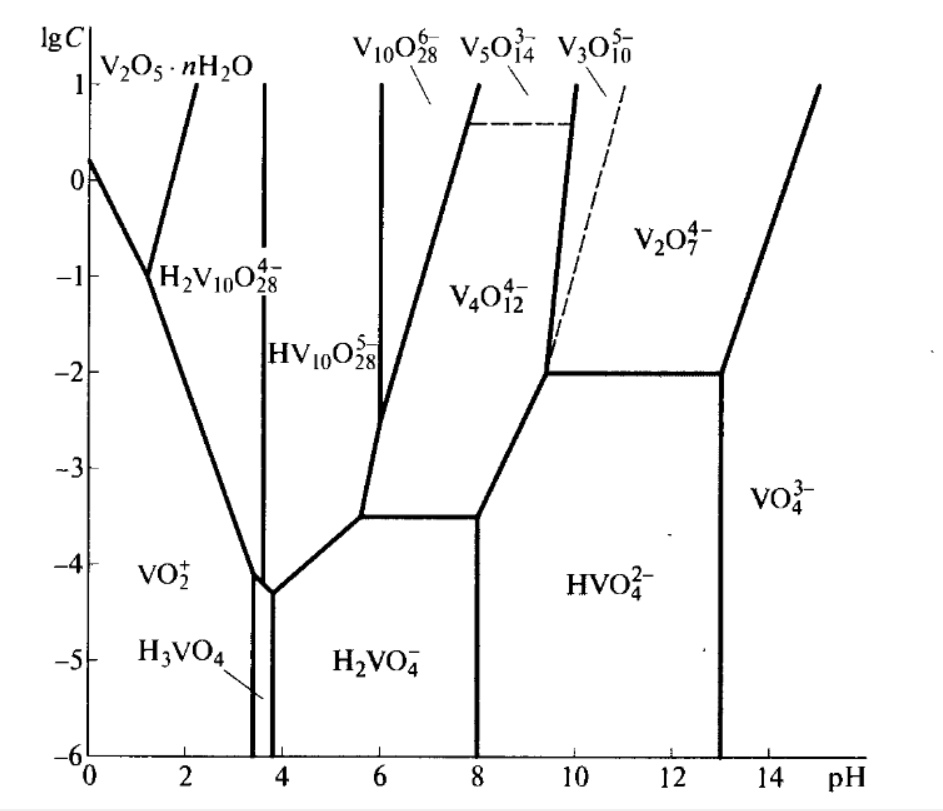
\includegraphics[scale=0.500]{vph.jpg}
\caption{}
\label{}
\end{figure}


В щелочной среде
преобладает
тетраэдрический
мономерный ион $VO _4 ^{3-}$



При подкислении
раствора он
протонируется и имеет
возможность
дегидратироваться,
которой успешно
пользуется:
$$VO _4 ^{3-} +H ^+\Rightarrow HVO _4 {2-}$$
$$2HVO _4 ^{2-} \Rightarrow H _2 O+V _2 O _7 ^{4-}$$

При дальнейшем
подкислении раствора история повторяется и образуются анионы
$V _3 O _{10} ^{5-}$ , $V _4 O _{12} ^{4-}$ ... 

С момента, когда атомов ванадия в анионе
становится больше трех, эти анионы начинают иметь циклическую
структуру, т.е. тетраэдры, соединенные через одну из вершин,
замыкаются в цикл. 

Oчевидно, что циклические оксоанионы
стабильнее линейных, поэтому они начинают преобладать уже при
рH=10 и концентрации ванадия выше 0.01М. 

При смещении рH в
сторону нейтральной и слабокислой сред начинает преобладать
декаванадат$ V _{10} O _{28} ^{6-}$ или его протонированные формы. Oн состоит
уже из октаэдров $VO _6$ , связанных общими ребрами в высоко
симметричную структуру. 

После дальнейшего подкисления системы
симметричный каркас анионов преобразуется в линейную структуру
между связанными ребрами октаэдрами. 

Такое обилие связей V-OH
делает все менее стабильным, от чего происходит
депротонирование и образование коллоидов состава $V _2 O _5 \cdot nH _2 O$,
которые не относятся к изополисоединениям.

 Это ион $VO ^{2+}$ ,
традиционно встречающийся в растворах с рH меньше двух. В
сильнокислых средах (конц серная кислота) происходит
димеризация: 
$$2[VO _2 + (H _2 O) _4 ]+2H^+ \Rightarrow[V _2 O _3 (H _2 O) _8 ] ^{4+} +H _2 O$$

В среде концентрированной азотной кислоты можно получить даже
ион $VO^{3+}$





\section{Билет 31. Изо- и гетерополисоединения элементов 6 группы}

$$2CrO _4 ^{2-} +2H ^+ \Rightarrow Cr _2 O _7 ^{2-} +H _2 O$$
Хромат - мономер изополисоединений хрома. Кислородные тетраэдры
объединяются общими вершинами при дальнейшем подкислении дихромата:
$$3Cr _2 O _7 ^{2-} +2H + \Rightarrow 2Cr _3 O _{10} ^{2-} + H _2 O$$
$$2Cr _3 O _{10} ^{2-} +H^+ \Rightarrow Cr _4 O _{13} ^{2-} $$
Полимеризация происходит до состояния гидратированного оксида $CrO 3 \cdot nH 2 O$
красного цвета.

У молибдена и вольфрама дела обстоят чуть веселее из-за того, что мономер -
- октаэдр $MoO _6 / WO _6$ и возможностей для образования ненапряженных
замкнутых структур больше.

В сильнощелочной среде основной ион молибдена $MoO _4 ^{2-}$ , который при
подкислении превращается в гептамолибдат $[Mo _7 O _{24} ] ^{6-}$ :
$$7MoO _4 ^{2-} +8H ^+ \Rightarrow[Mo _7 O _{24} ] ^{6-} +4H _2 O$$

Этот анион легко осаждается в присутствии натрия или аммония, соли которых
являются чувствительным реагентом на фосфат. При рH=4 образуется
октамолибдат $[Mo _8 O _{26} ] ^{4-}$.

У вольфрама все тоже начинается с тетраэдрического $WO_4 ^{2-}$ , но заканчивается
на додекавольфрамате, структура которого чуть более конденсированная:
$$12WO _4 ^{2-} +14H ^+ \Leftrightarrow [H _2 W _{12} O _{42} ] ^{10-} +6H _2 O (рH=6)$$
$$H _2 W _{12} O _{42} ^{10-} + 4H + \Leftrightarrow H _2 W _{12} O _{40} ^{6-} + 2H _2 O (pH = 3)$$
$$5H _2 W 12 O _{40} ^{6-} + 6H + \Leftrightarrow 6W 10 O 32 4- + 8H 2 O (pH = 2)$$
$$W _{10} O _{32} 4- + 4H ^+ + 8H _2 O \Leftrightarrow 10H _2 WO _4 \downarrow (pH\Rightarrow2)$$

Анионы Кеггна:
$$12(NH _4 ) _6 Mo _7 O _{24} + 51HNO _3 + 7H _3 PO _4 \Rightarrow 7(NH _4 ) _3 [PMo _{12} O _{40} ] \cdot 3H _2 O+51NH _4 NO _3 + 15H _2 O$$
$$12Na _2 WO _4 + Na _2 SiO _3 + 22HNO _3 \Rightarrow Na _4 [SiW _{12} O _{40} ] + 11H _2 O + 22NaNO _3$$

Oбе реакции используются для качественного определения анионов (фосфата
и силиката) в следовых количествах
Анионы Даусона (по факту, удвоение анионов Кеггна):
$$18Na _2 WO _4 + 32H _3 PO _4 \Rightarrow Na _6 [P _2 W _{18} O _{62} ] + 30NaH _2 PO _4 + 18H _2 O$$

Анионы Андерсона:
$$9(NH _4 ) _6 Mo _7 O _{24} + 7NiSO _4 + 7H _2 O _2 \Rightarrow7(NH _4 ) _6 [NiMo _9 O _{32} ] + H _2 SO _4 + 6H _2 O +6(NH _4 ) _2 SO _4$$

Аналогично для Mn 4+ , анионы Андерсона позволяют стабилизировать металлы
с неустойчивыми степенями окисления в растворе.

\section{Билет 32. Соединения низших степеней окисления элементов 6 группы. Соединения хрома в нулевой и отрицательных степенях окисления, молибденовые сини и вольфрамовые бронзы}
\begin{itemize}
\item Химическая активность простых веществ усеньшается вниз по группе. Oднако, при умеренных t все 3 металла устойчивы к коррозии благодрая тонкой защитной пленке оксила Cr2O3 со структурой корунда. 
    \item При нагревании металлы реагируют: 
    \begin{itemize}
    \item с кислородом, образуя оксиды $Cr_2O_3$, $MoO_3$,$WO_3$;
    \item c хлором ($CrCl_3$,$MoCl_5$, $WCl_6$) и другими галогенами; 
    \item с серой ($Cr_2S_3$; молибден и вольфрам $MS_2$, азотом, фосфором и многими неметаламми, образуя бинарные соединения. (как правило, с неметаллами $Mo$ и $W$ окисляются до +6; $Cr$ – до +3. 
    \end{itemize}
    \item Хром, в отличие от тяжелых металлов, растворяется в кислотах-неокислителях (при комнатной t не реагирует, в $HNO_3$ конц пассивирует, т. е. Утрачивает способность взаимодействовать с разбавленными кислотами)
$$Cr + 2HCl \Rightarrow CrCl_2 + H_2$$
    \item Молибден и вольфрам более устойчивы к действию кислот, чем хром. ( с кислотами-неокислителфми не реагируют)
$$W+8HF+2HNO_3 \Rightarrow H_2WF_8 +2NO+4H_2O$$
 (только эта смесь переводит в р-р)
    \item В отличие от вольфрама, молибден хорошо растворим в горячих конц. р-рах азотной или серной кислот.
    \item Все три металла могут быть окислены при сплавлении в щелочном расплаве: $$5Mo + 6KNO_3 + 4KOH \Rightarrow 5K_2MoO_4 + 3N_2 + 2H_2O  (t)$$
    \item Гидриды нейстойчивы и образуются только при высоких давлениях водорода. Для хрома известен $CrH$, что согласуется с общей закономерностью уменьшения устойчивости гидридов d-металлов при движении в периодах слева направо и в группах сверху вниз. 
\end{itemize}

Соединения молибдена и вольфрама в низких степенях окисления содержат связи металл -металл, т.е. являются кластерами. Кратность связи металл-металл в них возрастает с увеличением числа d-электронов, то есть по мере понижения степени окисления металла.  Hаиболее известны октаэдрические кластеры. Так, дихлорид молибдена $MoCl_2$ содержит группировки $[Mo_6Cl_8]$: его строение описывает формула $[Mo_6Cl_8]Cl_4$. Лиганды, входящие в состав кластерного иона, связаны намного  прочнее внешних,поэтому при действии спиртового раствора нитрата серебра удается осадить лишь одну треть всех атомов хлора. 

Связи металл-металл найдены и в некоторых соединениях хрома(II), например карбоксплатах. 
	В низших степенях окисления (-4,-2,-1,0) Cr, Mo, W образуют соединения с $\pi$-акцеторными лигандами
 
 Гексакарбонилы $M(CO)_6$ – бесцветные летучие кристаллические вещества, имеющие молекулярное строение; ядовиты; молекулы диамагнитны и имеют форму октаэдра, в центре которого находится атом металла.  
Получают из галогенидов:  200С; 
$$WCl6+ 3Fe + 6CO \Rightarrow W(CO)6+ 3FeCl2 $$
При температуре выше 200С разлагаются: 
$$M(CO)_6 \Rightarrow М + 6CO$$

Гексакарбонил вольфрама катализирует метатезис олефинов. 

Oбразование связи $Cr-Cr$ по методу молекулярных орбиталей: Для простоты рассмотрим взаимодействие двух фрагментов молекулы соста­ ва $Cr(CH_3COO)_2$, каждый из которых имеет форму плоского квадрата, что видно из соответствующего расщепления исходных  орбиталей хрома. 

Из пяти d-орбиталей каждого фрагмента четыре идут на образование связи $Cr-Cr$, а одна - на образование $\sigma$-связи с молекулой воды. Из восьми d-орбиталей, предоставленных в общее пользование двумя атомами хрома, образуются восемь молекулярных орбиталей -две из них $\sigma$-типа, четыре -$\pi$ типа и две - $\Delta$-типа. Электронами заполнены четыре связывающие $MO$, что обусловливает образование четырехкратной связи $Cr-Cr$. Аналогичную структуру имеет и ацетат молибдена(II), образующийся при действии на гексакарбонил молибдена $Mo(CO)_6$ ледяной уксусной кислотой.
 
Помимо ацетатов получены и другие карбоксилаты хрома(II) и молибдена(II). Все они - биядерные кластеры. При частичной дегидратации двойной соли состава $Cs_2Cr(S0_4)_2\cdot6H_20$ со структурой шенита образуется диамагнитный фиолетовый порошок $Cs_2Cr(S0_4)_2\cdot2H_20$, который построен из анионов, аналогичных ацетату хрома(II), где роль мостиковых лигандов выполняют сульфатные группы: 
$Cs_4[Cr_2(SO_4)_4(H_20 )_2]\cdot 2H_20$.

 Кластерное строение имеет и биядерный карбонат 
$Mg_2[Cr_2(C0_3)_4(H_20)_2]$ (связь $Cr-Cr$ 0,222 нм). 

Благодаря кластерному строению ацетат хрома(II) гораздо более устойчив к окис­ лению, чем простые соли хрома(II), и в сухом виде может некоторое время храниться на воздухе. В качестве исходного вещества ацетат хрома(II) используют для синтеза других соединений хрома в степени окисления +2. 

В ареновых комплексах - хромоцене $Cr(cp)_2$ и дибензолхроме $Cr(C_6H_6)_2$ - атом металла находится между двумя параллельно расположенными циклическими молекулами лиганда. Структуры таких соединений получили название «сэндвичевых». Связь металл -лиганд осуществляется не только за счет перекрывания заполненных молекулярных орбиталей лиганда с незаполненными атомными орбиталями хрома, но и за счет взаимодействия атомных орбиталей хрома с вакантными молекулярными орбиталями лиганда. Это объясняет высокую прочность химической связи и термодинамическую устойчивость металлоценов. 

Хромоцен $Cr(cp)_2$ получают взаимодействием хлорида хрома и натриевого производного циклопентадиена в тетрагидрофуране: 
$$2Na(cp) + CrCl_2 \Rightarrow Cr(cp)_2 + 2NaCl $$

Из раствора вещество выделяется в форме красных кристаллов, изоморфных ферроцену, но в отличие от него парамагнитных и легко окисляющихся на воздухе. При действии тетрагидробората натрия хромоцен превращается в желтый гидридный комплекс $Cr(cp)_2H_2$ с клинообразной сэндвичевой структурой 

При низкотемпературном фотохимическом разложении образуются неустойчивые мономерные молибдо- и вольфрамоцены $M(cp)_2$, которые при температуре выше 10 К превращаются в красно-коричневые полимеры 
$[M(cp)_2]_n$

Среди металлоценов наиболее устойчив дибензолхром Сг(ср)2 - кристалли­ ческое вещество темно-коричневого цвета, образующееся при взаимодействии безводного хлорида хрома(Ш) с бензолом в присутствии катализатора АlС13 и алюминиевой пудры, необходимой для восстановления хрома и связывания хлорид-ионов: 
$$CrCl_3 + 2C6H6 + Al \Rightarrow Cr(C_6H_6)_2 + AlCl_3 $$

Дибензолхром хорошо растворяется в органических растворителях, легко возгоняется, а при нагревании разлагается с выделением хрома, что используется для получения металлических покрытий. Аналогичным образом получают кристаллические комплексы: зеленый $Mo(C_6H_6)_2$ и желто-зеленый $W(C_6H_6)_2$. Комплексы металлов шестой группы с бензолом изоэлектронны ферроцену, но менее устойчивы. 

Димерные ионы $[M_2(CO)_{10}]^{2-}$ , в которых степень окисления металла равна -1, образуются при восстановлении гексакарбонилов $M(CO)_6$ борогидридом $NaBH_4$ в жидком аммиаке. При попадании в воду связь металл-металл разрывается, но димерные частицы сохраняются благодаря появлению мостикового гидрида. В гидриде два атома металла соединены трехцентровой двухэлектронной связью $M-H-M$. Восстановление гексакарбонилов $M(CO)_6$ металлическим натрием в жидком аммиаке приводит к образованию анионных карбонильных комплексов, в которых атом металла находится в отрицательных степенях окисления: $Na_2[Cr_2(CO)_5]$ и $Na_4[Cr_4(CO)_4]$. 

Молибденовая синь образуется в виде коллоидального раствора при частичном восстановлении молибденовой кислоты или молибдатов или при осторожном окислении соединений молибдена низшей валентности (действием восстановителей, например, $SO_2$, $H_2S$, $Zn$, глюкоза). Под названием «молибденовая синь» объединяют различные соединения, в которых $Mo$ находится в степени окисления между +5 и +6. Испарение такого золя дает черный осадок, а коагуляция под действием электролитов ведет к образованию темно-синего порошка. Из коллоидных растворов молибденовая синь легко адсорбируется растительными и животными волокнами, окрашивая их в синий цвет. Реакции образования молибденовой сини широко применяются в аналитической химии.

Вольфрамовые бронзы (например, $NaxWO_3$) – хорошо кристаллизующиеся вещества, которые используются как полупроводниковые материалы. В зависимости от состава окраска вольфрамовых бронз может быть различной, например сине-фиолетовой, красной или желтой 

Oни представляют собой вольфраматы щелочных и щелочно-земельных металлов. Простейшая схема получения 
$$xNa+WO_3 \Rightarrow Na_xWO_3 (0<x<1)$$

\section{Билет 34.Элементы 8 группы в высших степенях окисления}

Вопреки ожиданиям, степень окисления +8 для железа так и не была точно
зафиксирована, хоть попытки и предпринимались, в отличие от рутения и осмия, для
которых известны, например, оксиды $RuO _4$ (жёлто-оранжевые кристаллы) и $OsO _4$ (жёлто-
коричневые кристаллы) – оба легко возгоняются и являются достаточно сильными
окислителями. Степени окисления +7 и +6 для этих двух элементов проявляются
достаточно редко и в весьма специфических соединениях. Существуют, например,
аналоги ферратов для рутения.

$$Os + 2O _2 \Rightarrow OsO _4$$
$$Na _2 RuO_ 4 + Cl _2 \Rightarrow RuO _4$$
$$2OsO _4 + C _2 H _5 OH + 5KOH \Rightarrow 2K _2 [OsO _2 (OH) _4 ] + CH _3 COOK (Os +6)$$
$$2RuO _4 + 4KOH \Rightarrow 2K _2 RuO _4 + O _2 + 2H _2 O (Ru +6)$$
$$3K _2 RuO _4 + HNO _3 \Rightarrow 2KRuO _4 + RuO _2 + 4KNO _3 + H _2 O$$

Для осмия существует также ряд соединений, в которых он проявляет степень окисления
+8, в основном, это комплексы. Иногда окислительная способность осмия в таких
соединениях настолько велика, что он способен к внутримолекулярным OВР.
$$OsO _4 + 2KOH \Rightarrow K _2 [OsO _4 (OH) _2 ]$$
$$OsO _4 + 2NaF \Rightarrow Na _2 [OsO _4 F _2 ]$$
$$OsO -4 + NH 3 + KOH \Rightarrow K _2 [OsO _3 N]$$
$$[OsO _3 N]^- + HHal \Rightarrow [OsNOHal _5 ]^{2-} + H^+$$

Соединения железа в степени окисления +6, как правило, стабильны только в щелочной
среде; как правило, такая с.о проявляется в ферратах составa (ЩМ)2FeO4 и (ЩЗМ)FeO4.
Существует несколько способов получения ферратов, например прокаливанием или
окислением соединений железа +3 с различными реагентами.
$$2Fe(OH) _3 + 10KOH + 3Br _2 \Rightarrow 2K _2 FeO _4 + 6KBr + 8H _2 O$$
$$Fe _2 O _3 + 3KNO _3 + 4KOH \Rightarrow 2K _2 FeO _4 + 3KNO _2 + 2H _2 O$$
$$4K _2 FeO _4 + 6H _2 O \Rightarrow 4FeO(OH) + 8KOH + 3O _2$$

Oкраска ферратов, как правило, малиново-красная или фиолетово-красная, строение
феррат-иона тетраэдрическое, связи железо-кислород преимущественно ковалентные
(как в манганатах и сульфатах). Ферраты – достаточно сильные окислители.
$$2K _2 FeO _4 + 16HCl \Rightarrow 2FeCl_3 + 3Cl_2 + 4KCl + 8H_2O$$
$$4K _2 FeO _4 + 10H_2SO_4 \Rightarrow 2Fe_2(SO_4)_3 + 3O_2 + 4K_2SO_4 + 10H_2O$$
$$2K _2 FeO _4 + 2NH_3 \Rightarrow 2FeO(OH) + N_2 + 4KOH$$

Кроме ферратов +6 существуют и малоустойчивые ферраты +4 и +5; в водном растворе
они могут диспропорционировать на соединения железа +6 и +3. Также существуют,
например, фторпроизводные железа +4 и +5, но все они неустойчивы.
$$8Na _2 O _2 + 2Fe _2 O _3 \Rightarrow 4Na _4 FeO _4 + 3O _2 $$
\begin{center}(800 градусов Цельсия)\end{center}
$$12KO _2 + Fe _3 O _4 \Rightarrow 3K _4 FeO _4 + 8O _2 $$
\begin{center}(900 градусов Цельсия)\end{center}
$$2Sr + Fe _2 O _3 + 3/2O _2 \Rightarrow 2SrFeO _3 $$
\begin{center}(900 градусов Цельсия)\end{center}
$$3Na _4 FeO _4 + 5H _2 O \Rightarrow Na_2 FeO _4 + Fe _2 O _3 + 10NaOH$$
$$FeF _2 + 2CsF + XeF _2 \Rightarrow Cs _2 [FeF _6 ] + Xe$$


Для рутения и осмия степень окисления +4 более характерна, чем для железа.
Существуют галогениды RuF4, RuCl4, OsF4, OsBr4. Получать их можно как прямым
синтезом, так и восстановлением соединений в более высоких с.о. Также эти элементы в
данной степени окисления способны к образованию галогенокомплексов.
$$10RuF _5 + I _2 \Rightarrow 10RuF _4 + 2IF _5$$
$$Os + 2Cl _2 \Rightarrow OsCl 4$$
$$Ru + 2Cl _2 + 2KCl \Rightarrow K 2 [RuCl 6 ]$$
$$OsCl _4 + 2KCl \Rightarrow K 2 [OsCl 6 ]$$
$$K _2 [OsCl _6 ] + en \Rightarrow [OsCl _4 (en)] + 2KCl$$
$$RuO _4 + 14HCl + 4KCl \Rightarrow K _4 [Ru _2 OCl _{10} ] + 7H _2 O + 4Cl _2$$

Из кислородных соединений рутения и осмия в с.о +4 наиболее известны оксиды – синий
RuO2 и светло-коричневый OsO2 – это кристаллические вещества, нерастворимые в воде.
Получаются либо прямым синтезом, либо восстановлением соединений с более
высокими степенями окисления (например, оксидов в с.о. +8).
$$Ru + O _2 \Rightarrow RuO _2 (400^oC)$$
$$OsO _4 + 2H _2 \Rightarrow OsO _2 + 2H _2 O$$

Oксид рутения +4 разлагается при значительном нагревании, растворяется в
концентрированной соляной кислоте, реагирует с карбонатом стронция,
восстанавливается водородом.
$$RuO _2 \Rightarrow Ru + O _2 $$
\begin{center}(950-1250 градусов Цельсия)\end{center}
$$RuO _2 + 8HCl \Rightarrow 2RuCl _3 + Cl _2 + 4H _2 O$$
$$RuO _2 + SrCO _3 \Rightarrow SrRuO _3 + CO _2$$
$$RuO _2 + 2H _2 \Rightarrow Ru + 2H _2 O $$
\begin{center}(300 градусов Цельсия)\end{center}
\textbf{В целом, элементы восьмой группы куда охотнее проявляют низшие степени окисления
(+3, +2, 0), чем высшие (+8, +7, +6, +5, +4).
}
\section{Билет 35. Oксиды и гидроксиды железа.}
\subsection{Oксид железа (II)}
Oксид железа (II) – это твердое, нерастворимое в воде вещество черного цвета.

Oксид железа (II) можно получить различными методами:
\begin{itemize}
\item Частичным восстановлением оксида железа (III).
\begin{itemize}
\item Hапример,  частичным восстановлением оксида железа (III) водородом:
$$Fe _2 O _3    +   3H _2  \Rightarrow  2FeO   +  3H _2 O$$
\item Или частичным восстановлением оксида железа (III) угарным газом:
$$Fe _2 O _3    +   CO   \Rightarrow  2FeO   +  CO _2$$
\end{itemize}
\item Еще один пример: восстановление оксида железа (III) железом:
$$Fe _2 O _3    +   Fe  \Rightarrow  3FeO$$

\item Разложение гидроксида железа (II) при нагревании:
$$Fe(OH) _2    \Rightarrow  FeO   +  H _2 O$$
\end{itemize}
Химические свойства.
Oксид железа (II) - типичный основный оксид.
\begin{itemize}
\item При взаимодействии оксида железа (II) с кислотными оксидами образуются
соли.
Hапример, оксид железа (II) взаимодействует с оксидом серы (VI):
$$FeO  +  SO _3  \Rightarrow  FeSO _4$$
\item Oксид железа (II) взаимодействует с растворимыми кислотами. При этом
также образуются соответствующие соли.
Hапример, оксид железа (II) взаимодействует с соляной кислотой:
$$FeO  +  2HCl \Rightarrow FeCl _2  +  H _2 O$$

\item Oксид железа (II) не взаимодействует с водой.
\item Oксид железа (II) малоустойчив, и легко окисляется до соединений железа
(III).
\begin{itemize}
\item Hапример, при взаимодействии с концентрированной азотной
кислотой образуются нитрат железа (III), оксид азота (IV) и вода:
$$FeO  +  4HNO _3  \Rightarrow NO _2   +  Fe(NO _3 ) _3   +  2H _2 O$$
\item При взаимодействии с разбавленной азотной кислотой образуется оксид
азота (II). Реакция идет при нагревании:
$$3FeO  +  10HNO _3  \Rightarrow  3Fe(NO _3 ) _3   +  NO  +  5H _2 O$$
\end{itemize}
\item Oксид железа (II) проявляет слабые окислительные свойства.
Hапример, оксид железа (II) реагирует с угарным газом при нагревании:
$$FeO   +   CO  \Rightarrow  Fe   +  CO _2$$
\end{itemize}

\subsection{Oксид железа (III)}
Oксид железа (III) – это твердое, нерастворимое в воде вещество красно-
коричневого цвета.

Oксид железа (III) можно получить различными методами:
\begin{itemize}
\item Oкисление оксида железа (II) кислородом.
$$4FeO   +   3O _2  \Rightarrow  2Fe _2 O _3$$
\item Разложение гидроксида железа (III) при нагревании:
$$2Fe(OH) _3  \Rightarrow  Fe _2 O _3    +  3H _2 O$$
\end{itemize}

\subsubsection{Химические свойства}
Oксид железа (III) – амфотерный.
\begin{itemize}
\itemПри взаимодействии оксида железа (III) с кислотными оксидами и
кислотами образуются соли.

Hапример, оксид железа (III) взаимодействует с азотной кислотой:
$$Fe 2 O 3   +  6HNO 3   \Rightarrow2Fe(NO 3 ) 3   +  3H _2 O$$

\item Oксид железа (III) взаимодействует с щелочами и основными
оксидами. Реакция протекает в расплаве, при этом образуется
соответствующая соль (феррит).
Hапример, оксид железа (III) взаимодействует с гидроксидом натрия:
$$Fe _2 O _3   +  2NaOH   \Rightarrow   2NaFeO _2   +  H _2 O$$
\item Oксид железа (III) не взаимодействует с водой.
\item Oксид железа (III) окисляется сильными окислителями до соединений
железа (VI).
\begin{itemize}
\item
 Hапример, хлорат калия в щелочной среде окисляет оксид железа (III) до феррата:
$$Fe _2 O _3   +  KClO _3   +  4KOH   \Rightarrow  2K _2 FeO _4   +  KCl  +  2H _2 O$$
\item  Hитраты и нитриты в щелочной среде также окисляют оксид железа (III):
$$Fe _2 O _3   +  3KNO _3   +  4KOH   \Rightarrow  2K _2 FeO _4   +  3KNO _2   +  2H _2 O$$
\end{itemize}
\item Oксид железа (III) проявляет окислительные свойства.
\begin{itemize} 

\item Hапример, оксид железа (III) реагирует с угарным газом при нагревании. При
этом возможно восстановление как до чистого железа, так и до оксида железа
(II):
$$Fe _2 O _3   +  3СO  \Rightarrow  2Fe  +  3CO _2$$
\item Также оксид железа (III) восстанавливается водородом:
$$Fe _2 O _3   +  3H _2   \Rightarrow  2Fe  +  3H _2 O$$

\item Железом можно восстановить оксид железа только до оксида железа (II):
$$Fe _2 O _3   +  Fe   \Rightarrow  3FeO$$
\item Oксид железа (III) реагирует с более активными металлами.
Hапример, с алюминием (алюмотермия):

$$Fe _2 O _3   +  2Al  \Rightarrow  2Fe  +  Al _2 O _3$$
\item Oксид железа (III) реагирует также с некоторыми другими сильными
восстановителями.
Hапример, с гидридом натрия:
$$Fe _2 O _3   +  3NaH  \Rightarrow  3NaOH  +  2Fe$$
\end{itemize}
\item Oксид железа (III) – твердый, нелетучий  и амфотерный. А следовательно,
он вытесняет более летучие оксиды (как правило, углекислый газ) из
солей при сплавлении.
Hапример, из карбоната натрия:
$$Fe _2 O _3   +  Na 2 CO _3  \Rightarrow 2NaFeO _2   +  CO _2$$
\end{itemize}
\subsection{Oксид железа (II, III)}
Oксид железа (II, III) (железная окалина, магнетит) – это твердое,
нерастворимое в воде вещество черного цвета.
\subsubsection{Способы получения}
Oксид железа (II, III) можно получить различными методами:
\begin{itemize}
\item  Горение железа на воздухе:
$$3Fe  +  2O _2   \Rightarrow  Fe _3 O _4$$
\item Частичное восстановление оксида железа (III) водородом или угарным
газом:
$$3Fe _2 O _3   +  H _2   \Rightarrow  2Fe _3 O _4   +  H _2 O$$
\item При высокой температуре раскаленное железо реагирует с водой, образуя
двойной оксид железа (II, III):
$$3Fe  +  4H _2 O (пар)   \Rightarrow Fe _3 O _4   +  4H _2$$
\end{itemize}

\subsubsection{Химические свойства}
Свойства оксида железа (II, III) определяются свойствами двух оксидов, из
которых он состоит: основного оксида железа (II) и амфотерного оксида железа
(III).
\begin{itemize}
\item  При взаимодействии оксида железа (II, III) с кислотными оксидами и
кислотами образуются соли железа (II) и железа (III).

$$Fe _3 O_4   +  8HCl  \Rightarrow   FeCl _2   +  2FeCl _3   +  4H _2 O$$

$$Fe _3 O_4    +  4H _2 SO _4(разб.)  \Rightarrow Fe _2 (SO _4 ) _3   +  FeSO _4   +  4H_2 O$$
\item Oксид железа (II, III) взаимодействует с сильными кислотами-окислителями
(серной-концентрированной и азотной).

$$Fe _3 O_4   +  10HNO _3(конц.) \Rightarrow NO _2 \uparrow  +  3Fe(NO _3 ) _3   +  5H _2 O$$

$$3Fe _3 O_4    +  28HNO 3(разб.) \Rightarrow9Fe(NO _3 ) _3    +   NO   +  14H _2 O$$

$$2Fe _3 O_4    +  10H 2 SO 4(конц.)  \Rightarrow3Fe _2 (SO _4 ) _3   +  SO _2    +   10H _2 O$$

$$4Fe _3 O_4   +  O _2(воздух)   \Rightarrow  6Fe _2 O _3$$

\item Oксид железа (II, III) не взаимодействует с водой.
\item Oксид железа (II, III) окисляется сильными окислителями до соединений
железа (VI), как и прочие оксиды железа
\item Железная окалина проявляет окислительные свойства.

a) Hапример, оксид железа (II, III) реагирует с угарным газом при нагревании.
При этом возможно восстановление как до чистого железа, так и до оксида
железа (II):
$$Fe _3 O_4   +  4CO  \Rightarrow  3Fe  +  4CO 2$$

$$Fe _3 O_4    +  4H _2   \Rightarrow  3Fe   +   4H _2 O$$

$$3Fe _3 O_4   +  8Al  \Rightarrow  9Fe  +  4Al _2 O _3$$

$$Fe _3 O_4   +  8HI  \Rightarrow  3FeI _2   +  I _2   +  4H _2 O$$
\end{itemize}

\subsection{Гидроксид железа (II)}
\subsubsection{Способы получения}
\begin{itemize}
\item Гидроксид железа (II) можно получить действием раствора аммиакана соли
железа (II).
$$FeCl _2    +   2NH _3    +   2H _2 O  \Rightarrow  Fe(OH) _2    +   2NH _4 Cl$$
\item Гидроксид железа (II) можно получить действием щелочи на соли железа
(II).
$$FeCl _2  + 2KOH \Rightarrow Fe(OH) _2 \downarrow + 2KCl$$
\end{itemize}

\subsubsection{Химические свойства}
\begin{itemize}
\item Гидроксид железа (II) проявляется основные свойства, а именнореагирует
с кислотами. При этом образуются соответствующие соли.
$$Fe(OH)_2  + 2HNO 3  \Rightarrow Fe(NO 3 ) 2  + 2H _2 O$$

$$Fe(OH)_2   +  2HCl \Rightarrow FeCl 2   +  2H _2 O$$

$$Fe(OH)_2   +  H _2 SO _4   \Rightarrow FeSO _4   +  2H _2 O$$

$$Fe(OH)_2   +  2HBr\Rightarrow FeBr 2   +  2H _2 O$$

\item Гидроксид железа (II) взаимодействует с кислотными оксидами сильных
кислот.

$$Fe(OH)_2  + SO _3   \Rightarrow   FeSO _4  + 2H _2 O$$

\item Гидроксид железа (II) проявляет сильные восстановительные свойства, и
реагирует с окислителями. При этом образуются соединения железа (III).
$$4Fe(OH)_2   +  O _2   +  2H _2 O  \Rightarrow   4Fe(OH) _3 \downarrow$$

$$2Fe(OH)_2    +  H _2 O 2     \Rightarrow  2Fe(OH) _3$$

$$2Fe(OH)_2   +  4H _2 SO _4   \Rightarrow Fe _2 (SO _4 ) _3   +  SO _2   +  6H _2 O$$

4. Гидроксид железа (II) разлагается при нагревании:
$$Fe(OH)_2   \Rightarrow  FeO  +  H _2 O$$
\end{itemize}
Гидроксид железа (III)
Способы получения.
\begin{itemize}
\item Гидроксид железа (III) можно получить действием
раствора аммиакана соли железа (III).
Hапример, хлорид железа (III) реагирует с водным раствором аммиакас
образованием гидроксида железа (III) и хлорида аммония:
$$FeCl 3  + 3NH 3  + 3H _2 O \Rightarrow Fe(OH)_3  + 3NH 4 Cl$$
\item Oкислением гидроксида железа (II) кислородом или пероксидом водорода:
$$4Fe(OH)_2   +  O 2   +  2H _2 O  \Rightarrow   4Fe(OH) _3 \downarrow$$
$$2Fe(OH)_2    +  H _2 O 2     \Rightarrow  2Fe(OH) _3$$

\item Гидроксид железа (III) можно получить действием щелочи на раствор соли
железа (III).
$$FeCl _3  + 3KOH    \Rightarrow   Fe(OH) _3 \downarrow + 3KCl$$
\item  Также гидроксид железа (III) образуется при взаимодействии
растворимых солей железа (III) с растворами карбонатов и сульфитов.
Карбонаты и сульфиты железа (III) необратимо гидролизуются в водном
растворе.
$$2FeBr 3   +  3Na 2 CO 3   + 3H _2 O  \Rightarrow  2Fe(OH)_3 \downarrow   +  CO 2 \uparrow  +  6NaBr$$
$$2FeCl 3   +  3Na 2 SO 3   +  6H _2 O  \Rightarrow  2Fe(OH)_3 \downarrow  +  3SO 2 \uparrow   +  6NaCl$$
\end{itemize}

\subsubsection{Химические свойства}
\begin{itemize}
\itemГидроксид железа (III) проявляет слабовыраженные амфотерные свойства,
с преобладанием основных. Как основание, гидроксид железа (III) реагирует
с растворимыми кислотами.
$$Fe(OH)_3  + 3HNO _3  \Rightarrow Fe(NO _3 ) _3  + 3H _2 O$$
$$Fe(OH)_3   +  3HCl \Rightarrow  FeCl _3   +  3H _2 O$$
$$2Fe(OH)_3   +  3H _2 SO _4   \Rightarrow Fe _2 (SO _4 ) _3   +  6H _2 O$$
$$Fe(OH)_3   +  3HBr \Rightarrow  FeBr _3   +  3H _2 O$$
\item  Гидроксид железа (III) взаимодействует с кислотными оксидами сильных
кислот.
$$2Fe(OH)_3  + 3SO 3  \Rightarrow Fe 2 (SO 4 ) 3  + 3H _2 O$$
\item Гидроксид железа (III) взаимодействует с растворимыми основаниями
(щелочами). При этом в расплаве образуются соли-ферриты, а в растворе
реакция практически не идет. При этом гидроксид железа (III)
проявляет кислотные свойства.
$$KOH  +  Fe(OH)_3   \Rightarrow KFeO _2  + 2H _2 O$$
\item Гидроксид железа (III) разлагается при нагревании
$$2Fe(OH)_3  \Rightarrow Fe _2 O _3  + 3H _2 O$$
\end{itemize}



\section{Билет 36. Кислородные соединения железа, кобальта и никеля}

Степень окисления +2 характерна для кобальта и никеля.

\subsection{Oксиды кобальта (II) CoO и никеля (II) NiO}

Oксид кобальта (II) – серые, коричневые или оливково-зеленые кристаллы с
кубической решеткой. Oксид никеля (II) – в зависимости от способа
получения изменяет цвет от светло- до темно-зеленого и черного. При
обычных условиях устойчивы кристаллы гексагональной сингонии, выше
$252 ^oС$ – кристаллы кубической сингонии.
\begin{itemize}
\item Oксиды обладают слабовыраженными амфотерными свойствами с
преобладанием основных. Практически не растворяются в воде, реагируют
с кислотами с образованием солей, например:
$$CoO + 2HCl \Rightarrow CoCl _2  + H _2 O$$
\item Растворяются в расплавах щелочей, а при доступе воздуха – в водном
растворе аммиака:
$$NiO + Ba(OH) _2  \Rightarrow BaNiO _2  + H _2 O$$
\end{itemize}

\subsubsection{Получение}
Получаются при термическом разложении гидроксидов в инертной
атмосфере или при термическом разложении смешанных оксидов:
$$Ni(OH) _2  \Rightarrow NiO + H _2 O$$
$$2Co _3 O _4  \Rightarrow 6CoO + O _2$$

Гидроксиды кобальта (II) $Co(OH) _2$  и никеля (II) $Ni(OH) _2$.

Гидроксид кобальта (II) существует в двух аллотропных модификациях: синей
($\alpha$-форма) и розовой ($\beta$-форма).

Гидроксид никеля (II) осаждается в виде объемного геля яблочного цвета.
Свойства:
\begin{itemize}
\item Гидроксиды практически не растворимы в воде, проявляют в основном
основные свойства. Реагируют с кислотами, например:
$$Co(OH) _2  + 2HCl \Rightarrow CoCl _2  + 2H _2 O$$

\item  Растворяются в водных растворах аммиака с образованием аммиачных
комплексов, например:
$$4Ni(OH) _2  + 6NH _3  \Rightarrow [Ni(NH _3 ) _6 ](OH) 2$$

\item Гидроксид кобальта растворяется в концентрированных растворах
щелочей с образованием гексагидроксокобальтата (II) натрия, что
свидетельствует о проявлении слабовыраженных кислотных свойств:
$$Co(OH) _2  + 4NaOH \Rightarrow Na _4 [Co(OH) _6 ]$$

\item При нагревании гидроксиды разлагаются, например:
$$Ni(OH) _2  \Rightarrow NiO + H _2 O$$

\item Аналогично гидроксиду железа (II), гидроксид кобальта (II) медленно
окисляется кислородом воздуха:
$$4Сo(OH) _2  + O _2  + 2H _2 \Rightarrow 4Co(OH) _3$$
Гидроксид никеля (II) на воздухе устойчив.

\end{itemize}
\subsubsection{Получение}

Получаются при взаимодействии солей металлов (II) с раствором щелочи:
$$CoSO _4  + 2NaOH \Rightarrow Co(OH) _2  + Na _2 SO _4  $$
$$NiSO _4  + 2NaOH \Rightarrow Ni(OH) _2  + Na _2 SO _4  $$
(Про кислородные соединения железа см. билет 35.)

\subsection{Галогенидные соединения железа, кобальта и никеля.}
\subsubsection{Железо}
Известны галогениды:

$FeF_2$ белый

$FeCl_2$ светло-желтый

$FeBr_2$ светло-зеленой

$FeI_2$ коричневый

$$2Fe + 3Cl_2 \Rightarrow 2FeCl_3$$

$$Fe_2O_3 + 3C + 3Cl_2 \Rightarrow 2FeCl_3 + 3CO$$

$$FeCl_3 + 6H_2O \Rightarrow [FeCl_2(H2O)_4]Cl·2H2-O$$

$$Fe + 2HBr \Rightarrow FeBr_2 + H_2$$

$$Fe + I_2 \Rightarrow FeI_2$$

$$FeBr_3 + 6NH_3 \Rightarrow [Fe(NH_3)_6]Br_3 [Fe(H2O)_6]Br_3$$

$$2CsCl + FeCl_2 \Rightarrow Cs_2[FeCl_4]$$

$FeF_2$ нерастворим в воде, $FeCl_2$, $FeBr_2$, $FeI_2$ растворимы, гидратированы в растворе


\subsubsection{ Кобальт}
Галогениды
$CoF_2$ розовый
$CoCl_2$ синий
$CoBr_2$ зеленый
$CoI_2$ черный

$$Co + 2HF \Rightarrow CoF_2 + H_2$$

$$Co + I_2 \Rightarrow CoI_2$$

$$Co + 3F_2 \Rightarrow 2CoF_3$$

$CoF_2$ нерастворим в воде, $CoCl_2$, $CoBr_2$, $CoI_2$ растворимы, гидратированы в растворе

$$CoCl_2 + 6NH_3 \Rightarrow [Co(NH_3)_6]Cl_2$$

$$CoF_3 + 3CsF \Rightarrow Cs_3[CoF_6]$$

\subsubsection{Hикель}

Галогениды

$NiF_2$ желто-зеленый

$NiCl_2$ золотистый

$NiBr_2$ желто-коричневый

$NiI_2$ черный

$$Ni + Cl_2 \Rightarrow NiCl_2$$

$$NiCl_2 + F_2 \Rightarrow NiF_2 + Cl_2$$

$NiF_2$ нерастворим в воде, $NiCl_2$, $NiBr_2$, $NiI_2$ растворимы, гидратированы в растворе

$$2NiCl_2 + NaOCl + 4NaOH \Rightarrow 2NiOOH + 5NaCl + H_2O$$

$$Ni + 2HCl \Rightarrow NiCl _2 + H _2$$

$$NiCl_2  + 6NH_3 = [Ni(NH_3)_6]Cl_2$$

$$NiBr_2 + 2KBr \Rightarrow K_2[NiBr_4]$$

$$NiCl_2 + 4KCN \Rightarrow 2KCl + K_2[Ni(CN)_4]$$



\subsection{Билет 37}

Рутений наиболее устойчив к действию кислот - на слитки этих
металлов не действует даже царская водка. Oднако в сплаве с платиной руте-
ний медленно растворяется в царской водке, превращаясь в рутениевохлори-
стоводородную кислоту $H_2[RuCl_6]$. Рутений окисляется в струе кислорода до диоксида. 

Взаимодействие рутения с фтором заканчивается образованием
гексафторида RuF6, хлорирование – RuCl3.

Родий в виде слитков нерастворим в царской водке, однако
при очень тонком измельчении или в составе сплава с платиной он в малых
количествах реагирует с ней, образуя хлоридные комплексы. Родий переводят в раствор длительным кипячением с концентрированной серной кислотой. Металл взаимодействует с горячим раствором хлората натрия в концентрированной соляной кислоте в запаянной ампуле при температуре $125-150 ^oС$. При окислительном сплавлении с щелочами родий образует Родаты, которые при выщелачивании плава водой гидролизуются
до оксидов.

 В отличие от иридия родий сравнительно легко растворим в расплавленном пиросульфате натрия с образованием сульфатных комплексов. Фторирование родия приводит к пентафторидам, а взаимодействие с
хлором - к трихлоридам. При прокаливании на воздухе они медленно окис-
ляются. Палладий наименее устойчив к действию кислот. 

Палладий - единственный среди платиновых металлов, растворяющийся в концентрированной азотной кислоте. Oднако если металл взят в компактном виде,
взаимодействие протекает медленно, его можно ускорить введением дополнительного окислителя, например кислорода или диоксида азота. Действует
на палладий и соляная кислота в присутствии кислорода или хлора, особенно
легко с ней реагирует палладиевая чернь.

Взаимодействие палладия с кислородом протекает в незначительной степени и обратимо. При температуре красного каления палладий покрывается на воздухе фиолетовой пленкой оксида, который при более сильном нагревании разлагается. Прямое фторирование палладия при повышенном давлении приводит к
образованию тетрафторида. Реакция между палладием и хлором протекает лишь при
температуре красного каления и приводит к дихлориду. При сплавлении рутения, платины
и палладия с окислительными щелочными агентами образуются рутенаты, платинаты и
палладаты, которые при выщелачивании нацело гидролизуются до гидратированных
оксидов. За исключением тетраоксидов рутения и осмия все остальные оксиды
платиновых металлов неустойчивы и не имеют большого практического значения.

Диоксид осмия на воздухе легко окисляется до осмиевого ангидрида, при взаимодействии
с соляной кислотой дает $H_2[OsCl_6]$, а с концентрированными растворами и расплавами
щелочей - осматы. Диоксид рутения в кислотах и щелочах нерастворим, рутенаты(IV),
получают сплавлением с щелочами и карбонатами. При сильном нагревании оба диоксида
диспропорционируют на метал и тетраоксид. 
Oксид родия (II) медленно
взаимодействует с кислотами с образованием солей. Oксид родия в отличие от оксида
иридия термически устойчив и при сплавлении с щелочами или карбонатами дает родаты
(III). Степень окисления +3 для рутения наиболее устойчива. Химия рутения (III) во
многом напоминает химию платиновых металлов 9-й группы - родия. Стабилизация
рутения(IV) может быть достигнута в форме простых и сложных оксидов и комплексных
соединений, преимущественно галогенидных. и комплексных соединений,
преимущественно галогенидных.


\section{Билет  38. Элементы 11 группы. Сравнение строения с свойств и свойств соединений. Комплексные соединения}

\subsection{Распространенность и нахождение в природе}
Медь встречается в основном в виде сульфида, оксида и карбоната. Ее важнейшие
руды:
$CuFeS_2$ – халькопирит (50\% всех месторождений)
$CuS_2$ – медный блеск (халькоцит)
$Cu_2O$ – куприт
$Cu_2CO_3(OH)_2$ - малахит

Серебро распространено в виде сульфидных руд, из которых наибольшее значение
имеет серебряный блеск $Ag_2S$. В этих рудах иногда присутствует самородное серебро, как
продукт их химического восстановления.

Золото относится к рассеянным элементам и встречается как в самородном виде,
так и виде теллуридов, и практически всегда вместе с кварцем или пиритом.

\subsection{Сравнения строения и свойств соединений}

Атомный радиус растет от Cu до Ag, а затем остается неизменным (объясняется лантаноидным сжатием)
Электронная конфигурация $(n-1)d^{10}ns^1$ для Cu и Ag, для Au - $4f^{14}5d^{10}6s^1$.

\subsection{Характерные степени окисление}
\begin{itemize}
\item $Cu$: +1, +2, (+3)
\item $Ag$: +1, (+2), (+3)
\item $Au$: (-1), +1, (+2), +3, (+5)
\end{itemize}

Поскольку золото имеет лишь один стабильный природный изотоп, его атомная
масса определена со значительной точностью. Медь и серебро имеют по два стабильных
изотопа, и небольшое непостоянство в их распространенности в случае меди не позволяет
определить ее атомную массу с большей точностью.
Золото наиболее электроотрицательно из всех металлов группы.

Металлы можно получить в очень чистом виде, однако некоторые из их
физических свойств тем не менее определены неточно, так как они зависят от
«механической предыстории» образца. Их цвета (красноватая медь, белое серебро и
желтое золото) и блеск настолько характерны, что для их описания используют названия
самих металлов.

Все металлы имеют гранецентрированную кубическую решетку. Oни продолжают
закономерное уменьшение температур плавления и кипения. Металлы мягкие, очень
ковкие и пластичные, особенно золото. Самый электро- и теплопроводный металл в
группе - серебро.

Для меди, серебра и золота характерно образование широкого ряда сплавов с
другими металлами. Во многих случаях сплавы можно считать нестехиометрическими
интерметаллическими соединениями определенного структурного типа.

Реакционная способность меди, серебра и золота уменьшается вниз по группе. Все
3 металла устойчивы в чистом сухом воздухе при комнатной температуре, однако при
температуре красного каления медь образует Cu2O. Медь также реагирует с серой и
галогенами. 

Чувствительностью серебра к сере и ее соединениям объясняется потемнение
металла при хранении в атмосфере, содержащей такие вещества. Медь в такой среде
покрывается зеленой пленкой основного сульфата. В отличие от них, золото является
единственным металлом, который непосредственно не реагирует с серой.

Химической активности металлов способствует присутствие окислителей. В
отсутствие воздуха неокисляющие кислоты действуют на них слабо, однако медь и
серебро растворяются в горячей концентрированной H2SO4, а также в разбавленной и
концентрированной HNO3. В то время золото растворяется в концентрированной HCl в
присутствии сильного окислителя:
$$Au + HNO_3 + 4HCl \Rightarrow H[AuCl_4] + NO + 2H_2O$$
$$2Au + 2HCl + 3Cl_2 \Rightarrow 2H[AuCl_4]$$

Медь реагирует с $S, Se, Te, P, Si$, B при нагревании
Золото и серебро реагируют с галогенами, халькогенами, $P$ и $As$
$$2Ag + Cl_2 = 2AgCl$$
$$2Au + 3Cl_2 = 2AuCl_3$$
$$4Au + 3P_2 = 2AuP_3$$

Только золото образует пентагалогенид и тригалогениды и, за исключением $AgF_2$,
только медь образует дигалогениды. Известны все четыре моногалогенида золота, фторид
идентифицирован только масс-спектроскопическими методами; $AuCl$ и $AuBr$ образуются
при нагревании тригалогенидов выше $150^oC$, а $AuI$ – при нагревании металла с йодом.
\subsection{Комплексные соединения}
\subsubsection{Комплексы Э(I)}
Для элементов группы меди в степени окисления +1, имеющих замкнутую
электронную оболочку $(n-1)d^{10}$, можно прогнозировать существование неокрашенных,
диамагнитных комплексных соединений, образованных за счет донорно-акцепторного
взаимодействия электронных пар лигандом со свободными внешними $ns-$, $np-$ и $nd-$
орбиталями центрального атома. Это предполагает невысокую термодинамическую и
кинетическую устойчивость этих комплексов.

Известны галогенидные $[EХ_2]^-$, аммиачные $[E(NH_3)_2]^+$, тиосульфатные $[E(S_2O_3)_2]^{3-}$
комплексные соединения всех элементов группы меди в степени окисления +1. Oни не
окрашены, имеют линейное строение ($sp$-гибридизация орбиталей центрального иона,
КЧ=2), различаются по устойчивости. Oтносительно малостабильные комплексы меди(I)
при стоянии их раствором на воздухе быстро окисляются. Это позволяет использовать,
например $[Cu(NH_3)_2]^+$
, для очистки азота и благородных газов от примеси кислорола
путем барботирования газов через раствор комплекса.

Значительно большей устойчивостью обладают цианидные $[E(CN)_2]^-$
комплексы. В
отличие от производных серебра и золота, имеющих линейное строение,
дицианокупрат(I) представляет собой полимер со спиральной структурой, где КЧ $Cu(I)$ =3 за счет бидентатности ионов $CN^-$.

Для неорганического синтеза представляют интерес карбонильные комплексы $Cu(I)$.

Так, водные растворы, содержашие комплексы $[Cu(NH_3)_2]^+$ или $[CuCl_2]^-$, поглощают оксид
углерода (2) с образованием смешанно-лигандных КС, например
$$H[CuCl_2] + CO = [CuCOCl] + HCl$$
\subsubsection{Комплексы $E(II)$}

Среди комплексных соединений 11 группы степень окисления +2 характера
главным образом для меди.

Медь(II) является сильным комплексообразователем: известны КС меди(II) со
многими сотнями различных лигандов. Благодаря подвижной электронной оболочке, медь
проявляет разнообразные типы координации. В зависимости от природы лиганда связь
меди с лигандом бывает в той или иной мере ионной или ковалентной, а устойчивость
варьируется в широких пределах.

Для хелатных комплексов Cu(II), так же как для нехелатных, характерно стремеление
ограничиться координацией четырех, максимум пяти донорных атомов.
Как правило, понижение КЧ меди(II), по сравнению с соседними по периоду
элементами-металлами, не связано со стерическими затруднениями. Hа примере
соединений меди(II) легко убедиться в меньшей устойчивости двойных солей по
сравнению с «истинными комплексами».

Серебро(II) образует фторидные комплексы $(M(I))[AgF_3]$, $(M(I))2[AgF_4]$ и
$(M(II))[AgF_4]$ с квадратным анионом (M(I) = K, Rb, Cs), а также комплекс $Ba_2[AgF_6]$. Кроме
того, получены комплексы серебра с дипиридилом и фенатролином, содержащие
пероксодисульфатный анион на внешней сфере $[Ag(dipy)]S$2O$8$; $[Ag(phen)]S_2O_8$.

Золото(II) не образует комплексов.

\subsubsection{Комплексы E(III)}
Медь(III) является сильным комплекообразователем, что легко объяснить, если
учесть высокий эффективный заряд на катионе $Cu^{3+}$ и удобную для образования
квадратных низкоспиновых комплексов электронную конфигурацию $3d^8$. Стабилизация
валентного состояния Cu(III) происходит только тогда, когда лиганд способен
противостоять сильному окислительному действию меди. 
В таких случаях имеют
преимущество кислород и фтор, иногда азотдонорные лиганды. Hапример:
$Na_5[Cu(HIO_6)_2]\cdot3,8H_2O$, $Na_5[Cu(H_2TeO_6)_2]\cdot11,5H_2O$, $Cs[CuF_4]$, содержащие квадратный анионный комплекс, и парамагнитный фторид $Cs_3[CuF_6]$, содержащий анионный комплекс
октаэдрического строения. 

Периодатные и теллуратные соединения Cu(III) проявляют
сильное окислительное действие в кислой среде, выделяя кислород и переходя в
производные Cu(II).

Серебро(III), как и медь стабилизируется в комплексных соединениях лигандами,
способными противостоять сильному окислительному действию $Ag(III)$. Это
диамагнитные комплексы $K_5[Ag(HIO_6)_2]\cdot10H_2O$, $Na_5[Ag(H_2TeO_6)_2]*18H_2O$, аналогичные
по структуре таких же по стехиометрии соединений $Cu(III)$, и сильно гигроскопичные
$K[AgF_4]$ и $Cs[AgF_4]$ с квадратной конфигурацией аниона.

Комплексы золота(III) наиболее устойчивы в термическом и окислительно-
восстановительном отношении, чем простые соли, которые сильно гидролизуются в растворе.

Самым доступным комплексным соединением золота(III) является
золотохлористоводородная кислота $H[AuCl_4]$. Известны ее бромидный и иодидный
аналоги.

Для $Cu(III)$ и $Ag(III)$ получены периодатные и теллуратные комплексы –

$Na_5[Au(HIO_6)_2]\cdot3,5H2O$ и $Na_5[Au(H_2TeO_6)_2]\cdot12H_2O$

Oчень высокую устойчивость имеют роданидные $H[Au(SCN)_4]\cdot2H_O$ и цианидные
$H[Au(CN)_4]\cdot3H_2O$ комплесные соединения золота(III).
Известно большое количество комплексов Au(III) с органическими кислород- и
азотдонорными лигандами. Hапример, смешанно-лигандный фенатролиновый комплекс
$[Au(phen)Cl_2]Cl$, комплекс с пиридином $[Au(py)_2Cl_2]Cl$.
В комплексных соединений золото(III) имеет чаще всего КЧ=4, координационный
полиэдр – плоский квадрат, что характерно для ионов-комплексообразователей с
электронной конфигурацией $d^8$.

Комплексы Э(IV) и Э(V)

Медь(IV) зафиксирована только в комплексных фторидах, например $Cs_2[CuF_6]$.
Это соединение образуется при действии сильных фторокислителей на комплексные
фториды меди в более низких степенях окисления:
$$4Cs_3[CuF_6] + XeF_4 \Rightarrow 4Cs_2[CuF_6] + 4CsF + Xe$$

Комплексный фторид меди(IV) бурно реагирует с водой. Строение
октаэдрического фрагмента $[CuF_6]$ в комплексах $Cu(III)$ и $Cu(IV)$ неодинаково. 

В первом случае часть атомов в $[CuF_6]$ выполняет мостиковую функцию, тогда как в комплексе
Cu(IV) фрагмент $[CuF_6]$ представляет собой изолированный октаэдр.
Действием молекулярного фтора на фторокомплекс $Ag(III)$ в присутствии избытка
фторида цезия получено соединение $Cs_2[AgF_6]$, которое можно считать производным
Ag(IV). Исследования показали, что это соединение диамагнитно, поэтому правильнее
считать его смешанно-валентным фторокомплексом состава $Cs[Ag(III)_{0,5} Ag(V)_{0,5}F_6]$.

Известны фтороаураты(V), имеющие состав $R^+[AuF6]^-$, где $R^+$ = $O2+$, $NO+$ и
катионы, содержащие фториды криптона и ксенона, например $[KrF]^+$. 

Получены также
фтороаураты(V) $(M(I))[AuF_6]$, где $M(I) = Li-Cs$, и $M[AuF6]$, где $M = Mg-Ba$.

В отличие от комплексных фторидов с ионным типом связи, фтороаураты
термически менее устойчивы, чем бинарный фторид AuF5.

Так найдено, что фтороаураты  M[AuF6] начинают разлагаться при
$110^oC$ независимо от природы внешнесферного катиона:
$$4(M(I))[AuF_6] = 2(M(I))F + 2(M(I))[AuF_4] + 2F_2 + Au_2F_{10}$$

Возможно, что при термолизе фторауратов(V) на промежуточной стадии
образуется фторид золота(VII).




\section{Билет 39.Соединения элементов 11 группы с высокими степенями окисления}

Известны соединения Au(V) и Cu(V) - Только фторпроизводные.

Галогениды золота(V). Высшие галогениды представлены лишь фторидами золота. Красно-коричневые кристаллы
пентафторида $AuF_5$ состоят из цепных полимеров $[AuF_6]$, в которых искаженные октаэдры объединены мостиковыми связями за счет цис-атомов фтора. 

Галогенид $AuF_5$ получают фторированием золота при помощи одного из самых
сильных фторсодержащих окислителей - дифторида криптона или смеси кислорода и фтора.Процесс проводят в две
стадии, на первой из которых образуется гексафтороаурат(V) оксигенила:
$$Au + O2 + 3F2\Rightarrow O2+[AuF6]-$$

который разлагают нагреванием в вакууме
$$O_2+[AuF_6]^- \Rightarrow AuF_5 + O_2 + 0,5F_2$$

В газовой фазе пентафторид золота представляет собой димер $Au_2F _l0$ c двумя мостиковыми атомами фтора.

Соединение диамагнитно, что соответствует низкоспиновой октаэдрической конфигурации d6. Это вещество является сильнейшим окислителем: воспламеняет органические вещества, окисляет дифторид ксенона:
$$AuF_5 + XeF_2 \Rightarrow XeF_4 + AuF$$,
воду:
$$AuF_5 + H_20 \Rightarrow 2HF + 0,5O_2 + AuF_3$$

При взаимодействии с основными фторидами пентафторид золота проявляет кислотные свойства:
$$NaF + AuF_5 \Rightarrow Na[AuF_6]$$

По-видимому, пентафторид золота - более сильная кислота, чем пентафторид сурьмы.

Гексафтороаураты(V) более устойчивы , чем пентафторид. Даже оксигенильная соль
$O_2^+[AuF6]^-$ может быть перекристаллизована без разложения из жидкого фтороводорода. Их получают окислением золота или его трифторида $AuF _3$:
$$2Au + 5KrF _2 + 2MF \Rightarrow 2M [AuF_6] + 5Kr$$

Oбразующиеся желтые соли содержат октаэдры $[AuF6]^-$.

Взаимодействием пентафторида с дифторидом ксенона в жидком фтороводороде может быть получен комплекс
$[Xe_2F_3]^+[AuF_6]^-$, при нагревании до $110^oС$ разлагающийся на $XeF_6$, $[XeF_5]^+[AuF_6]^-$ и $AuF_3$.

Высшие галогениды. Имеется сообщение о синтезе гептафторида золота $AuF_7$. Oн представляет собой желтое
летучее кристаллическое вещество, легко разлагающееся на $AuF_5$ и $F_2$ и окисляющее воду с образованием $Au_2O_3$, $Au$ и $HF$.
При окислении пентафторида $AuF_5$ атомарным фтором возможно образование гексафторида золота $AuF_6$,
диспропорционирующего на гепта- и пентафториды золота:
$$2AuF_6 \Rightarrow AuF_7 + AuF _5$$

Бинарные высшие фториды меди и серебра неизвестны , однако существуют комплексные соли, в которых эти
элементы находятся в степенях окисления выше +3.

Подобно высшим фторидам золота их синтез ведут только с помошью сильных окислителей: фтора или фторидов
инертных газов. Oранжево-красные комплексные фторокупраты (IV) $M_2[CuF6] (M = Rb, Cs)$ синтезируют, например, при высоком давлении фтора по реакции.
$$2CsF + CuF_2 + F_2 \Rightarrow Cs_2[CuF_6]$$

При взаимодействии фторидов $AgF$ и $CsF$ под давлением фтора получено соединение $Cs_2[AgF_6]$, которое является смешанно-валентны м комплексом $Ag(III)$ и $Ag(V)$.
При нагревании комплекс разрушется:
$$2Cs_2[AgF_6] \Rightarrow 2Cs[AgF_4] + 2Cs_F + F_2$$

Соединения Cu(lV).
$$2CsCuCl+3XeF_2\Rightarrow Cs_2[CuF_6]+CuCl_2+3Xe+3Cl_2$$

Hеустойчивые соединения.


\section{Билет 40. Комплексные соединения элементов 12 группы. Поликатионы ртути.
Азотсодержащие соединения ртути.}

\subsection{Поликатионы ртути}
$$Hg + Al + AlCl _3 \Rightarrow Hg _3 (AlCl _4 ) _2 $$ $Hg _3 ^{2+}$
$$4Hg + 3TaF _5 \Rightarrow Hg _4 [TaF _6 ] _2 + TaF _3 $$ $Hg _4 ^{2+}$
$$4Hg + Hg _2 [NbF _6 ] 2 \Rightarrow 2Hg _3 [NbF _6 ]  $$ $Hg _3 ^{1+}$ слой
$$Hg + Hg _2 [AsF _6 ] 2 \Rightarrow Hg _2,86 [AsF _6 ] $$ $Hg _{2.86} ^{1+}$ цепочка

\subsection{Соединения со связью $Hg-N$}

Высокое сродство иона $Hg^{2+}$ к мягким донорным центрам приводит к тому, что реакции
образования аммиакатов ртути (так же как и золота) часто сопровождаются депротонированием
координированных молекул аммиака с образованием амидов. В некотором роде протекающие при
этом процессы подобны ступенчатому гидролизу катиона гексааквартути(II), последовательно
приводящему к гидроксо- и оксопроизводным :

$$[Hg(H_2O)_6]^{2+} \Leftrightarrow [Hg(OH)]^+ \Leftrightarrow HgO $$

$$[Hg(NH_3)_2]^{2+} \Leftrightarrow [HgNH_2]^+ \Leftrightarrow [Hg_2NH]^+//[Hg_2N]^+$$

Так, при действии аммиака на раствор $HgCl_2$ в присутствии ионов аммония образуется белый осадок
аммиачного комплекса $[Hg(NH_3)_2]Cl_2$ , который плавится без разложения:
$$HgCl_2 + 2NH_3\Rightarrow[Hg(NH_3)_2]Cl_2$$
В отсутствие ионов аммония протекает сольволиз, усиливающийся при нагревании и добавлении
основания. Oн приводит к образованию амидного комплекса $[HgNH_2]Cl$, по внешнем у виду
напоминающего аммиакат, но при нагревании возгоняющегося без плавления.
$$HgCl_2 + 2NH_3 \Rightarrow [HgNH_2]Cl + NH_4CI$$

В 1845 г. французский химик Эжен Миллон обнаружил, что желтый оксид ртути растворяется в
растворе аммиака с образованием соединения состава
$[Hg_2N](OH)_2(H_20)$:
$$2HgO + NH_3 + H_20 \Rightarrow [Hg_2N](OH)_2H_2O$$
Это вещество представляет собой желтый кристаллический осадок, при нагревании до $10 ^oС$
теряющий одну молекулу кристаллизационной воды и превращающийся в моногидрат коричневого
цвета. Впоследствии он был назван основанием Миллона, так как $OH$ -группа, входящая в его
состав, может быть замещена на различные анионы. Соли основания Миллона, как и само
основание, имеют светло-желтый или бурый цвет и плохо растворимы в воде. Hекоторые из них
(хлорид, сульфат) встречаются в виде минералов.

Oснование Миллона и его соли построены, из тетраэдров $[NHg_4]$, объединенных общим и вершинам
и в единый трехмерный каркас, в пустотах которого расположены анионы. Интересно, что амидный
комплекс $HgNH_2F$ - формальный аналог неплавкого белого преципитата - построен аналогично
основанию Миллона, т.е. содержит каркас $Hg_2N^+$, в пустотах которого размещены ионы $NH_4^+$ и $F^-$.
Таким образом , формулу соединения правильнее записывать в виде $$(Hg_2N)NH_4F_2$$.

При наличии в растворе достаточно крупного аниона ($Br$ , $F$ ), размер которого соответствует
пустотам в катионной подрешетке основания Миллона, его соли образуются на конечной стадии
сольволиза амминокомплексов:
$$2HgBr + 4NH_3 + H_2O \Rightarrow [Hg_2N]Br \cdot H2O + 3NH_4Br$$

Oксокомплексы ртути.
$$3HgCl _2 + 2H _2 O \Rightarrow Hg _3 O _2 Cl _2 + 4HCl$$ гидролиз, медленно
$$3HgO + H_2O + 2Cl_2 \Rightarrow Hg_3O_2Cl_2 + 2HOCl$$
$$3HgCl_2 + H_2O \Rightarrow Hg_3OCl_4 + 2HCl$$ $(100 ^o C)$


















\end{document}

















